% KANVAS, full version. Build from paper/: tectonic main.tex (see paper/README.md).
% Every number in the text is a macro \V{key} from tables/numbers.tex, written by
% scripts/paper_tables.py from the result files; do not type numbers by hand.
\documentclass[11pt]{article}
\usepackage[T1]{fontenc}
\usepackage[utf8]{inputenc}
\usepackage{lmodern}
\usepackage[margin=1in]{geometry}
\usepackage{microtype}
\usepackage{amsmath,amssymb}
\usepackage{graphicx}
\usepackage{booktabs}
\usepackage{multirow}
\usepackage{xcolor}
\usepackage{tikz}
\usepackage{ifthen}
\usetikzlibrary{arrows.meta,positioning,fit,calc,decorations.pathreplacing}
\usepackage[numbers,sort&compress]{natbib}
\usepackage{caption}
\captionsetup{font=small,labelfont=bf}
\usepackage{enumitem}
\setlist{nosep,leftmargin=*}
\usepackage[hidelinks]{hyperref}
% PDF metadata: the title and the author only.
\hypersetup{pdftitle={KANVAS: Auditing Shortcut Learning in GPU Job Failure Prediction with Additive Kolmogorov-Arnold Models},
  pdfauthor={Swapnil Shukla}, pdfsubject={}, pdfkeywords={}, pdfcreator={}, pdfproducer={}}

% Macros shared by the full version (main.tex) and the IEEE version (ieee/main_ieee.tex).
% Every number in the text is a macro \V{key} from tables/numbers.tex, written by
% scripts/paper_tables.py from the result files; do not type numbers by hand.
\makeatletter
\newcommand{\V}[1]{\ifcsname v@#1\endcsname\csname v@#1\endcsname\else
  \PackageError{numbers}{Undefined number key #1 (rerun scripts/paper_tables.py)}{}\textbf{??#1??}\fi}
\makeatother
\newcommand{\kaam}{KAAM}
\newcommand{\feat}[1]{\texttt{\detokenize{#1}}}
\newcommand{\cmd}[1]{\texttt{#1}}

% Generated by scripts/paper_tables.py. Do not edit.
% Each number quoted in the paper is \V{key}; sources: paper/data/macro_sources.json.
\expandafter\def\csname v@access.first\endcsname{2026-11-23 16:20:23 UTC}
\expandafter\def\csname v@access.last\endcsname{2026-11-24 14:58:27 UTC}
\expandafter\def\csname v@access.n\endcsname{71}
\expandafter\def\csname v@access.nsha\endcsname{1}
\expandafter\def\csname v@access.sha\endcsname{\texttt{39b91d83e9f3}}
\expandafter\def\csname v@case.baselogit\endcsname{$-$1.23}
\expandafter\def\csname v@case.baserisk\endcsname{0.226}
\expandafter\def\csname v@case.fn.c.avgcpukernel\endcsname{+0.03}
\expandafter\def\csname v@case.fn.c.avgcpuusr\endcsname{+0.17}
\expandafter\def\csname v@case.fn.c.avggpuutil\endcsname{$-$0.01}
\expandafter\def\csname v@case.fn.c.avgload1\endcsname{+0.03}
\expandafter\def\csname v@case.fn.c.avgnetreceive\endcsname{0.00}
\expandafter\def\csname v@case.fn.c.capgpu\endcsname{+0.22}
\expandafter\def\csname v@case.fn.c.instnum\endcsname{$-$0.86}
\expandafter\def\csname v@case.fn.c.plancpu\endcsname{+1.60}
\expandafter\def\csname v@case.fn.c.plangpu\endcsname{$-$0.06}
\expandafter\def\csname v@case.fn.c.planmem\endcsname{+0.11}
\expandafter\def\csname v@case.fn.groupsize\endcsname{12,237}
\expandafter\def\csname v@case.fn.pct.avgcpukernel\endcsname{32nd}
\expandafter\def\csname v@case.fn.pct.avgcpuusr\endcsname{45th}
\expandafter\def\csname v@case.fn.pct.avggpuutil\endcsname{99th}
\expandafter\def\csname v@case.fn.pct.avgload1\endcsname{34th}
\expandafter\def\csname v@case.fn.pct.avgnetreceive\endcsname{63rd}
\expandafter\def\csname v@case.fn.pct.capgpu\endcsname{65th}
\expandafter\def\csname v@case.fn.pct.instnum\endcsname{90th}
\expandafter\def\csname v@case.fn.pct.plancpu\endcsname{4th}
\expandafter\def\csname v@case.fn.pct.plangpu\endcsname{77th}
\expandafter\def\csname v@case.fn.pct.planmem\endcsname{53rd}
\expandafter\def\csname v@case.fn.raw.avgcpukernel\endcsname{6.899}
\expandafter\def\csname v@case.fn.raw.avgcpuusr\endcsname{29.82}
\expandafter\def\csname v@case.fn.raw.avggpuutil\endcsname{464}
\expandafter\def\csname v@case.fn.raw.avgload1\endcsname{39.35}
\expandafter\def\csname v@case.fn.raw.avgnetreceive\endcsname{5.325e+08}
\expandafter\def\csname v@case.fn.raw.capgpu\endcsname{8}
\expandafter\def\csname v@case.fn.raw.instnum\endcsname{10}
\expandafter\def\csname v@case.fn.raw.plancpu\endcsname{50}
\expandafter\def\csname v@case.fn.raw.plangpu\endcsname{100}
\expandafter\def\csname v@case.fn.raw.planmem\endcsname{29.3}
\expandafter\def\csname v@case.fn.risk\endcsname{0.500}
\expandafter\def\csname v@case.fn.samerate\endcsname{5.2\%}
\expandafter\def\csname v@case.fn.samereq\endcsname{1,995}
\expandafter\def\csname v@case.fn.sameu1\endcsname{0.0\%}
\expandafter\def\csname v@case.fn.tied\endcsname{1}
\expandafter\def\csname v@case.fn.top1feat\endcsname{\feat{plan_cpu}}
\expandafter\def\csname v@case.fn.top1val\endcsname{+1.60}
\expandafter\def\csname v@case.fn.top2feat\endcsname{\feat{inst_num}}
\expandafter\def\csname v@case.fn.top2val\endcsname{$-$0.86}
\expandafter\def\csname v@case.fn.top3feat\endcsname{\feat{cap_gpu}}
\expandafter\def\csname v@case.fn.top3val\endcsname{+0.22}
\expandafter\def\csname v@case.fn.topshare\endcsname{52\%}
\expandafter\def\csname v@case.fn.user1\endcsname{is not}
\expandafter\def\csname v@case.fp.c.avgcpukernel\endcsname{+0.26}
\expandafter\def\csname v@case.fp.c.avgcpuusr\endcsname{+0.13}
\expandafter\def\csname v@case.fp.c.avggpuutil\endcsname{$-$0.02}
\expandafter\def\csname v@case.fp.c.avgload1\endcsname{$-$0.16}
\expandafter\def\csname v@case.fp.c.avgnetreceive\endcsname{+0.05}
\expandafter\def\csname v@case.fp.c.capgpu\endcsname{+0.22}
\expandafter\def\csname v@case.fp.c.instnum\endcsname{+0.04}
\expandafter\def\csname v@case.fp.c.plancpu\endcsname{+1.68}
\expandafter\def\csname v@case.fp.c.plangpu\endcsname{+0.21}
\expandafter\def\csname v@case.fp.c.planmem\endcsname{+0.79}
\expandafter\def\csname v@case.fp.groupsize\endcsname{3,301}
\expandafter\def\csname v@case.fp.pct.avgcpukernel\endcsname{41st}
\expandafter\def\csname v@case.fp.pct.avgcpuusr\endcsname{57th}
\expandafter\def\csname v@case.fp.pct.avggpuutil\endcsname{63rd}
\expandafter\def\csname v@case.fp.pct.avgload1\endcsname{47th}
\expandafter\def\csname v@case.fp.pct.avgnetreceive\endcsname{80th}
\expandafter\def\csname v@case.fp.pct.capgpu\endcsname{65th}
\expandafter\def\csname v@case.fp.pct.instnum\endcsname{85th}
\expandafter\def\csname v@case.fp.pct.plancpu\endcsname{12th}
\expandafter\def\csname v@case.fp.pct.plangpu\endcsname{28th}
\expandafter\def\csname v@case.fp.pct.planmem\endcsname{93rd}
\expandafter\def\csname v@case.fp.raw.avgcpukernel\endcsname{8.396}
\expandafter\def\csname v@case.fp.raw.avgcpuusr\endcsname{34.33}
\expandafter\def\csname v@case.fp.raw.avggpuutil\endcsname{159.4}
\expandafter\def\csname v@case.fp.raw.avgload1\endcsname{55.87}
\expandafter\def\csname v@case.fp.raw.avgnetreceive\endcsname{6.723e+08}
\expandafter\def\csname v@case.fp.raw.capgpu\endcsname{8}
\expandafter\def\csname v@case.fp.raw.instnum\endcsname{4}
\expandafter\def\csname v@case.fp.raw.plancpu\endcsname{100}
\expandafter\def\csname v@case.fp.raw.plangpu\endcsname{25}
\expandafter\def\csname v@case.fp.raw.planmem\endcsname{40}
\expandafter\def\csname v@case.fp.risk\endcsname{0.878}
\expandafter\def\csname v@case.fp.samerate\endcsname{4.5\%}
\expandafter\def\csname v@case.fp.samereq\endcsname{44}
\expandafter\def\csname v@case.fp.sameu1\endcsname{0.0\%}
\expandafter\def\csname v@case.fp.tied\endcsname{1}
\expandafter\def\csname v@case.fp.top1feat\endcsname{\feat{plan_cpu}}
\expandafter\def\csname v@case.fp.top1val\endcsname{+1.68}
\expandafter\def\csname v@case.fp.top2feat\endcsname{\feat{plan_mem}}
\expandafter\def\csname v@case.fp.top2val\endcsname{+0.79}
\expandafter\def\csname v@case.fp.top3feat\endcsname{\feat{avg_cpu_kernel}}
\expandafter\def\csname v@case.fp.top3val\endcsname{+0.26}
\expandafter\def\csname v@case.fp.topshare\endcsname{47\%}
\expandafter\def\csname v@case.fp.user1\endcsname{is not}
\expandafter\def\csname v@case.maxsumgap\endcsname{$6.4\times10^{-7}$}
\expandafter\def\csname v@case.tn.c.avgcpukernel\endcsname{+0.33}
\expandafter\def\csname v@case.tn.c.avgcpuusr\endcsname{$-$0.02}
\expandafter\def\csname v@case.tn.c.avggpuutil\endcsname{$-$0.02}
\expandafter\def\csname v@case.tn.c.avgload1\endcsname{+0.09}
\expandafter\def\csname v@case.tn.c.avgnetreceive\endcsname{$-$0.06}
\expandafter\def\csname v@case.tn.c.capgpu\endcsname{$-$0.50}
\expandafter\def\csname v@case.tn.c.instnum\endcsname{$-$0.10}
\expandafter\def\csname v@case.tn.c.plancpu\endcsname{$-$0.80}
\expandafter\def\csname v@case.tn.c.plangpu\endcsname{$-$4.32}
\expandafter\def\csname v@case.tn.c.planmem\endcsname{+0.38}
\expandafter\def\csname v@case.tn.groupsize\endcsname{55,491}
\expandafter\def\csname v@case.tn.pct.avgcpukernel\endcsname{47th}
\expandafter\def\csname v@case.tn.pct.avgcpuusr\endcsname{23rd}
\expandafter\def\csname v@case.tn.pct.avggpuutil\endcsname{19th}
\expandafter\def\csname v@case.tn.pct.avgload1\endcsname{32nd}
\expandafter\def\csname v@case.tn.pct.avgnetreceive\endcsname{35th}
\expandafter\def\csname v@case.tn.pct.capgpu\endcsname{15th}
\expandafter\def\csname v@case.tn.pct.instnum\endcsname{97th}
\expandafter\def\csname v@case.tn.pct.plancpu\endcsname{21st}
\expandafter\def\csname v@case.tn.pct.plangpu\endcsname{98th}
\expandafter\def\csname v@case.tn.pct.planmem\endcsname{7th}
\expandafter\def\csname v@case.tn.raw.avgcpukernel\endcsname{9.082}
\expandafter\def\csname v@case.tn.raw.avgcpuusr\endcsname{17.94}
\expandafter\def\csname v@case.tn.raw.avggpuutil\endcsname{53.85}
\expandafter\def\csname v@case.tn.raw.avgload1\endcsname{35.95}
\expandafter\def\csname v@case.tn.raw.avgnetreceive\endcsname{3.382e+08}
\expandafter\def\csname v@case.tn.raw.capgpu\endcsname{2}
\expandafter\def\csname v@case.tn.raw.instnum\endcsname{40}
\expandafter\def\csname v@case.tn.raw.plancpu\endcsname{400}
\expandafter\def\csname v@case.tn.raw.plangpu\endcsname{150}
\expandafter\def\csname v@case.tn.raw.planmem\endcsname{11.72}
\expandafter\def\csname v@case.tn.risk\endcsname{0.002}
\expandafter\def\csname v@case.tn.samerate\endcsname{0.0\%}
\expandafter\def\csname v@case.tn.samereq\endcsname{18}
\expandafter\def\csname v@case.tn.sameu1\endcsname{0.0\%}
\expandafter\def\csname v@case.tn.tied\endcsname{1}
\expandafter\def\csname v@case.tn.top1feat\endcsname{\feat{plan_gpu}}
\expandafter\def\csname v@case.tn.top1val\endcsname{$-$4.32}
\expandafter\def\csname v@case.tn.top2feat\endcsname{\feat{plan_cpu}}
\expandafter\def\csname v@case.tn.top2val\endcsname{$-$0.80}
\expandafter\def\csname v@case.tn.top3feat\endcsname{\feat{cap_gpu}}
\expandafter\def\csname v@case.tn.top3val\endcsname{$-$0.50}
\expandafter\def\csname v@case.tn.topshare\endcsname{65\%}
\expandafter\def\csname v@case.tn.user1\endcsname{is not}
\expandafter\def\csname v@case.tp.c.avgcpukernel\endcsname{+0.36}
\expandafter\def\csname v@case.tp.c.avgcpuusr\endcsname{$-$0.08}
\expandafter\def\csname v@case.tp.c.avggpuutil\endcsname{$-$0.03}
\expandafter\def\csname v@case.tp.c.avgload1\endcsname{+0.41}
\expandafter\def\csname v@case.tp.c.avgnetreceive\endcsname{+0.09}
\expandafter\def\csname v@case.tp.c.capgpu\endcsname{+0.22}
\expandafter\def\csname v@case.tp.c.instnum\endcsname{+0.07}
\expandafter\def\csname v@case.tp.c.plancpu\endcsname{+1.68}
\expandafter\def\csname v@case.tp.c.plangpu\endcsname{+0.21}
\expandafter\def\csname v@case.tp.c.planmem\endcsname{+0.11}
\expandafter\def\csname v@case.tp.groupsize\endcsname{9,944}
\expandafter\def\csname v@case.tp.pct.avgcpukernel\endcsname{54th}
\expandafter\def\csname v@case.tp.pct.avgcpuusr\endcsname{15th}
\expandafter\def\csname v@case.tp.pct.avggpuutil\endcsname{64th}
\expandafter\def\csname v@case.tp.pct.avgload1\endcsname{23rd}
\expandafter\def\csname v@case.tp.pct.avgnetreceive\endcsname{23rd}
\expandafter\def\csname v@case.tp.pct.capgpu\endcsname{65th}
\expandafter\def\csname v@case.tp.pct.instnum\endcsname{41st}
\expandafter\def\csname v@case.tp.pct.plancpu\endcsname{12th}
\expandafter\def\csname v@case.tp.pct.plangpu\endcsname{28th}
\expandafter\def\csname v@case.tp.pct.planmem\endcsname{53rd}
\expandafter\def\csname v@case.tp.raw.avgcpukernel\endcsname{9.821}
\expandafter\def\csname v@case.tp.raw.avgcpuusr\endcsname{13.3}
\expandafter\def\csname v@case.tp.raw.avggpuutil\endcsname{161.9}
\expandafter\def\csname v@case.tp.raw.avgload1\endcsname{23.04}
\expandafter\def\csname v@case.tp.raw.avgnetreceive\endcsname{1.95e+08}
\expandafter\def\csname v@case.tp.raw.capgpu\endcsname{8}
\expandafter\def\csname v@case.tp.raw.instnum\endcsname{1}
\expandafter\def\csname v@case.tp.raw.plancpu\endcsname{100}
\expandafter\def\csname v@case.tp.raw.plangpu\endcsname{25}
\expandafter\def\csname v@case.tp.raw.planmem\endcsname{29.3}
\expandafter\def\csname v@case.tp.risk\endcsname{0.861}
\expandafter\def\csname v@case.tp.samerate\endcsname{87.5\%}
\expandafter\def\csname v@case.tp.samereq\endcsname{44,191}
\expandafter\def\csname v@case.tp.sameu1\endcsname{99.5\%}
\expandafter\def\csname v@case.tp.tied\endcsname{1}
\expandafter\def\csname v@case.tp.top1feat\endcsname{\feat{plan_cpu}}
\expandafter\def\csname v@case.tp.top1val\endcsname{+1.68}
\expandafter\def\csname v@case.tp.top2feat\endcsname{\feat{avg_load_1}}
\expandafter\def\csname v@case.tp.top2val\endcsname{+0.41}
\expandafter\def\csname v@case.tp.top3feat\endcsname{\feat{avg_cpu_kernel}}
\expandafter\def\csname v@case.tp.top3val\endcsname{+0.36}
\expandafter\def\csname v@case.tp.topshare\endcsname{51\%}
\expandafter\def\csname v@case.tp.user1\endcsname{is}
\expandafter\def\csname v@conc.full.half\endcsname{1}
\expandafter\def\csname v@conc.full.k1\endcsname{54.6\%}
\expandafter\def\csname v@conc.full.k10\endcsname{73.2\%}
\expandafter\def\csname v@conc.full.k2\endcsname{65.5\%}
\expandafter\def\csname v@conc.full.k20\endcsname{76.0\%}
\expandafter\def\csname v@conc.full.k5\endcsname{70.8\%}
\expandafter\def\csname v@conc.full.k50\endcsname{80.7\%}
\expandafter\def\csname v@conc.full.k80\endcsname{44}
\expandafter\def\csname v@conc.orig.half\endcsname{1}
\expandafter\def\csname v@conc.orig.k1\endcsname{54.2\%}
\expandafter\def\csname v@conc.orig.k10\endcsname{73.1\%}
\expandafter\def\csname v@conc.orig.k2\endcsname{64.8\%}
\expandafter\def\csname v@conc.orig.k20\endcsname{76.3\%}
\expandafter\def\csname v@conc.orig.k5\endcsname{70.5\%}
\expandafter\def\csname v@conc.orig.k50\endcsname{81.4\%}
\expandafter\def\csname v@conc.orig.k80\endcsname{40}
\expandafter\def\csname v@data.build.minutes\endcsname{2.7}
\expandafter\def\csname v@data.cov.fail\endcsname{0.09\%}
\expandafter\def\csname v@data.cov.term\endcsname{42.4\%}
\expandafter\def\csname v@data.cpus\endcsname{4}
\expandafter\def\csname v@data.full.fail\endcsname{147,873}
\expandafter\def\csname v@data.full.rate\endcsname{27.4\%}
\expandafter\def\csname v@data.full.share\endcsname{47.3\%}
\expandafter\def\csname v@data.full.tasks\endcsname{539,816}
\expandafter\def\csname v@data.lab.fail\endcsname{256,762}
\expandafter\def\csname v@data.lab.rate\endcsname{22.5\%}
\expandafter\def\csname v@data.lab.tasks\endcsname{1,141,835}
\expandafter\def\csname v@data.lb.0p5.tasks\endcsname{509,296}
\expandafter\def\csname v@data.lb.0p5.v1rows\endcsname{17,751}
\expandafter\def\csname v@data.lb.1.tasks\endcsname{539,816}
\expandafter\def\csname v@data.lb.1.v1rows\endcsname{18,890}
\expandafter\def\csname v@data.lb.2.tasks\endcsname{557,294}
\expandafter\def\csname v@data.lb.2.v1rows\endcsname{19,524}
\expandafter\def\csname v@data.lb.4.tasks\endcsname{568,627}
\expandafter\def\csname v@data.lb.4.v1rows\endcsname{19,911}
\expandafter\def\csname v@data.lb.6.tasks\endcsname{572,959}
\expandafter\def\csname v@data.lb.6.v1rows\endcsname{20,067}
\expandafter\def\csname v@data.missing.cpuonly\endcsname{37,914}
\expandafter\def\csname v@data.missing.tasks\endcsname{251,776}
\expandafter\def\csname v@data.noend.fail\endcsname{91.6\%}
\expandafter\def\csname v@data.orig.tasks\endcsname{18,890}
\expandafter\def\csname v@data.ram\endcsname{20\,GB}
\expandafter\def\csname v@data.raw.tasks\endcsname{1,261,050}
\expandafter\def\csname v@data.raw.unresolved\endcsname{119,215}
\expandafter\def\csname v@data.raw.unresolvedshare\endcsname{9.5\%}
\expandafter\def\csname v@data.span.days\endcsname{68.9}
\expandafter\def\csname v@data.table.instance.mb\endcsname{1,975}
\expandafter\def\csname v@data.table.instance.rows\endcsname{7,522,002}
\expandafter\def\csname v@data.table.job.mb\endcsname{133}
\expandafter\def\csname v@data.table.job.rows\endcsname{1,055,501}
\expandafter\def\csname v@data.table.machinemetric.mb\endcsname{434}
\expandafter\def\csname v@data.table.machinemetric.rows\endcsname{2,009,423}
\expandafter\def\csname v@data.table.machinespec.mb\endcsname{0}
\expandafter\def\csname v@data.table.machinespec.rows\endcsname{1,897}
\expandafter\def\csname v@data.table.task.mb\endcsname{113}
\expandafter\def\csname v@data.table.task.rows\endcsname{1,261,050}
\expandafter\def\csname v@data.tele.nomachine\endcsname{43,537}
\expandafter\def\csname v@data.tele.nowindow\endcsname{306,674}
\expandafter\def\csname v@data.tele.other\endcsname{32}
\expandafter\def\csname v@data.tele.rate\endcsname{26.5\%}
\expandafter\def\csname v@data.tele.tasks\endcsname{791,592}
\expandafter\def\csname v@data.v1.maxrel\endcsname{$3.2\times10^{-16}$}
\expandafter\def\csname v@data.v1.sample\endcsname{40,000}
\expandafter\def\csname v@ebm.eswing.avgcpukernel\endcsname{1.71}
\expandafter\def\csname v@ebm.eswing.avgcpuusr\endcsname{0.64}
\expandafter\def\csname v@ebm.eswing.avggpuutil\endcsname{0.45}
\expandafter\def\csname v@ebm.eswing.avgload1\endcsname{1.79}
\expandafter\def\csname v@ebm.eswing.avgnetreceive\endcsname{0.47}
\expandafter\def\csname v@ebm.eswing.capgpu\endcsname{0.68}
\expandafter\def\csname v@ebm.eswing.instnum\endcsname{1.17}
\expandafter\def\csname v@ebm.eswing.plancpu\endcsname{2.62}
\expandafter\def\csname v@ebm.eswing.plangpu\endcsname{0.97}
\expandafter\def\csname v@ebm.eswing.planmem\endcsname{2.97}
\expandafter\def\csname v@ebm.kswing.avgcpukernel\endcsname{1.47}
\expandafter\def\csname v@ebm.kswing.avgcpuusr\endcsname{0.54}
\expandafter\def\csname v@ebm.kswing.avggpuutil\endcsname{0.43}
\expandafter\def\csname v@ebm.kswing.avgload1\endcsname{1.61}
\expandafter\def\csname v@ebm.kswing.avgnetreceive\endcsname{0.29}
\expandafter\def\csname v@ebm.kswing.capgpu\endcsname{0.76}
\expandafter\def\csname v@ebm.kswing.instnum\endcsname{1.22}
\expandafter\def\csname v@ebm.kswing.plancpu\endcsname{2.50}
\expandafter\def\csname v@ebm.kswing.plangpu\endcsname{1.66}
\expandafter\def\csname v@ebm.kswing.planmem\endcsname{3.16}
\expandafter\def\csname v@ebm.r.avgcpukernel\endcsname{0.98}
\expandafter\def\csname v@ebm.r.avgcpuusr\endcsname{0.90}
\expandafter\def\csname v@ebm.r.avggpuutil\endcsname{0.85}
\expandafter\def\csname v@ebm.r.avgload1\endcsname{0.97}
\expandafter\def\csname v@ebm.r.avgnetreceive\endcsname{0.80}
\expandafter\def\csname v@ebm.r.capgpu\endcsname{0.70}
\expandafter\def\csname v@ebm.r.instnum\endcsname{0.46}
\expandafter\def\csname v@ebm.r.median\endcsname{0.75}
\expandafter\def\csname v@ebm.r.min\endcsname{0.04}
\expandafter\def\csname v@ebm.r.n50\endcsname{7}
\expandafter\def\csname v@ebm.r.n80\endcsname{4}
\expandafter\def\csname v@ebm.r.n90\endcsname{3}
\expandafter\def\csname v@ebm.r.plancpu\endcsname{0.62}
\expandafter\def\csname v@ebm.r.plangpu\endcsname{0.04}
\expandafter\def\csname v@ebm.r.planmem\endcsname{0.04}
\expandafter\def\csname v@ebm.r.worstfeat\endcsname{\feat{plan_mem}}
\expandafter\def\csname v@ebm.rd.avgcpukernel\endcsname{0.99}
\expandafter\def\csname v@ebm.rd.avgcpuusr\endcsname{0.88}
\expandafter\def\csname v@ebm.rd.avggpuutil\endcsname{0.82}
\expandafter\def\csname v@ebm.rd.avgload1\endcsname{0.97}
\expandafter\def\csname v@ebm.rd.avgnetreceive\endcsname{0.76}
\expandafter\def\csname v@ebm.rd.capgpu\endcsname{1.00}
\expandafter\def\csname v@ebm.rd.instnum\endcsname{0.81}
\expandafter\def\csname v@ebm.rd.median\endcsname{0.85}
\expandafter\def\csname v@ebm.rd.min\endcsname{0.57}
\expandafter\def\csname v@ebm.rd.ntasks\endcsname{50,000}
\expandafter\def\csname v@ebm.rd.plancpu\endcsname{0.99}
\expandafter\def\csname v@ebm.rd.plangpu\endcsname{0.57}
\expandafter\def\csname v@ebm.rd.planmem\endcsname{0.75}
\expandafter\def\csname v@ebm.rd.worstfeat\endcsname{\feat{plan_gpu}}
\expandafter\def\csname v@ebm.shapeds\endcsname{full trace}
\expandafter\def\csname v@ebm.topfeat\endcsname{\feat{plan_mem}}
\expandafter\def\csname v@ebm.version\endcsname{0.7.8}
\expandafter\def\csname v@ebmi.npairs\endcsname{30}
\expandafter\def\csname v@fig.minbin\endcsname{100}
\expandafter\def\csname v@fig.tickshare\endcsname{0.5\%}
\expandafter\def\csname v@full.chance.kaam.p\endcsname{0.014}
\expandafter\def\csname v@full.chance.kaam.sig\endcsname{significant}
\expandafter\def\csname v@full.chance.lgbm.p\endcsname{0.006}
\expandafter\def\csname v@full.chance.lgbm.sig\endcsname{significant}
\expandafter\def\csname v@full.chance.lr.p\endcsname{0.095}
\expandafter\def\csname v@full.chance.lr.sig\endcsname{not significant}
\expandafter\def\csname v@full.chance.mlp.p\endcsname{0.004}
\expandafter\def\csname v@full.chance.mlp.sig\endcsname{significant}
\expandafter\def\csname v@full.chance.nbelow\endcsname{zero}
\expandafter\def\csname v@full.chance.nmodels\endcsname{four}
\expandafter\def\csname v@full.chance.nsig\endcsname{three}
\expandafter\def\csname v@full.drop.grouped.kaam\endcsname{$-$0.125}
\expandafter\def\csname v@full.drop.grouped.lgbm\endcsname{$-$0.334}
\expandafter\def\csname v@full.drop.grouped.lr\endcsname{$-$0.132}
\expandafter\def\csname v@full.drop.grouped.mlp\endcsname{$-$0.167}
\expandafter\def\csname v@full.drop.louoa.kaam\endcsname{$-$0.062}
\expandafter\def\csname v@full.drop.louoa.lgbm\endcsname{$-$0.055}
\expandafter\def\csname v@full.drop.louoa.lr\endcsname{$-$0.077}
\expandafter\def\csname v@full.drop.louoa.mlp\endcsname{$-$0.083}
\expandafter\def\csname v@full.drop.louob.kaam\endcsname{$-$0.094}
\expandafter\def\csname v@full.drop.louob.lgbm\endcsname{$-$0.095}
\expandafter\def\csname v@full.drop.louob.lr\endcsname{$-$0.103}
\expandafter\def\csname v@full.drop.louob.mlp\endcsname{$-$0.106}
\expandafter\def\csname v@full.drop.time.kaam\endcsname{$-$0.172}
\expandafter\def\csname v@full.drop.time.lgbm\endcsname{$-$0.301}
\expandafter\def\csname v@full.drop.time.lr\endcsname{$-$0.157}
\expandafter\def\csname v@full.drop.time.mlp\endcsname{$-$0.208}
\expandafter\def\csname v@full.drop.timeknown.kaam\endcsname{$-$0.169}
\expandafter\def\csname v@full.drop.timeknown.lgbm\endcsname{$-$0.301}
\expandafter\def\csname v@full.drop.timeknown.lr\endcsname{$-$0.153}
\expandafter\def\csname v@full.drop.timeknown.mlp\endcsname{$-$0.205}
\expandafter\def\csname v@full.drop.timenew.kaam\endcsname{$-$0.300}
\expandafter\def\csname v@full.drop.timenew.lgbm\endcsname{$-$0.366}
\expandafter\def\csname v@full.drop.timenew.lr\endcsname{$-$0.270}
\expandafter\def\csname v@full.drop.timenew.mlp\endcsname{$-$0.322}
\expandafter\def\csname v@full.fit.hours\endcsname{7.1}
\expandafter\def\csname v@full.fold.f0.kaam.auc\endcsname{0.581}
\expandafter\def\csname v@full.fold.f0.lgbm.auc\endcsname{0.522}
\expandafter\def\csname v@full.fold.f0.lr.auc\endcsname{0.586}
\expandafter\def\csname v@full.fold.f0.mlp.auc\endcsname{0.563}
\expandafter\def\csname v@full.fold.f0.ntest\endcsname{86,778}
\expandafter\def\csname v@full.fold.f0.users\endcsname{288}
\expandafter\def\csname v@full.fold.f1.kaam.auc\endcsname{0.551}
\expandafter\def\csname v@full.fold.f1.lgbm.auc\endcsname{0.574}
\expandafter\def\csname v@full.fold.f1.lr.auc\endcsname{0.496}
\expandafter\def\csname v@full.fold.f1.mlp.auc\endcsname{0.540}
\expandafter\def\csname v@full.fold.f1.ntest\endcsname{86,746}
\expandafter\def\csname v@full.fold.f1.users\endcsname{278}
\expandafter\def\csname v@full.fold.f2.kaam.auc\endcsname{0.559}
\expandafter\def\csname v@full.fold.f2.lgbm.auc\endcsname{0.626}
\expandafter\def\csname v@full.fold.f2.lr.auc\endcsname{0.486}
\expandafter\def\csname v@full.fold.f2.mlp.auc\endcsname{0.595}
\expandafter\def\csname v@full.fold.f2.ntest\endcsname{86,800}
\expandafter\def\csname v@full.fold.f2.users\endcsname{277}
\expandafter\def\csname v@full.fold.f3.kaam.auc\endcsname{0.760}
\expandafter\def\csname v@full.fold.f3.lgbm.auc\endcsname{0.490}
\expandafter\def\csname v@full.fold.f3.lr.auc\endcsname{0.782}
\expandafter\def\csname v@full.fold.f3.mlp.auc\endcsname{0.799}
\expandafter\def\csname v@full.fold.f3.ntest\endcsname{86,745}
\expandafter\def\csname v@full.fold.f3.users\endcsname{313}
\expandafter\def\csname v@full.fold.f4.kaam.auc\endcsname{0.754}
\expandafter\def\csname v@full.fold.f4.lgbm.auc\endcsname{0.616}
\expandafter\def\csname v@full.fold.f4.lr.auc\endcsname{0.651}
\expandafter\def\csname v@full.fold.f4.mlp.auc\endcsname{0.686}
\expandafter\def\csname v@full.fold.f4.ntest\endcsname{192,747}
\expandafter\def\csname v@full.fold.f4.users\endcsname{3}
\expandafter\def\csname v@full.fold.maxauc\endcsname{0.799}
\expandafter\def\csname v@full.fold.minauc\endcsname{0.486}
\expandafter\def\csname v@full.fold.nallbelow\endcsname{zero}
\expandafter\def\csname v@full.fold.nbelow\endcsname{three}
\expandafter\def\csname v@full.fold.npairs\endcsname{20}
\expandafter\def\csname v@full.gnou.best\endcsname{MLP}
\expandafter\def\csname v@full.gnou.kaam.auc\endcsname{0.613}
\expandafter\def\csname v@full.gnou.lgbm.auc\endcsname{0.553}
\expandafter\def\csname v@full.gnou.lr.auc\endcsname{0.588}
\expandafter\def\csname v@full.gnou.max\endcsname{0.624}
\expandafter\def\csname v@full.gnou.min\endcsname{0.553}
\expandafter\def\csname v@full.gnou.mlp.auc\endcsname{0.624}
\expandafter\def\csname v@full.gnou.nfolds\endcsname{four}
\expandafter\def\csname v@full.grouped.kaam.auc\endcsname{0.641}
\expandafter\def\csname v@full.grouped.kaam.brier\endcsname{0.172}
\expandafter\def\csname v@full.grouped.kaam.ci\endcsname{[0.527, 0.670]}
\expandafter\def\csname v@full.grouped.kaam.ece\endcsname{0.112}
\expandafter\def\csname v@full.grouped.kaam.prauc\endcsname{0.355}
\expandafter\def\csname v@full.grouped.kaam.seedstd\endcsname{0.0034}
\expandafter\def\csname v@full.grouped.kaam.setstd\endcsname{0.106}
\expandafter\def\csname v@full.grouped.lgbm.absdiff\endcsname{0.076}
\expandafter\def\csname v@full.grouped.lgbm.auc\endcsname{0.566}
\expandafter\def\csname v@full.grouped.lgbm.brier\endcsname{0.183}
\expandafter\def\csname v@full.grouped.lgbm.ci\endcsname{[0.520, 0.599]}
\expandafter\def\csname v@full.grouped.lgbm.dci\endcsname{[$-$0.031, 0.107]}
\expandafter\def\csname v@full.grouped.lgbm.diff\endcsname{+0.076}
\expandafter\def\csname v@full.grouped.lgbm.ece\endcsname{0.105}
\expandafter\def\csname v@full.grouped.lgbm.p\endcsname{0.562}
\expandafter\def\csname v@full.grouped.lgbm.prauc\endcsname{0.304}
\expandafter\def\csname v@full.grouped.lgbm.seedstd\endcsname{0.0435}
\expandafter\def\csname v@full.grouped.lgbm.setstd\endcsname{0.059}
\expandafter\def\csname v@full.grouped.lgbm.sig\endcsname{not significant}
\expandafter\def\csname v@full.grouped.lr.absdiff\endcsname{0.041}
\expandafter\def\csname v@full.grouped.lr.auc\endcsname{0.600}
\expandafter\def\csname v@full.grouped.lr.brier\endcsname{0.182}
\expandafter\def\csname v@full.grouped.lr.ci\endcsname{[0.491, 0.633]}
\expandafter\def\csname v@full.grouped.lr.dci\endcsname{[0.011, 0.067]}
\expandafter\def\csname v@full.grouped.lr.diff\endcsname{+0.041}
\expandafter\def\csname v@full.grouped.lr.ece\endcsname{0.133}
\expandafter\def\csname v@full.grouped.lr.p\endcsname{0.021}
\expandafter\def\csname v@full.grouped.lr.prauc\endcsname{0.336}
\expandafter\def\csname v@full.grouped.lr.seedstd\endcsname{0.0000}
\expandafter\def\csname v@full.grouped.lr.setstd\endcsname{0.122}
\expandafter\def\csname v@full.grouped.lr.sig\endcsname{significant}
\expandafter\def\csname v@full.grouped.maxauc\endcsname{0.641}
\expandafter\def\csname v@full.grouped.maxbrier\endcsname{0.183}
\expandafter\def\csname v@full.grouped.maxece\endcsname{0.133}
\expandafter\def\csname v@full.grouped.minauc\endcsname{0.566}
\expandafter\def\csname v@full.grouped.minbrier\endcsname{0.172}
\expandafter\def\csname v@full.grouped.minece\endcsname{0.105}
\expandafter\def\csname v@full.grouped.mlp.absdiff\endcsname{0.004}
\expandafter\def\csname v@full.grouped.mlp.auc\endcsname{0.637}
\expandafter\def\csname v@full.grouped.mlp.brier\endcsname{0.173}
\expandafter\def\csname v@full.grouped.mlp.ci\endcsname{[0.539, 0.664]}
\expandafter\def\csname v@full.grouped.mlp.dci\endcsname{[$-$0.032, 0.023]}
\expandafter\def\csname v@full.grouped.mlp.diff\endcsname{+0.004}
\expandafter\def\csname v@full.grouped.mlp.ece\endcsname{0.105}
\expandafter\def\csname v@full.grouped.mlp.p\endcsname{0.933}
\expandafter\def\csname v@full.grouped.mlp.prauc\endcsname{0.370}
\expandafter\def\csname v@full.grouped.mlp.seedstd\endcsname{0.0219}
\expandafter\def\csname v@full.grouped.mlp.setstd\endcsname{0.106}
\expandafter\def\csname v@full.grouped.mlp.sig\endcsname{not significant}
\expandafter\def\csname v@full.grouped.ntest\endcsname{539,816}
\expandafter\def\csname v@full.grouped.rate\endcsname{23.7\%}
\expandafter\def\csname v@full.gu1.fold\endcsname{4}
\expandafter\def\csname v@full.gu1.kaam.auc\endcsname{0.754}
\expandafter\def\csname v@full.gu1.lgbm.auc\endcsname{0.616}
\expandafter\def\csname v@full.gu1.lr.auc\endcsname{0.651}
\expandafter\def\csname v@full.gu1.mlp.auc\endcsname{0.686}
\expandafter\def\csname v@full.lambda.em2\endcsname{five}
\expandafter\def\csname v@full.lambda.em3\endcsname{zero}
\expandafter\def\csname v@full.lambda.em4\endcsname{zero}
\expandafter\def\csname v@full.lambda.grouped.em2\endcsname{four}
\expandafter\def\csname v@full.lambda.grouped.zero\endcsname{one}
\expandafter\def\csname v@full.lambda.louo.em2\endcsname{zero}
\expandafter\def\csname v@full.lambda.louo.zero\endcsname{two}
\expandafter\def\csname v@full.lambda.random.em2\endcsname{zero}
\expandafter\def\csname v@full.lambda.random.zero\endcsname{five}
\expandafter\def\csname v@full.lambda.time.em2\endcsname{one}
\expandafter\def\csname v@full.lambda.time.zero\endcsname{zero}
\expandafter\def\csname v@full.lambda.zero\endcsname{eight}
\expandafter\def\csname v@full.lgbm.grouped.maxrounds\endcsname{38.4}
\expandafter\def\csname v@full.lgbm.grouped.minrounds\endcsname{1.8}
\expandafter\def\csname v@full.lgbm.random.maxrounds\endcsname{1676.4}
\expandafter\def\csname v@full.lgbm.random.minrounds\endcsname{1441.2}
\expandafter\def\csname v@full.lgbm.time.maxrounds\endcsname{27.4}
\expandafter\def\csname v@full.lgbm.time.minrounds\endcsname{27.4}
\expandafter\def\csname v@full.louo.d1.tasks\endcsname{372,454}
\expandafter\def\csname v@full.louo.d14.tasks\endcsname{353,365}
\expandafter\def\csname v@full.louoa.kaam.auc\endcsname{0.703}
\expandafter\def\csname v@full.louoa.kaam.brier\endcsname{0.127}
\expandafter\def\csname v@full.louoa.kaam.ci\endcsname{[0.698, 0.709]}
\expandafter\def\csname v@full.louoa.kaam.ece\endcsname{0.016}
\expandafter\def\csname v@full.louoa.kaam.prauc\endcsname{0.435}
\expandafter\def\csname v@full.louoa.kaam.seedstd\endcsname{0.0006}
\expandafter\def\csname v@full.louoa.lgbm.absdiff\endcsname{0.141}
\expandafter\def\csname v@full.louoa.lgbm.auc\endcsname{0.845}
\expandafter\def\csname v@full.louoa.lgbm.brier\endcsname{0.096}
\expandafter\def\csname v@full.louoa.lgbm.ci\endcsname{[0.841, 0.849]}
\expandafter\def\csname v@full.louoa.lgbm.dci\endcsname{[$-$0.147, $-$0.136]}
\expandafter\def\csname v@full.louoa.lgbm.diff\endcsname{$-$0.141}
\expandafter\def\csname v@full.louoa.lgbm.ece\endcsname{0.010}
\expandafter\def\csname v@full.louoa.lgbm.p\endcsname{0.003}
\expandafter\def\csname v@full.louoa.lgbm.prauc\endcsname{0.670}
\expandafter\def\csname v@full.louoa.lgbm.seedstd\endcsname{0.0006}
\expandafter\def\csname v@full.louoa.lgbm.sig\endcsname{significant}
\expandafter\def\csname v@full.louoa.lr.absdiff\endcsname{0.047}
\expandafter\def\csname v@full.louoa.lr.auc\endcsname{0.656}
\expandafter\def\csname v@full.louoa.lr.brier\endcsname{0.141}
\expandafter\def\csname v@full.louoa.lr.ci\endcsname{[0.650, 0.662]}
\expandafter\def\csname v@full.louoa.lr.dci\endcsname{[0.042, 0.053]}
\expandafter\def\csname v@full.louoa.lr.diff\endcsname{+0.047}
\expandafter\def\csname v@full.louoa.lr.ece\endcsname{0.029}
\expandafter\def\csname v@full.louoa.lr.p\endcsname{0.003}
\expandafter\def\csname v@full.louoa.lr.prauc\endcsname{0.282}
\expandafter\def\csname v@full.louoa.lr.seedstd\endcsname{0.0000}
\expandafter\def\csname v@full.louoa.lr.sig\endcsname{significant}
\expandafter\def\csname v@full.louoa.maxauc\endcsname{0.845}
\expandafter\def\csname v@full.louoa.maxbrier\endcsname{0.141}
\expandafter\def\csname v@full.louoa.maxece\endcsname{0.029}
\expandafter\def\csname v@full.louoa.minauc\endcsname{0.656}
\expandafter\def\csname v@full.louoa.minbrier\endcsname{0.096}
\expandafter\def\csname v@full.louoa.minece\endcsname{0.010}
\expandafter\def\csname v@full.louoa.mlp.absdiff\endcsname{0.018}
\expandafter\def\csname v@full.louoa.mlp.auc\endcsname{0.721}
\expandafter\def\csname v@full.louoa.mlp.brier\endcsname{0.126}
\expandafter\def\csname v@full.louoa.mlp.ci\endcsname{[0.716, 0.726]}
\expandafter\def\csname v@full.louoa.mlp.dci\endcsname{[$-$0.022, $-$0.014]}
\expandafter\def\csname v@full.louoa.mlp.diff\endcsname{$-$0.018}
\expandafter\def\csname v@full.louoa.mlp.ece\endcsname{0.016}
\expandafter\def\csname v@full.louoa.mlp.p\endcsname{0.003}
\expandafter\def\csname v@full.louoa.mlp.prauc\endcsname{0.443}
\expandafter\def\csname v@full.louoa.mlp.seedstd\endcsname{0.0325}
\expandafter\def\csname v@full.louoa.mlp.sig\endcsname{significant}
\expandafter\def\csname v@full.louoa.ntest\endcsname{55,869}
\expandafter\def\csname v@full.louoa.rate\endcsname{18.0\%}
\expandafter\def\csname v@full.louob.kaam.auc\endcsname{0.672}
\expandafter\def\csname v@full.louob.kaam.brier\endcsname{0.117}
\expandafter\def\csname v@full.louob.kaam.ci\endcsname{[0.665, 0.678]}
\expandafter\def\csname v@full.louob.kaam.ece\endcsname{0.008}
\expandafter\def\csname v@full.louob.kaam.prauc\endcsname{0.266}
\expandafter\def\csname v@full.louob.kaam.seedstd\endcsname{0.0008}
\expandafter\def\csname v@full.louob.lgbm.absdiff\endcsname{0.133}
\expandafter\def\csname v@full.louob.lgbm.auc\endcsname{0.805}
\expandafter\def\csname v@full.louob.lgbm.brier\endcsname{0.095}
\expandafter\def\csname v@full.louob.lgbm.ci\endcsname{[0.799, 0.810]}
\expandafter\def\csname v@full.louob.lgbm.dci\endcsname{[$-$0.139, $-$0.127]}
\expandafter\def\csname v@full.louob.lgbm.diff\endcsname{$-$0.133}
\expandafter\def\csname v@full.louob.lgbm.ece\endcsname{0.008}
\expandafter\def\csname v@full.louob.lgbm.p\endcsname{0.003}
\expandafter\def\csname v@full.louob.lgbm.prauc\endcsname{0.514}
\expandafter\def\csname v@full.louob.lgbm.seedstd\endcsname{0.0005}
\expandafter\def\csname v@full.louob.lgbm.sig\endcsname{significant}
\expandafter\def\csname v@full.louob.lr.absdiff\endcsname{0.042}
\expandafter\def\csname v@full.louob.lr.auc\endcsname{0.630}
\expandafter\def\csname v@full.louob.lr.brier\endcsname{0.120}
\expandafter\def\csname v@full.louob.lr.ci\endcsname{[0.623, 0.637]}
\expandafter\def\csname v@full.louob.lr.dci\endcsname{[0.037, 0.047]}
\expandafter\def\csname v@full.louob.lr.diff\endcsname{+0.042}
\expandafter\def\csname v@full.louob.lr.ece\endcsname{0.007}
\expandafter\def\csname v@full.louob.lr.p\endcsname{0.003}
\expandafter\def\csname v@full.louob.lr.prauc\endcsname{0.238}
\expandafter\def\csname v@full.louob.lr.seedstd\endcsname{0.0000}
\expandafter\def\csname v@full.louob.lr.sig\endcsname{significant}
\expandafter\def\csname v@full.louob.maxauc\endcsname{0.805}
\expandafter\def\csname v@full.louob.maxbrier\endcsname{0.120}
\expandafter\def\csname v@full.louob.maxece\endcsname{0.009}
\expandafter\def\csname v@full.louob.minauc\endcsname{0.630}
\expandafter\def\csname v@full.louob.minbrier\endcsname{0.095}
\expandafter\def\csname v@full.louob.minece\endcsname{0.007}
\expandafter\def\csname v@full.louob.mlp.absdiff\endcsname{0.026}
\expandafter\def\csname v@full.louob.mlp.auc\endcsname{0.698}
\expandafter\def\csname v@full.louob.mlp.brier\endcsname{0.114}
\expandafter\def\csname v@full.louob.mlp.ci\endcsname{[0.692, 0.704]}
\expandafter\def\csname v@full.louob.mlp.dci\endcsname{[$-$0.031, $-$0.021]}
\expandafter\def\csname v@full.louob.mlp.diff\endcsname{$-$0.026}
\expandafter\def\csname v@full.louob.mlp.ece\endcsname{0.009}
\expandafter\def\csname v@full.louob.mlp.p\endcsname{0.003}
\expandafter\def\csname v@full.louob.mlp.prauc\endcsname{0.305}
\expandafter\def\csname v@full.louob.mlp.seedstd\endcsname{0.0255}
\expandafter\def\csname v@full.louob.mlp.sig\endcsname{significant}
\expandafter\def\csname v@full.louob.ntest\endcsname{53,005}
\expandafter\def\csname v@full.louob.rate\endcsname{14.4\%}
\expandafter\def\csname v@full.mech.f0.teauc\endcsname{0.455}
\expandafter\def\csname v@full.mech.f0.teonerate\endcsname{27.8\%}
\expandafter\def\csname v@full.mech.f0.teonesh\endcsname{3.0\%}
\expandafter\def\csname v@full.mech.f0.teotherrate\endcsname{17.4\%}
\expandafter\def\csname v@full.mech.f0.trauc\endcsname{0.734}
\expandafter\def\csname v@full.mech.f0.tronerate\endcsname{82.5\%}
\expandafter\def\csname v@full.mech.f0.tronesh\endcsname{17.6\%}
\expandafter\def\csname v@full.mech.f0.trotherrate\endcsname{20.4\%}
\expandafter\def\csname v@full.mech.f1.teauc\endcsname{0.474}
\expandafter\def\csname v@full.mech.f1.teonerate\endcsname{36.5\%}
\expandafter\def\csname v@full.mech.f1.teonesh\endcsname{2.4\%}
\expandafter\def\csname v@full.mech.f1.teotherrate\endcsname{17.3\%}
\expandafter\def\csname v@full.mech.f1.trauc\endcsname{0.728}
\expandafter\def\csname v@full.mech.f1.tronerate\endcsname{77.1\%}
\expandafter\def\csname v@full.mech.f1.tronesh\endcsname{19.0\%}
\expandafter\def\csname v@full.mech.f1.trotherrate\endcsname{20.5\%}
\expandafter\def\csname v@full.mech.f2.teauc\endcsname{0.431}
\expandafter\def\csname v@full.mech.f2.teonerate\endcsname{15.0\%}
\expandafter\def\csname v@full.mech.f2.teonesh\endcsname{7.8\%}
\expandafter\def\csname v@full.mech.f2.teotherrate\endcsname{18.1\%}
\expandafter\def\csname v@full.mech.f2.trauc\endcsname{0.727}
\expandafter\def\csname v@full.mech.f2.tronerate\endcsname{82.6\%}
\expandafter\def\csname v@full.mech.f2.tronesh\endcsname{17.6\%}
\expandafter\def\csname v@full.mech.f2.trotherrate\endcsname{20.6\%}
\expandafter\def\csname v@full.mech.f3.teauc\endcsname{0.717}
\expandafter\def\csname v@full.mech.f3.teonerate\endcsname{16.3\%}
\expandafter\def\csname v@full.mech.f3.teonesh\endcsname{2.9\%}
\expandafter\def\csname v@full.mech.f3.teotherrate\endcsname{23.1\%}
\expandafter\def\csname v@full.mech.f3.trauc\endcsname{0.694}
\expandafter\def\csname v@full.mech.f3.tronerate\endcsname{78.2\%}
\expandafter\def\csname v@full.mech.f3.tronesh\endcsname{18.9\%}
\expandafter\def\csname v@full.mech.f3.trotherrate\endcsname{19.0\%}
\expandafter\def\csname v@full.mech.f4.teauc\endcsname{0.765}
\expandafter\def\csname v@full.mech.f4.teonerate\endcsname{87.2\%}
\expandafter\def\csname v@full.mech.f4.teonesh\endcsname{32.7\%}
\expandafter\def\csname v@full.mech.f4.teotherrate\endcsname{20.6\%}
\expandafter\def\csname v@full.mech.f4.trauc\endcsname{0.559}
\expandafter\def\csname v@full.mech.f4.tronerate\endcsname{19.5\%}
\expandafter\def\csname v@full.mech.f4.tronesh\endcsname{4.6\%}
\expandafter\def\csname v@full.mech.f4.trotherrate\endcsname{19.5\%}
\expandafter\def\csname v@full.mech.max.teauc\endcsname{0.765}
\expandafter\def\csname v@full.mech.max.teonerate\endcsname{87.2\%}
\expandafter\def\csname v@full.mech.max.teonesh\endcsname{32.7\%}
\expandafter\def\csname v@full.mech.max.teotherrate\endcsname{23.1\%}
\expandafter\def\csname v@full.mech.max.trauc\endcsname{0.734}
\expandafter\def\csname v@full.mech.max.tronerate\endcsname{82.6\%}
\expandafter\def\csname v@full.mech.max.tronesh\endcsname{19.0\%}
\expandafter\def\csname v@full.mech.max.trotherrate\endcsname{20.6\%}
\expandafter\def\csname v@full.mech.min.teauc\endcsname{0.431}
\expandafter\def\csname v@full.mech.min.teonerate\endcsname{15.0\%}
\expandafter\def\csname v@full.mech.min.teonesh\endcsname{2.4\%}
\expandafter\def\csname v@full.mech.min.teotherrate\endcsname{17.3\%}
\expandafter\def\csname v@full.mech.min.trauc\endcsname{0.559}
\expandafter\def\csname v@full.mech.min.tronerate\endcsname{19.5\%}
\expandafter\def\csname v@full.mech.min.tronesh\endcsname{4.6\%}
\expandafter\def\csname v@full.mech.min.trotherrate\endcsname{19.0\%}
\expandafter\def\csname v@full.mech.nou.max.teauc\endcsname{0.717}
\expandafter\def\csname v@full.mech.nou.max.teonerate\endcsname{36.5\%}
\expandafter\def\csname v@full.mech.nou.max.teotherrate\endcsname{23.1\%}
\expandafter\def\csname v@full.mech.nou.max.trauc\endcsname{0.734}
\expandafter\def\csname v@full.mech.nou.max.tronerate\endcsname{82.6\%}
\expandafter\def\csname v@full.mech.nou.max.trotherrate\endcsname{20.6\%}
\expandafter\def\csname v@full.mech.nou.max.users\endcsname{313}
\expandafter\def\csname v@full.mech.nou.min.teauc\endcsname{0.431}
\expandafter\def\csname v@full.mech.nou.min.teonerate\endcsname{15.0\%}
\expandafter\def\csname v@full.mech.nou.min.teotherrate\endcsname{17.3\%}
\expandafter\def\csname v@full.mech.nou.min.trauc\endcsname{0.694}
\expandafter\def\csname v@full.mech.nou.min.tronerate\endcsname{77.1\%}
\expandafter\def\csname v@full.mech.nou.min.trotherrate\endcsname{19.0\%}
\expandafter\def\csname v@full.mech.nou.min.users\endcsname{277}
\expandafter\def\csname v@full.mech.nou.n\endcsname{four}
\expandafter\def\csname v@full.mech.nou.nrev\endcsname{three}
\expandafter\def\csname v@full.mech.nreversed\endcsname{three}
\expandafter\def\csname v@full.mech.nweaker\endcsname{four}
\expandafter\def\csname v@full.mech.u1.ntest\endcsname{192,747}
\expandafter\def\csname v@full.mech.u1.teauc\endcsname{0.765}
\expandafter\def\csname v@full.mech.u1.teonerate\endcsname{87.2\%}
\expandafter\def\csname v@full.mech.u1.teotherrate\endcsname{20.6\%}
\expandafter\def\csname v@full.mech.u1.testusers\endcsname{3}
\expandafter\def\csname v@full.mech.u1.trauc\endcsname{0.559}
\expandafter\def\csname v@full.mech.u1.tronerate\endcsname{19.5\%}
\expandafter\def\csname v@full.mech.u1.trotherrate\endcsname{19.5\%}
\expandafter\def\csname v@full.mech.u1fold\endcsname{4}
\expandafter\def\csname v@full.nsplits\endcsname{13}
\expandafter\def\csname v@full.random.kaam.auc\endcsname{0.766}
\expandafter\def\csname v@full.random.kaam.brier\endcsname{0.149}
\expandafter\def\csname v@full.random.kaam.ci\endcsname{[0.764, 0.767]}
\expandafter\def\csname v@full.random.kaam.ece\endcsname{0.034}
\expandafter\def\csname v@full.random.kaam.prauc\endcsname{0.641}
\expandafter\def\csname v@full.random.kaam.seedstd\endcsname{0.0005}
\expandafter\def\csname v@full.random.kaam.setstd\endcsname{0.001}
\expandafter\def\csname v@full.random.lgbm.absdiff\endcsname{0.134}
\expandafter\def\csname v@full.random.lgbm.auc\endcsname{0.900}
\expandafter\def\csname v@full.random.lgbm.brier\endcsname{0.093}
\expandafter\def\csname v@full.random.lgbm.ci\endcsname{[0.899, 0.901]}
\expandafter\def\csname v@full.random.lgbm.dci\endcsname{[$-$0.136, $-$0.133]}
\expandafter\def\csname v@full.random.lgbm.diff\endcsname{$-$0.134}
\expandafter\def\csname v@full.random.lgbm.ece\endcsname{0.017}
\expandafter\def\csname v@full.random.lgbm.p\endcsname{0.003}
\expandafter\def\csname v@full.random.lgbm.prauc\endcsname{0.849}
\expandafter\def\csname v@full.random.lgbm.seedstd\endcsname{0.0005}
\expandafter\def\csname v@full.random.lgbm.setstd\endcsname{0.000}
\expandafter\def\csname v@full.random.lgbm.sig\endcsname{significant}
\expandafter\def\csname v@full.random.lr.absdiff\endcsname{0.033}
\expandafter\def\csname v@full.random.lr.auc\endcsname{0.732}
\expandafter\def\csname v@full.random.lr.brier\endcsname{0.165}
\expandafter\def\csname v@full.random.lr.ci\endcsname{[0.730, 0.734]}
\expandafter\def\csname v@full.random.lr.dci\endcsname{[0.032, 0.035]}
\expandafter\def\csname v@full.random.lr.diff\endcsname{+0.033}
\expandafter\def\csname v@full.random.lr.ece\endcsname{0.084}
\expandafter\def\csname v@full.random.lr.p\endcsname{0.003}
\expandafter\def\csname v@full.random.lr.prauc\endcsname{0.546}
\expandafter\def\csname v@full.random.lr.seedstd\endcsname{0.0000}
\expandafter\def\csname v@full.random.lr.setstd\endcsname{0.001}
\expandafter\def\csname v@full.random.lr.sig\endcsname{significant}
\expandafter\def\csname v@full.random.maxauc\endcsname{0.900}
\expandafter\def\csname v@full.random.maxbrier\endcsname{0.165}
\expandafter\def\csname v@full.random.maxece\endcsname{0.084}
\expandafter\def\csname v@full.random.maxnew\endcsname{19}
\expandafter\def\csname v@full.random.minauc\endcsname{0.732}
\expandafter\def\csname v@full.random.minbrier\endcsname{0.093}
\expandafter\def\csname v@full.random.minece\endcsname{0.017}
\expandafter\def\csname v@full.random.minknown\endcsname{99.98\%}
\expandafter\def\csname v@full.random.mlp.absdiff\endcsname{0.038}
\expandafter\def\csname v@full.random.mlp.auc\endcsname{0.804}
\expandafter\def\csname v@full.random.mlp.brier\endcsname{0.136}
\expandafter\def\csname v@full.random.mlp.ci\endcsname{[0.802, 0.805]}
\expandafter\def\csname v@full.random.mlp.dci\endcsname{[$-$0.040, $-$0.037]}
\expandafter\def\csname v@full.random.mlp.diff\endcsname{$-$0.038}
\expandafter\def\csname v@full.random.mlp.ece\endcsname{0.018}
\expandafter\def\csname v@full.random.mlp.p\endcsname{0.003}
\expandafter\def\csname v@full.random.mlp.prauc\endcsname{0.685}
\expandafter\def\csname v@full.random.mlp.seedstd\endcsname{0.0116}
\expandafter\def\csname v@full.random.mlp.setstd\endcsname{0.004}
\expandafter\def\csname v@full.random.mlp.sig\endcsname{significant}
\expandafter\def\csname v@full.random.ntest\endcsname{404,865}
\expandafter\def\csname v@full.random.rate\endcsname{27.4\%}
\expandafter\def\csname v@full.s42.ebm.auc\endcsname{0.783}
\expandafter\def\csname v@full.s42.kaam.auc\endcsname{0.766}
\expandafter\def\csname v@full.s42.lgbm.auc\endcsname{0.899}
\expandafter\def\csname v@full.s42.lr.auc\endcsname{0.731}
\expandafter\def\csname v@full.s42.mlp.auc\endcsname{0.808}
\expandafter\def\csname v@full.split.grouped.f0.knownn\endcsname{0}
\expandafter\def\csname v@full.split.grouped.f0.knownshare\endcsname{0.0\%}
\expandafter\def\csname v@full.split.grouped.f0.newn\endcsname{86,778}
\expandafter\def\csname v@full.split.grouped.f0.newrate\endcsname{17.7\%}
\expandafter\def\csname v@full.split.grouped.f0.ntest\endcsname{86,778}
\expandafter\def\csname v@full.split.grouped.f0.ntrain\endcsname{387,289}
\expandafter\def\csname v@full.split.grouped.f0.nval\endcsname{65,749}
\expandafter\def\csname v@full.split.grouped.f0.ratetest\endcsname{17.7\%}
\expandafter\def\csname v@full.split.grouped.f0.ratetrain\endcsname{31.3\%}
\expandafter\def\csname v@full.split.grouped.f0.rateval\endcsname{17.1\%}
\expandafter\def\csname v@full.split.grouped.f0.utest\endcsname{288}
\expandafter\def\csname v@full.split.grouped.f0.utrain\endcsname{712}
\expandafter\def\csname v@full.split.grouped.f1.knownn\endcsname{0}
\expandafter\def\csname v@full.split.grouped.f1.knownshare\endcsname{0.0\%}
\expandafter\def\csname v@full.split.grouped.f1.newn\endcsname{86,746}
\expandafter\def\csname v@full.split.grouped.f1.newrate\endcsname{17.8\%}
\expandafter\def\csname v@full.split.grouped.f1.ntest\endcsname{86,746}
\expandafter\def\csname v@full.split.grouped.f1.ntrain\endcsname{387,358}
\expandafter\def\csname v@full.split.grouped.f1.nval\endcsname{65,712}
\expandafter\def\csname v@full.split.grouped.f1.ratetest\endcsname{17.8\%}
\expandafter\def\csname v@full.split.grouped.f1.ratetrain\endcsname{31.3\%}
\expandafter\def\csname v@full.split.grouped.f1.rateval\endcsname{17.0\%}
\expandafter\def\csname v@full.split.grouped.f1.utest\endcsname{278}
\expandafter\def\csname v@full.split.grouped.f1.utrain\endcsname{695}
\expandafter\def\csname v@full.split.grouped.f2.knownn\endcsname{0}
\expandafter\def\csname v@full.split.grouped.f2.knownshare\endcsname{0.0\%}
\expandafter\def\csname v@full.split.grouped.f2.newn\endcsname{86,800}
\expandafter\def\csname v@full.split.grouped.f2.newrate\endcsname{17.9\%}
\expandafter\def\csname v@full.split.grouped.f2.ntest\endcsname{86,800}
\expandafter\def\csname v@full.split.grouped.f2.ntrain\endcsname{386,329}
\expandafter\def\csname v@full.split.grouped.f2.nval\endcsname{66,687}
\expandafter\def\csname v@full.split.grouped.f2.ratetest\endcsname{17.9\%}
\expandafter\def\csname v@full.split.grouped.f2.ratetrain\endcsname{31.5\%}
\expandafter\def\csname v@full.split.grouped.f2.rateval\endcsname{15.8\%}
\expandafter\def\csname v@full.split.grouped.f2.utest\endcsname{277}
\expandafter\def\csname v@full.split.grouped.f2.utrain\endcsname{684}
\expandafter\def\csname v@full.split.grouped.f3.knownn\endcsname{0}
\expandafter\def\csname v@full.split.grouped.f3.knownshare\endcsname{0.0\%}
\expandafter\def\csname v@full.split.grouped.f3.newn\endcsname{86,745}
\expandafter\def\csname v@full.split.grouped.f3.newrate\endcsname{22.9\%}
\expandafter\def\csname v@full.split.grouped.f3.ntest\endcsname{86,745}
\expandafter\def\csname v@full.split.grouped.f3.ntrain\endcsname{385,209}
\expandafter\def\csname v@full.split.grouped.f3.nval\endcsname{67,862}
\expandafter\def\csname v@full.split.grouped.f3.ratetest\endcsname{22.9\%}
\expandafter\def\csname v@full.split.grouped.f3.ratetrain\endcsname{30.2\%}
\expandafter\def\csname v@full.split.grouped.f3.rateval\endcsname{17.2\%}
\expandafter\def\csname v@full.split.grouped.f3.utest\endcsname{313}
\expandafter\def\csname v@full.split.grouped.f3.utrain\endcsname{661}
\expandafter\def\csname v@full.split.grouped.f4.knownn\endcsname{0}
\expandafter\def\csname v@full.split.grouped.f4.knownshare\endcsname{0.0\%}
\expandafter\def\csname v@full.split.grouped.f4.newn\endcsname{192,747}
\expandafter\def\csname v@full.split.grouped.f4.newrate\endcsname{42.4\%}
\expandafter\def\csname v@full.split.grouped.f4.ntest\endcsname{192,747}
\expandafter\def\csname v@full.split.grouped.f4.ntrain\endcsname{278,663}
\expandafter\def\csname v@full.split.grouped.f4.nval\endcsname{68,406}
\expandafter\def\csname v@full.split.grouped.f4.ratetest\endcsname{42.4\%}
\expandafter\def\csname v@full.split.grouped.f4.ratetrain\endcsname{19.5\%}
\expandafter\def\csname v@full.split.grouped.f4.rateval\endcsname{17.4\%}
\expandafter\def\csname v@full.split.grouped.f4.utest\endcsname{3}
\expandafter\def\csname v@full.split.grouped.f4.utrain\endcsname{927}
\expandafter\def\csname v@full.split.louo.d1.knownn\endcsname{55,857}
\expandafter\def\csname v@full.split.louo.d1.knownrate\endcsname{18.0\%}
\expandafter\def\csname v@full.split.louo.d1.knownshare\endcsname{100.0\%}
\expandafter\def\csname v@full.split.louo.d1.newn\endcsname{12}
\expandafter\def\csname v@full.split.louo.d1.newrate\endcsname{58.3\%}
\expandafter\def\csname v@full.split.louo.d1.ntest\endcsname{55,869}
\expandafter\def\csname v@full.split.louo.d1.ntrain\endcsname{260,716}
\expandafter\def\csname v@full.split.louo.d1.nval\endcsname{55,869}
\expandafter\def\csname v@full.split.louo.d1.ratetest\endcsname{18.0\%}
\expandafter\def\csname v@full.split.louo.d1.ratetrain\endcsname{18.0\%}
\expandafter\def\csname v@full.split.louo.d1.rateval\endcsname{18.0\%}
\expandafter\def\csname v@full.split.louo.d1.utest\endcsname{961}
\expandafter\def\csname v@full.split.louo.d1.utrain\endcsname{1,137}
\expandafter\def\csname v@full.split.louo.d14.knownn\endcsname{52,994}
\expandafter\def\csname v@full.split.louo.d14.knownrate\endcsname{14.4\%}
\expandafter\def\csname v@full.split.louo.d14.knownshare\endcsname{100.0\%}
\expandafter\def\csname v@full.split.louo.d14.newn\endcsname{11}
\expandafter\def\csname v@full.split.louo.d14.newrate\endcsname{54.5\%}
\expandafter\def\csname v@full.split.louo.d14.ntest\endcsname{53,005}
\expandafter\def\csname v@full.split.louo.d14.ntrain\endcsname{247,355}
\expandafter\def\csname v@full.split.louo.d14.nval\endcsname{53,005}
\expandafter\def\csname v@full.split.louo.d14.ratetest\endcsname{14.4\%}
\expandafter\def\csname v@full.split.louo.d14.ratetrain\endcsname{14.4\%}
\expandafter\def\csname v@full.split.louo.d14.rateval\endcsname{14.4\%}
\expandafter\def\csname v@full.split.louo.d14.utest\endcsname{974}
\expandafter\def\csname v@full.split.louo.d14.utrain\endcsname{1,135}
\expandafter\def\csname v@full.split.random.s42.knownn\endcsname{80,956}
\expandafter\def\csname v@full.split.random.s42.knownrate\endcsname{27.4\%}
\expandafter\def\csname v@full.split.random.s42.knownshare\endcsname{100.0\%}
\expandafter\def\csname v@full.split.random.s42.newn\endcsname{17}
\expandafter\def\csname v@full.split.random.s42.newrate\endcsname{47.1\%}
\expandafter\def\csname v@full.split.random.s42.ntest\endcsname{80,973}
\expandafter\def\csname v@full.split.random.s42.ntrain\endcsname{377,870}
\expandafter\def\csname v@full.split.random.s42.nval\endcsname{80,973}
\expandafter\def\csname v@full.split.random.s42.ratetest\endcsname{27.4\%}
\expandafter\def\csname v@full.split.random.s42.ratetrain\endcsname{27.4\%}
\expandafter\def\csname v@full.split.random.s42.rateval\endcsname{27.4\%}
\expandafter\def\csname v@full.split.random.s42.utest\endcsname{968}
\expandafter\def\csname v@full.split.random.s42.utrain\endcsname{1,135}
\expandafter\def\csname v@full.split.random.s43.knownn\endcsname{80,966}
\expandafter\def\csname v@full.split.random.s43.knownrate\endcsname{27.4\%}
\expandafter\def\csname v@full.split.random.s43.knownshare\endcsname{100.0\%}
\expandafter\def\csname v@full.split.random.s43.newn\endcsname{7}
\expandafter\def\csname v@full.split.random.s43.newrate\endcsname{42.9\%}
\expandafter\def\csname v@full.split.random.s43.ntest\endcsname{80,973}
\expandafter\def\csname v@full.split.random.s43.ntrain\endcsname{377,870}
\expandafter\def\csname v@full.split.random.s43.nval\endcsname{80,973}
\expandafter\def\csname v@full.split.random.s43.ratetest\endcsname{27.4\%}
\expandafter\def\csname v@full.split.random.s43.ratetrain\endcsname{27.4\%}
\expandafter\def\csname v@full.split.random.s43.rateval\endcsname{27.4\%}
\expandafter\def\csname v@full.split.random.s43.utest\endcsname{975}
\expandafter\def\csname v@full.split.random.s43.utrain\endcsname{1,142}
\expandafter\def\csname v@full.split.random.s44.knownn\endcsname{80,957}
\expandafter\def\csname v@full.split.random.s44.knownrate\endcsname{27.4\%}
\expandafter\def\csname v@full.split.random.s44.knownshare\endcsname{100.0\%}
\expandafter\def\csname v@full.split.random.s44.newn\endcsname{16}
\expandafter\def\csname v@full.split.random.s44.newrate\endcsname{31.2\%}
\expandafter\def\csname v@full.split.random.s44.ntest\endcsname{80,973}
\expandafter\def\csname v@full.split.random.s44.ntrain\endcsname{377,870}
\expandafter\def\csname v@full.split.random.s44.nval\endcsname{80,973}
\expandafter\def\csname v@full.split.random.s44.ratetest\endcsname{27.4\%}
\expandafter\def\csname v@full.split.random.s44.ratetrain\endcsname{27.4\%}
\expandafter\def\csname v@full.split.random.s44.rateval\endcsname{27.4\%}
\expandafter\def\csname v@full.split.random.s44.utest\endcsname{983}
\expandafter\def\csname v@full.split.random.s44.utrain\endcsname{1,139}
\expandafter\def\csname v@full.split.random.s45.knownn\endcsname{80,954}
\expandafter\def\csname v@full.split.random.s45.knownrate\endcsname{27.4\%}
\expandafter\def\csname v@full.split.random.s45.knownshare\endcsname{100.0\%}
\expandafter\def\csname v@full.split.random.s45.newn\endcsname{19}
\expandafter\def\csname v@full.split.random.s45.newrate\endcsname{36.8\%}
\expandafter\def\csname v@full.split.random.s45.ntest\endcsname{80,973}
\expandafter\def\csname v@full.split.random.s45.ntrain\endcsname{377,870}
\expandafter\def\csname v@full.split.random.s45.nval\endcsname{80,973}
\expandafter\def\csname v@full.split.random.s45.ratetest\endcsname{27.4\%}
\expandafter\def\csname v@full.split.random.s45.ratetrain\endcsname{27.4\%}
\expandafter\def\csname v@full.split.random.s45.rateval\endcsname{27.4\%}
\expandafter\def\csname v@full.split.random.s45.utest\endcsname{974}
\expandafter\def\csname v@full.split.random.s45.utrain\endcsname{1,131}
\expandafter\def\csname v@full.split.random.s46.knownn\endcsname{80,962}
\expandafter\def\csname v@full.split.random.s46.knownrate\endcsname{27.4\%}
\expandafter\def\csname v@full.split.random.s46.knownshare\endcsname{100.0\%}
\expandafter\def\csname v@full.split.random.s46.newn\endcsname{11}
\expandafter\def\csname v@full.split.random.s46.newrate\endcsname{45.5\%}
\expandafter\def\csname v@full.split.random.s46.ntest\endcsname{80,973}
\expandafter\def\csname v@full.split.random.s46.ntrain\endcsname{377,870}
\expandafter\def\csname v@full.split.random.s46.nval\endcsname{80,973}
\expandafter\def\csname v@full.split.random.s46.ratetest\endcsname{27.4\%}
\expandafter\def\csname v@full.split.random.s46.ratetrain\endcsname{27.4\%}
\expandafter\def\csname v@full.split.random.s46.rateval\endcsname{27.4\%}
\expandafter\def\csname v@full.split.random.s46.utest\endcsname{967}
\expandafter\def\csname v@full.split.random.s46.utrain\endcsname{1,138}
\expandafter\def\csname v@full.split.time.t.knownn\endcsname{80,225}
\expandafter\def\csname v@full.split.time.t.knownrate\endcsname{15.7\%}
\expandafter\def\csname v@full.split.time.t.knownshare\endcsname{99.1\%}
\expandafter\def\csname v@full.split.time.t.newn\endcsname{748}
\expandafter\def\csname v@full.split.time.t.newrate\endcsname{60.0\%}
\expandafter\def\csname v@full.split.time.t.ntest\endcsname{80,973}
\expandafter\def\csname v@full.split.time.t.ntrain\endcsname{377,871}
\expandafter\def\csname v@full.split.time.t.nval\endcsname{80,972}
\expandafter\def\csname v@full.split.time.t.ratetest\endcsname{16.1\%}
\expandafter\def\csname v@full.split.time.t.ratetrain\endcsname{21.1\%}
\expandafter\def\csname v@full.split.time.t.rateval\endcsname{67.9\%}
\expandafter\def\csname v@full.split.time.t.testdays\endcsname{7.0}
\expandafter\def\csname v@full.split.time.t.testend\endcsname{74.7}
\expandafter\def\csname v@full.split.time.t.teststart\endcsname{67.7}
\expandafter\def\csname v@full.split.time.t.trainstart\endcsname{27.2}
\expandafter\def\csname v@full.split.time.t.utest\endcsname{662}
\expandafter\def\csname v@full.split.time.t.utrain\endcsname{1,078}
\expandafter\def\csname v@full.split.time.t.valstart\endcsname{64.8}
\expandafter\def\csname v@full.time.kaam.auc\endcsname{0.594}
\expandafter\def\csname v@full.time.kaam.bestepoch\endcsname{6.4}
\expandafter\def\csname v@full.time.kaam.brier\endcsname{0.142}
\expandafter\def\csname v@full.time.kaam.ci\endcsname{[0.589, 0.599]}
\expandafter\def\csname v@full.time.kaam.ece\endcsname{0.069}
\expandafter\def\csname v@full.time.kaam.prauc\endcsname{0.211}
\expandafter\def\csname v@full.time.kaam.seedstd\endcsname{0.0010}
\expandafter\def\csname v@full.time.kaam.valauc\endcsname{0.909}
\expandafter\def\csname v@full.time.lgbm.absdiff\endcsname{0.005}
\expandafter\def\csname v@full.time.lgbm.auc\endcsname{0.599}
\expandafter\def\csname v@full.time.lgbm.brier\endcsname{0.139}
\expandafter\def\csname v@full.time.lgbm.ci\endcsname{[0.594, 0.604]}
\expandafter\def\csname v@full.time.lgbm.dci\endcsname{[$-$0.012, 0.001]}
\expandafter\def\csname v@full.time.lgbm.diff\endcsname{$-$0.005}
\expandafter\def\csname v@full.time.lgbm.ece\endcsname{0.051}
\expandafter\def\csname v@full.time.lgbm.p\endcsname{0.162}
\expandafter\def\csname v@full.time.lgbm.prauc\endcsname{0.196}
\expandafter\def\csname v@full.time.lgbm.seedstd\endcsname{0.0061}
\expandafter\def\csname v@full.time.lgbm.sig\endcsname{not significant}
\expandafter\def\csname v@full.time.lgbm.valauc\endcsname{0.828}
\expandafter\def\csname v@full.time.lr.absdiff\endcsname{0.018}
\expandafter\def\csname v@full.time.lr.auc\endcsname{0.576}
\expandafter\def\csname v@full.time.lr.brier\endcsname{0.141}
\expandafter\def\csname v@full.time.lr.ci\endcsname{[0.571, 0.581]}
\expandafter\def\csname v@full.time.lr.dci\endcsname{[0.016, 0.021]}
\expandafter\def\csname v@full.time.lr.diff\endcsname{+0.018}
\expandafter\def\csname v@full.time.lr.ece\endcsname{0.066}
\expandafter\def\csname v@full.time.lr.p\endcsname{0.003}
\expandafter\def\csname v@full.time.lr.prauc\endcsname{0.191}
\expandafter\def\csname v@full.time.lr.seedstd\endcsname{0.0000}
\expandafter\def\csname v@full.time.lr.sig\endcsname{significant}
\expandafter\def\csname v@full.time.lr.valauc\endcsname{0.895}
\expandafter\def\csname v@full.time.maxauc\endcsname{0.599}
\expandafter\def\csname v@full.time.maxbrier\endcsname{0.142}
\expandafter\def\csname v@full.time.maxece\endcsname{0.069}
\expandafter\def\csname v@full.time.maxvalauc\endcsname{0.947}
\expandafter\def\csname v@full.time.minauc\endcsname{0.576}
\expandafter\def\csname v@full.time.minbrier\endcsname{0.139}
\expandafter\def\csname v@full.time.minece\endcsname{0.051}
\expandafter\def\csname v@full.time.minvalauc\endcsname{0.828}
\expandafter\def\csname v@full.time.mlp.absdiff\endcsname{0.002}
\expandafter\def\csname v@full.time.mlp.auc\endcsname{0.596}
\expandafter\def\csname v@full.time.mlp.bestepoch\endcsname{5.0}
\expandafter\def\csname v@full.time.mlp.brier\endcsname{0.139}
\expandafter\def\csname v@full.time.mlp.ci\endcsname{[0.592, 0.601]}
\expandafter\def\csname v@full.time.mlp.dci\endcsname{[$-$0.005, 0.001]}
\expandafter\def\csname v@full.time.mlp.diff\endcsname{$-$0.002}
\expandafter\def\csname v@full.time.mlp.ece\endcsname{0.056}
\expandafter\def\csname v@full.time.mlp.p\endcsname{0.162}
\expandafter\def\csname v@full.time.mlp.prauc\endcsname{0.211}
\expandafter\def\csname v@full.time.mlp.seedstd\endcsname{0.0052}
\expandafter\def\csname v@full.time.mlp.sig\endcsname{not significant}
\expandafter\def\csname v@full.time.mlp.valauc\endcsname{0.947}
\expandafter\def\csname v@full.time.ntest\endcsname{80,973}
\expandafter\def\csname v@full.time.rate\endcsname{16.1\%}
\expandafter\def\csname v@full.timeknown.kaam.auc\endcsname{0.596}
\expandafter\def\csname v@full.timeknown.kaam.brier\endcsname{0.139}
\expandafter\def\csname v@full.timeknown.kaam.ci\endcsname{[0.591, 0.601]}
\expandafter\def\csname v@full.timeknown.kaam.ece\endcsname{0.072}
\expandafter\def\csname v@full.timeknown.kaam.prauc\endcsname{0.207}
\expandafter\def\csname v@full.timeknown.kaam.seedstd\endcsname{0.0010}
\expandafter\def\csname v@full.timeknown.lgbm.absdiff\endcsname{0.003}
\expandafter\def\csname v@full.timeknown.lgbm.auc\endcsname{0.599}
\expandafter\def\csname v@full.timeknown.lgbm.brier\endcsname{0.136}
\expandafter\def\csname v@full.timeknown.lgbm.ci\endcsname{[0.594, 0.604]}
\expandafter\def\csname v@full.timeknown.lgbm.dci\endcsname{[$-$0.009, 0.003]}
\expandafter\def\csname v@full.timeknown.lgbm.diff\endcsname{$-$0.003}
\expandafter\def\csname v@full.timeknown.lgbm.ece\endcsname{0.055}
\expandafter\def\csname v@full.timeknown.lgbm.p\endcsname{0.417}
\expandafter\def\csname v@full.timeknown.lgbm.prauc\endcsname{0.191}
\expandafter\def\csname v@full.timeknown.lgbm.seedstd\endcsname{0.0067}
\expandafter\def\csname v@full.timeknown.lgbm.sig\endcsname{not significant}
\expandafter\def\csname v@full.timeknown.lr.absdiff\endcsname{0.017}
\expandafter\def\csname v@full.timeknown.lr.auc\endcsname{0.580}
\expandafter\def\csname v@full.timeknown.lr.brier\endcsname{0.138}
\expandafter\def\csname v@full.timeknown.lr.ci\endcsname{[0.574, 0.585]}
\expandafter\def\csname v@full.timeknown.lr.dci\endcsname{[0.014, 0.020]}
\expandafter\def\csname v@full.timeknown.lr.diff\endcsname{+0.017}
\expandafter\def\csname v@full.timeknown.lr.ece\endcsname{0.069}
\expandafter\def\csname v@full.timeknown.lr.p\endcsname{0.003}
\expandafter\def\csname v@full.timeknown.lr.prauc\endcsname{0.187}
\expandafter\def\csname v@full.timeknown.lr.seedstd\endcsname{0.0000}
\expandafter\def\csname v@full.timeknown.lr.sig\endcsname{significant}
\expandafter\def\csname v@full.timeknown.maxauc\endcsname{0.599}
\expandafter\def\csname v@full.timeknown.maxbrier\endcsname{0.139}
\expandafter\def\csname v@full.timeknown.maxece\endcsname{0.072}
\expandafter\def\csname v@full.timeknown.minauc\endcsname{0.580}
\expandafter\def\csname v@full.timeknown.minbrier\endcsname{0.136}
\expandafter\def\csname v@full.timeknown.minece\endcsname{0.055}
\expandafter\def\csname v@full.timeknown.mlp.absdiff\endcsname{0.002}
\expandafter\def\csname v@full.timeknown.mlp.auc\endcsname{0.599}
\expandafter\def\csname v@full.timeknown.mlp.brier\endcsname{0.136}
\expandafter\def\csname v@full.timeknown.mlp.ci\endcsname{[0.594, 0.604]}
\expandafter\def\csname v@full.timeknown.mlp.dci\endcsname{[$-$0.005, 0.001]}
\expandafter\def\csname v@full.timeknown.mlp.diff\endcsname{$-$0.002}
\expandafter\def\csname v@full.timeknown.mlp.ece\endcsname{0.060}
\expandafter\def\csname v@full.timeknown.mlp.p\endcsname{0.242}
\expandafter\def\csname v@full.timeknown.mlp.prauc\endcsname{0.208}
\expandafter\def\csname v@full.timeknown.mlp.seedstd\endcsname{0.0048}
\expandafter\def\csname v@full.timeknown.mlp.sig\endcsname{not significant}
\expandafter\def\csname v@full.timeknown.ntest\endcsname{80,225}
\expandafter\def\csname v@full.timeknown.rate\endcsname{15.7\%}
\expandafter\def\csname v@full.timenew.kaam.auc\endcsname{0.466}
\expandafter\def\csname v@full.timenew.kaam.brier\endcsname{0.383}
\expandafter\def\csname v@full.timenew.kaam.ci\endcsname{[0.424, 0.508]}
\expandafter\def\csname v@full.timenew.kaam.ece\endcsname{0.365}
\expandafter\def\csname v@full.timenew.kaam.prauc\endcsname{0.599}
\expandafter\def\csname v@full.timenew.kaam.seedstd\endcsname{0.0018}
\expandafter\def\csname v@full.timenew.lgbm.absdiff\endcsname{0.068}
\expandafter\def\csname v@full.timenew.lgbm.auc\endcsname{0.534}
\expandafter\def\csname v@full.timenew.lgbm.brier\endcsname{0.378}
\expandafter\def\csname v@full.timenew.lgbm.ci\endcsname{[0.496, 0.573]}
\expandafter\def\csname v@full.timenew.lgbm.dci\endcsname{[$-$0.106, $-$0.027]}
\expandafter\def\csname v@full.timenew.lgbm.diff\endcsname{$-$0.068}
\expandafter\def\csname v@full.timenew.lgbm.ece\endcsname{0.367}
\expandafter\def\csname v@full.timenew.lgbm.p\endcsname{0.009}
\expandafter\def\csname v@full.timenew.lgbm.prauc\endcsname{0.642}
\expandafter\def\csname v@full.timenew.lgbm.seedstd\endcsname{0.0108}
\expandafter\def\csname v@full.timenew.lgbm.sig\endcsname{significant}
\expandafter\def\csname v@full.timenew.lr.absdiff\endcsname{0.004}
\expandafter\def\csname v@full.timenew.lr.auc\endcsname{0.462}
\expandafter\def\csname v@full.timenew.lr.brier\endcsname{0.392}
\expandafter\def\csname v@full.timenew.lr.ci\endcsname{[0.420, 0.504]}
\expandafter\def\csname v@full.timenew.lr.dci\endcsname{[$-$0.025, 0.033]}
\expandafter\def\csname v@full.timenew.lr.diff\endcsname{+0.004}
\expandafter\def\csname v@full.timenew.lr.ece\endcsname{0.390}
\expandafter\def\csname v@full.timenew.lr.p\endcsname{0.768}
\expandafter\def\csname v@full.timenew.lr.prauc\endcsname{0.614}
\expandafter\def\csname v@full.timenew.lr.seedstd\endcsname{0.0000}
\expandafter\def\csname v@full.timenew.lr.sig\endcsname{not significant}
\expandafter\def\csname v@full.timenew.maxauc\endcsname{0.534}
\expandafter\def\csname v@full.timenew.maxbrier\endcsname{0.397}
\expandafter\def\csname v@full.timenew.maxece\endcsname{0.390}
\expandafter\def\csname v@full.timenew.minauc\endcsname{0.462}
\expandafter\def\csname v@full.timenew.minbrier\endcsname{0.378}
\expandafter\def\csname v@full.timenew.minece\endcsname{0.365}
\expandafter\def\csname v@full.timenew.mlp.absdiff\endcsname{0.016}
\expandafter\def\csname v@full.timenew.mlp.auc\endcsname{0.482}
\expandafter\def\csname v@full.timenew.mlp.brier\endcsname{0.397}
\expandafter\def\csname v@full.timenew.mlp.ci\endcsname{[0.445, 0.521]}
\expandafter\def\csname v@full.timenew.mlp.dci\endcsname{[$-$0.041, 0.009]}
\expandafter\def\csname v@full.timenew.mlp.diff\endcsname{$-$0.016}
\expandafter\def\csname v@full.timenew.mlp.ece\endcsname{0.385}
\expandafter\def\csname v@full.timenew.mlp.p\endcsname{0.420}
\expandafter\def\csname v@full.timenew.mlp.prauc\endcsname{0.614}
\expandafter\def\csname v@full.timenew.mlp.seedstd\endcsname{0.0236}
\expandafter\def\csname v@full.timenew.mlp.sig\endcsname{not significant}
\expandafter\def\csname v@full.timenew.ntest\endcsname{748}
\expandafter\def\csname v@full.timenew.rate\endcsname{60.0\%}
\expandafter\def\csname v@full.train.kaam.allstopped\endcsname{every}
\expandafter\def\csname v@full.train.kaam.maxepochs\endcsname{60}
\expandafter\def\csname v@full.train.kaam.runs\endcsname{65}
\expandafter\def\csname v@full.train.lgbm.allstopped\endcsname{every}
\expandafter\def\csname v@full.train.lgbm.runs\endcsname{65}
\expandafter\def\csname v@full.train.mlp.allstopped\endcsname{every}
\expandafter\def\csname v@full.train.mlp.maxepochs\endcsname{180}
\expandafter\def\csname v@full.train.mlp.runs\endcsname{65}
\expandafter\def\csname v@kaam.topfeat\endcsname{\feat{plan_mem}}
\expandafter\def\csname v@kaam.topswing\endcsname{3.16}
\expandafter\def\csname v@lb.0p5.ci\endcsname{[$-$0.002, 0.002]}
\expandafter\def\csname v@lb.0p5.diff\endcsname{0.000}
\expandafter\def\csname v@lb.0p5.ownauc\endcsname{0.760}
\expandafter\def\csname v@lb.0p5.p\endcsname{0.707}
\expandafter\def\csname v@lb.0p5.shared\endcsname{2,671}
\expandafter\def\csname v@lb.0p5.tasks\endcsname{17,751}
\expandafter\def\csname v@lb.1.ownauc\endcsname{0.753}
\expandafter\def\csname v@lb.1.tasks\endcsname{18,890}
\expandafter\def\csname v@lb.2.ci\endcsname{[0.001, 0.005]}
\expandafter\def\csname v@lb.2.diff\endcsname{+0.003}
\expandafter\def\csname v@lb.2.ownauc\endcsname{0.753}
\expandafter\def\csname v@lb.2.p\endcsname{0.032}
\expandafter\def\csname v@lb.2.shared\endcsname{2,834}
\expandafter\def\csname v@lb.2.tasks\endcsname{19,524}
\expandafter\def\csname v@lb.4.ci\endcsname{[0.001, 0.007]}
\expandafter\def\csname v@lb.4.diff\endcsname{+0.004}
\expandafter\def\csname v@lb.4.ownauc\endcsname{0.752}
\expandafter\def\csname v@lb.4.p\endcsname{0.069}
\expandafter\def\csname v@lb.4.shared\endcsname{2,834}
\expandafter\def\csname v@lb.4.tasks\endcsname{19,911}
\expandafter\def\csname v@lb.6.ci\endcsname{[0.000, 0.008]}
\expandafter\def\csname v@lb.6.diff\endcsname{+0.004}
\expandafter\def\csname v@lb.6.ownauc\endcsname{0.750}
\expandafter\def\csname v@lb.6.p\endcsname{0.069}
\expandafter\def\csname v@lb.6.shared\endcsname{2,834}
\expandafter\def\csname v@lb.6.tasks\endcsname{20,067}
\expandafter\def\csname v@lb.maxabsdiff\endcsname{0.004}
\expandafter\def\csname v@lb.nsig\endcsname{one}
\expandafter\def\csname v@lb.wide\endcsname{2, 4 and 6\,h}
\expandafter\def\csname v@model.batch\endcsname{2,048}
\expandafter\def\csname v@model.d\endcsname{10}
\expandafter\def\csname v@model.extend\endcsname{0.1}
\expandafter\def\csname v@model.knots\endcsname{10}
\expandafter\def\csname v@model.lambdamax\endcsname{$10^{-2}$}
\expandafter\def\csname v@model.lambdas\endcsname{$\{0, 10^{-4}, 10^{-3}, 10^{-2}\}$}
\expandafter\def\csname v@model.lgbm.bag\endcsname{0.8}
\expandafter\def\csname v@model.lgbm.es\endcsname{50}
\expandafter\def\csname v@model.lgbm.leaves\endcsname{31 or 127}
\expandafter\def\csname v@model.lgbm.lr\endcsname{0.1}
\expandafter\def\csname v@model.lgbm.minleaf\endcsname{20 or 200}
\expandafter\def\csname v@model.lgbm.rounds\endcsname{2,000}
\expandafter\def\csname v@model.lr\endcsname{0.01}
\expandafter\def\csname v@model.lr.cmax\endcsname{100}
\expandafter\def\csname v@model.lr.cmin\endcsname{0.001}
\expandafter\def\csname v@model.lr.ngrid\endcsname{11}
\expandafter\def\csname v@model.maxepochs\endcsname{500}
\expandafter\def\csname v@model.mindelta\endcsname{$10^{-4}$}
\expandafter\def\csname v@model.mlp.lrs\endcsname{0.003 or 0.01}
\expandafter\def\csname v@model.mlp.params\endcsname{149 and 145}
\expandafter\def\csname v@model.mlp.shapes\endcsname{(8,\,6) or (12)}
\expandafter\def\csname v@model.nbasis\endcsname{14}
\expandafter\def\csname v@model.oldmaxepochs\endcsname{200}
\expandafter\def\csname v@model.order\endcsname{3}
\expandafter\def\csname v@model.params\endcsname{151}
\expandafter\def\csname v@model.patience\endcsname{10}
\expandafter\def\csname v@orig.chance.ebm.p\endcsname{1.000}
\expandafter\def\csname v@orig.chance.ebm.sig\endcsname{not significant}
\expandafter\def\csname v@orig.chance.ebmi.p\endcsname{1.000}
\expandafter\def\csname v@orig.chance.ebmi.sig\endcsname{not significant}
\expandafter\def\csname v@orig.chance.kaam.p\endcsname{0.006}
\expandafter\def\csname v@orig.chance.kaam.sig\endcsname{significant}
\expandafter\def\csname v@orig.chance.lgbm.p\endcsname{1.000}
\expandafter\def\csname v@orig.chance.lgbm.sig\endcsname{not significant}
\expandafter\def\csname v@orig.chance.lr.p\endcsname{0.765}
\expandafter\def\csname v@orig.chance.lr.sig\endcsname{not significant}
\expandafter\def\csname v@orig.chance.mlp.p\endcsname{1.000}
\expandafter\def\csname v@orig.chance.mlp.sig\endcsname{not significant}
\expandafter\def\csname v@orig.chance.nbelow\endcsname{zero}
\expandafter\def\csname v@orig.chance.nmodels\endcsname{six}
\expandafter\def\csname v@orig.chance.nsig\endcsname{one}
\expandafter\def\csname v@orig.drop.grouped.ebm\endcsname{$-$0.266}
\expandafter\def\csname v@orig.drop.grouped.ebmi\endcsname{$-$0.299}
\expandafter\def\csname v@orig.drop.grouped.kaam\endcsname{$-$0.125}
\expandafter\def\csname v@orig.drop.grouped.lgbm\endcsname{$-$0.308}
\expandafter\def\csname v@orig.drop.grouped.lr\endcsname{$-$0.162}
\expandafter\def\csname v@orig.drop.grouped.mlp\endcsname{$-$0.182}
\expandafter\def\csname v@orig.drop.louoa.ebm\endcsname{$-$0.034}
\expandafter\def\csname v@orig.drop.louoa.ebmi\endcsname{$-$0.051}
\expandafter\def\csname v@orig.drop.louoa.kaam\endcsname{$-$0.046}
\expandafter\def\csname v@orig.drop.louoa.lgbm\endcsname{$-$0.054}
\expandafter\def\csname v@orig.drop.louoa.lr\endcsname{$-$0.061}
\expandafter\def\csname v@orig.drop.louoa.mlp\endcsname{$-$0.041}
\expandafter\def\csname v@orig.drop.louob.ebm\endcsname{$-$0.109}
\expandafter\def\csname v@orig.drop.louob.ebmi\endcsname{$-$0.117}
\expandafter\def\csname v@orig.drop.louob.kaam\endcsname{$-$0.117}
\expandafter\def\csname v@orig.drop.louob.lgbm\endcsname{$-$0.137}
\expandafter\def\csname v@orig.drop.louob.lr\endcsname{$-$0.121}
\expandafter\def\csname v@orig.drop.louob.mlp\endcsname{$-$0.191}
\expandafter\def\csname v@orig.drop.time.ebm\endcsname{$-$0.161}
\expandafter\def\csname v@orig.drop.time.ebmi\endcsname{$-$0.230}
\expandafter\def\csname v@orig.drop.time.kaam\endcsname{$-$0.150}
\expandafter\def\csname v@orig.drop.time.lgbm\endcsname{$-$0.191}
\expandafter\def\csname v@orig.drop.time.lr\endcsname{$-$0.135}
\expandafter\def\csname v@orig.drop.time.mlp\endcsname{$-$0.199}
\expandafter\def\csname v@orig.drop.timeknown.ebm\endcsname{$-$0.159}
\expandafter\def\csname v@orig.drop.timeknown.ebmi\endcsname{$-$0.237}
\expandafter\def\csname v@orig.drop.timeknown.kaam\endcsname{$-$0.141}
\expandafter\def\csname v@orig.drop.timeknown.lgbm\endcsname{$-$0.189}
\expandafter\def\csname v@orig.drop.timeknown.lr\endcsname{$-$0.133}
\expandafter\def\csname v@orig.drop.timeknown.mlp\endcsname{$-$0.189}
\expandafter\def\csname v@orig.drop.timenew.ebm\endcsname{$-$0.223}
\expandafter\def\csname v@orig.drop.timenew.ebmi\endcsname{$-$0.264}
\expandafter\def\csname v@orig.drop.timenew.kaam\endcsname{$-$0.229}
\expandafter\def\csname v@orig.drop.timenew.lgbm\endcsname{$-$0.258}
\expandafter\def\csname v@orig.drop.timenew.lr\endcsname{$-$0.158}
\expandafter\def\csname v@orig.drop.timenew.mlp\endcsname{$-$0.174}
\expandafter\def\csname v@orig.fit.hours\endcsname{5.2}
\expandafter\def\csname v@orig.fold.f0.ebm.auc\endcsname{0.559}
\expandafter\def\csname v@orig.fold.f0.ebmi.auc\endcsname{0.550}
\expandafter\def\csname v@orig.fold.f0.kaam.auc\endcsname{0.505}
\expandafter\def\csname v@orig.fold.f0.lgbm.auc\endcsname{0.572}
\expandafter\def\csname v@orig.fold.f0.lr.auc\endcsname{0.593}
\expandafter\def\csname v@orig.fold.f0.mlp.auc\endcsname{0.478}
\expandafter\def\csname v@orig.fold.f0.ntest\endcsname{3,039}
\expandafter\def\csname v@orig.fold.f0.users\endcsname{171}
\expandafter\def\csname v@orig.fold.f1.ebm.auc\endcsname{0.530}
\expandafter\def\csname v@orig.fold.f1.ebmi.auc\endcsname{0.528}
\expandafter\def\csname v@orig.fold.f1.kaam.auc\endcsname{0.531}
\expandafter\def\csname v@orig.fold.f1.lgbm.auc\endcsname{0.509}
\expandafter\def\csname v@orig.fold.f1.lr.auc\endcsname{0.455}
\expandafter\def\csname v@orig.fold.f1.mlp.auc\endcsname{0.464}
\expandafter\def\csname v@orig.fold.f1.ntest\endcsname{3,035}
\expandafter\def\csname v@orig.fold.f1.users\endcsname{196}
\expandafter\def\csname v@orig.fold.f2.ebm.auc\endcsname{0.330}
\expandafter\def\csname v@orig.fold.f2.ebmi.auc\endcsname{0.428}
\expandafter\def\csname v@orig.fold.f2.kaam.auc\endcsname{0.728}
\expandafter\def\csname v@orig.fold.f2.lgbm.auc\endcsname{0.432}
\expandafter\def\csname v@orig.fold.f2.lr.auc\endcsname{0.551}
\expandafter\def\csname v@orig.fold.f2.mlp.auc\endcsname{0.494}
\expandafter\def\csname v@orig.fold.f2.ntest\endcsname{6,693}
\expandafter\def\csname v@orig.fold.f2.users\endcsname{3}
\expandafter\def\csname v@orig.fold.f3.ebm.auc\endcsname{0.618}
\expandafter\def\csname v@orig.fold.f3.ebmi.auc\endcsname{0.643}
\expandafter\def\csname v@orig.fold.f3.kaam.auc\endcsname{0.624}
\expandafter\def\csname v@orig.fold.f3.lgbm.auc\endcsname{0.613}
\expandafter\def\csname v@orig.fold.f3.lr.auc\endcsname{0.459}
\expandafter\def\csname v@orig.fold.f3.mlp.auc\endcsname{0.569}
\expandafter\def\csname v@orig.fold.f3.ntest\endcsname{3,037}
\expandafter\def\csname v@orig.fold.f3.users\endcsname{200}
\expandafter\def\csname v@orig.fold.f4.ebm.auc\endcsname{0.409}
\expandafter\def\csname v@orig.fold.f4.ebmi.auc\endcsname{0.369}
\expandafter\def\csname v@orig.fold.f4.kaam.auc\endcsname{0.710}
\expandafter\def\csname v@orig.fold.f4.lgbm.auc\endcsname{0.383}
\expandafter\def\csname v@orig.fold.f4.lr.auc\endcsname{0.745}
\expandafter\def\csname v@orig.fold.f4.mlp.auc\endcsname{0.693}
\expandafter\def\csname v@orig.fold.f4.ntest\endcsname{3,086}
\expandafter\def\csname v@orig.fold.f4.users\endcsname{168}
\expandafter\def\csname v@orig.fold.maxauc\endcsname{0.745}
\expandafter\def\csname v@orig.fold.minauc\endcsname{0.330}
\expandafter\def\csname v@orig.fold.nallbelow\endcsname{zero}
\expandafter\def\csname v@orig.fold.nbelow\endcsname{11}
\expandafter\def\csname v@orig.fold.npairs\endcsname{30}
\expandafter\def\csname v@orig.gnou.best\endcsname{KAAM}
\expandafter\def\csname v@orig.gnou.ebm.auc\endcsname{0.529}
\expandafter\def\csname v@orig.gnou.ebmi.auc\endcsname{0.522}
\expandafter\def\csname v@orig.gnou.kaam.auc\endcsname{0.593}
\expandafter\def\csname v@orig.gnou.lgbm.auc\endcsname{0.519}
\expandafter\def\csname v@orig.gnou.lr.auc\endcsname{0.563}
\expandafter\def\csname v@orig.gnou.max\endcsname{0.593}
\expandafter\def\csname v@orig.gnou.min\endcsname{0.519}
\expandafter\def\csname v@orig.gnou.mlp.auc\endcsname{0.551}
\expandafter\def\csname v@orig.gnou.nfolds\endcsname{four}
\expandafter\def\csname v@orig.grouped.ebm.absdiff\endcsname{0.130}
\expandafter\def\csname v@orig.grouped.ebm.auc\endcsname{0.489}
\expandafter\def\csname v@orig.grouped.ebm.brier\endcsname{0.210}
\expandafter\def\csname v@orig.grouped.ebm.ci\endcsname{[0.454, 0.588]}
\expandafter\def\csname v@orig.grouped.ebm.dci\endcsname{[$-$0.014, 0.160]}
\expandafter\def\csname v@orig.grouped.ebm.diff\endcsname{+0.130}
\expandafter\def\csname v@orig.grouped.ebm.ece\endcsname{0.141}
\expandafter\def\csname v@orig.grouped.ebm.p\endcsname{0.312}
\expandafter\def\csname v@orig.grouped.ebm.prauc\endcsname{0.241}
\expandafter\def\csname v@orig.grouped.ebm.seedstd\endcsname{0.0047}
\expandafter\def\csname v@orig.grouped.ebm.setstd\endcsname{0.117}
\expandafter\def\csname v@orig.grouped.ebm.sig\endcsname{not significant}
\expandafter\def\csname v@orig.grouped.ebmi.absdiff\endcsname{0.116}
\expandafter\def\csname v@orig.grouped.ebmi.auc\endcsname{0.504}
\expandafter\def\csname v@orig.grouped.ebmi.brier\endcsname{0.208}
\expandafter\def\csname v@orig.grouped.ebmi.ci\endcsname{[0.466, 0.599]}
\expandafter\def\csname v@orig.grouped.ebmi.dci\endcsname{[$-$0.025, 0.150]}
\expandafter\def\csname v@orig.grouped.ebmi.diff\endcsname{+0.116}
\expandafter\def\csname v@orig.grouped.ebmi.ece\endcsname{0.151}
\expandafter\def\csname v@orig.grouped.ebmi.p\endcsname{0.312}
\expandafter\def\csname v@orig.grouped.ebmi.prauc\endcsname{0.257}
\expandafter\def\csname v@orig.grouped.ebmi.setstd\endcsname{0.107}
\expandafter\def\csname v@orig.grouped.ebmi.sig\endcsname{not significant}
\expandafter\def\csname v@orig.grouped.kaam.auc\endcsname{0.620}
\expandafter\def\csname v@orig.grouped.kaam.brier\endcsname{0.176}
\expandafter\def\csname v@orig.grouped.kaam.ci\endcsname{[0.551, 0.641]}
\expandafter\def\csname v@orig.grouped.kaam.ece\endcsname{0.122}
\expandafter\def\csname v@orig.grouped.kaam.prauc\endcsname{0.337}
\expandafter\def\csname v@orig.grouped.kaam.seedstd\endcsname{0.0274}
\expandafter\def\csname v@orig.grouped.kaam.setstd\endcsname{0.101}
\expandafter\def\csname v@orig.grouped.lgbm.absdiff\endcsname{0.118}
\expandafter\def\csname v@orig.grouped.lgbm.auc\endcsname{0.502}
\expandafter\def\csname v@orig.grouped.lgbm.brier\endcsname{0.206}
\expandafter\def\csname v@orig.grouped.lgbm.ci\endcsname{[0.469, 0.577]}
\expandafter\def\csname v@orig.grouped.lgbm.dci\endcsname{[$-$0.004, 0.148]}
\expandafter\def\csname v@orig.grouped.lgbm.diff\endcsname{+0.118}
\expandafter\def\csname v@orig.grouped.lgbm.ece\endcsname{0.142}
\expandafter\def\csname v@orig.grouped.lgbm.p\endcsname{0.231}
\expandafter\def\csname v@orig.grouped.lgbm.prauc\endcsname{0.247}
\expandafter\def\csname v@orig.grouped.lgbm.seedstd\endcsname{0.0201}
\expandafter\def\csname v@orig.grouped.lgbm.setstd\endcsname{0.096}
\expandafter\def\csname v@orig.grouped.lgbm.sig\endcsname{not significant}
\expandafter\def\csname v@orig.grouped.lr.absdiff\endcsname{0.059}
\expandafter\def\csname v@orig.grouped.lr.auc\endcsname{0.561}
\expandafter\def\csname v@orig.grouped.lr.brier\endcsname{0.185}
\expandafter\def\csname v@orig.grouped.lr.ci\endcsname{[0.487, 0.601]}
\expandafter\def\csname v@orig.grouped.lr.dci\endcsname{[0.004, 0.098]}
\expandafter\def\csname v@orig.grouped.lr.diff\endcsname{+0.059}
\expandafter\def\csname v@orig.grouped.lr.ece\endcsname{0.136}
\expandafter\def\csname v@orig.grouped.lr.p\endcsname{0.136}
\expandafter\def\csname v@orig.grouped.lr.prauc\endcsname{0.314}
\expandafter\def\csname v@orig.grouped.lr.seedstd\endcsname{0.0000}
\expandafter\def\csname v@orig.grouped.lr.setstd\endcsname{0.119}
\expandafter\def\csname v@orig.grouped.lr.sig\endcsname{not significant}
\expandafter\def\csname v@orig.grouped.maxauc\endcsname{0.620}
\expandafter\def\csname v@orig.grouped.maxbrier\endcsname{0.221}
\expandafter\def\csname v@orig.grouped.maxece\endcsname{0.199}
\expandafter\def\csname v@orig.grouped.minauc\endcsname{0.489}
\expandafter\def\csname v@orig.grouped.minbrier\endcsname{0.176}
\expandafter\def\csname v@orig.grouped.minece\endcsname{0.122}
\expandafter\def\csname v@orig.grouped.mlp.absdiff\endcsname{0.080}
\expandafter\def\csname v@orig.grouped.mlp.auc\endcsname{0.540}
\expandafter\def\csname v@orig.grouped.mlp.brier\endcsname{0.221}
\expandafter\def\csname v@orig.grouped.mlp.ci\endcsname{[0.486, 0.564]}
\expandafter\def\csname v@orig.grouped.mlp.dci\endcsname{[0.042, 0.096]}
\expandafter\def\csname v@orig.grouped.mlp.diff\endcsname{+0.080}
\expandafter\def\csname v@orig.grouped.mlp.ece\endcsname{0.199}
\expandafter\def\csname v@orig.grouped.mlp.p\endcsname{0.005}
\expandafter\def\csname v@orig.grouped.mlp.prauc\endcsname{0.293}
\expandafter\def\csname v@orig.grouped.mlp.seedstd\endcsname{0.0740}
\expandafter\def\csname v@orig.grouped.mlp.setstd\endcsname{0.095}
\expandafter\def\csname v@orig.grouped.mlp.sig\endcsname{significant}
\expandafter\def\csname v@orig.grouped.ntest\endcsname{18,890}
\expandafter\def\csname v@orig.grouped.rate\endcsname{23.9\%}
\expandafter\def\csname v@orig.gu1.ebm.auc\endcsname{0.330}
\expandafter\def\csname v@orig.gu1.ebmi.auc\endcsname{0.428}
\expandafter\def\csname v@orig.gu1.fold\endcsname{2}
\expandafter\def\csname v@orig.gu1.kaam.auc\endcsname{0.728}
\expandafter\def\csname v@orig.gu1.lgbm.auc\endcsname{0.432}
\expandafter\def\csname v@orig.gu1.lr.auc\endcsname{0.551}
\expandafter\def\csname v@orig.gu1.mlp.auc\endcsname{0.494}
\expandafter\def\csname v@orig.lambda.em2\endcsname{five}
\expandafter\def\csname v@orig.lambda.em3\endcsname{two}
\expandafter\def\csname v@orig.lambda.em4\endcsname{five}
\expandafter\def\csname v@orig.lambda.grouped.em2\endcsname{four}
\expandafter\def\csname v@orig.lambda.grouped.zero\endcsname{zero}
\expandafter\def\csname v@orig.lambda.louo.em2\endcsname{zero}
\expandafter\def\csname v@orig.lambda.louo.zero\endcsname{zero}
\expandafter\def\csname v@orig.lambda.random.em2\endcsname{zero}
\expandafter\def\csname v@orig.lambda.random.zero\endcsname{one}
\expandafter\def\csname v@orig.lambda.time.em2\endcsname{one}
\expandafter\def\csname v@orig.lambda.time.zero\endcsname{zero}
\expandafter\def\csname v@orig.lambda.zero\endcsname{one}
\expandafter\def\csname v@orig.lgbm.grouped.maxrounds\endcsname{84.0}
\expandafter\def\csname v@orig.lgbm.grouped.minrounds\endcsname{9.4}
\expandafter\def\csname v@orig.lgbm.random.maxrounds\endcsname{73.4}
\expandafter\def\csname v@orig.lgbm.random.minrounds\endcsname{43.4}
\expandafter\def\csname v@orig.lgbm.time.maxrounds\endcsname{5.6}
\expandafter\def\csname v@orig.lgbm.time.minrounds\endcsname{5.6}
\expandafter\def\csname v@orig.louo.d1.tasks\endcsname{13,026}
\expandafter\def\csname v@orig.louo.d14.tasks\endcsname{12,362}
\expandafter\def\csname v@orig.louoa.ebm.absdiff\endcsname{0.023}
\expandafter\def\csname v@orig.louoa.ebm.auc\endcsname{0.722}
\expandafter\def\csname v@orig.louoa.ebm.brier\endcsname{0.124}
\expandafter\def\csname v@orig.louoa.ebm.ci\endcsname{[0.693, 0.752]}
\expandafter\def\csname v@orig.louoa.ebm.dci\endcsname{[$-$0.039, $-$0.008]}
\expandafter\def\csname v@orig.louoa.ebm.diff\endcsname{$-$0.023}
\expandafter\def\csname v@orig.louoa.ebm.ece\endcsname{0.021}
\expandafter\def\csname v@orig.louoa.ebm.p\endcsname{0.010}
\expandafter\def\csname v@orig.louoa.ebm.prauc\endcsname{0.459}
\expandafter\def\csname v@orig.louoa.ebm.seedstd\endcsname{0.0008}
\expandafter\def\csname v@orig.louoa.ebm.sig\endcsname{significant}
\expandafter\def\csname v@orig.louoa.ebmi.absdiff\endcsname{0.054}
\expandafter\def\csname v@orig.louoa.ebmi.auc\endcsname{0.752}
\expandafter\def\csname v@orig.louoa.ebmi.brier\endcsname{0.119}
\expandafter\def\csname v@orig.louoa.ebmi.ci\endcsname{[0.724, 0.781]}
\expandafter\def\csname v@orig.louoa.ebmi.dci\endcsname{[$-$0.077, $-$0.030]}
\expandafter\def\csname v@orig.louoa.ebmi.diff\endcsname{$-$0.054}
\expandafter\def\csname v@orig.louoa.ebmi.ece\endcsname{0.020}
\expandafter\def\csname v@orig.louoa.ebmi.p\endcsname{0.005}
\expandafter\def\csname v@orig.louoa.ebmi.prauc\endcsname{0.513}
\expandafter\def\csname v@orig.louoa.ebmi.sig\endcsname{significant}
\expandafter\def\csname v@orig.louoa.kaam.auc\endcsname{0.698}
\expandafter\def\csname v@orig.louoa.kaam.brier\endcsname{0.131}
\expandafter\def\csname v@orig.louoa.kaam.ci\endcsname{[0.667, 0.728]}
\expandafter\def\csname v@orig.louoa.kaam.ece\endcsname{0.025}
\expandafter\def\csname v@orig.louoa.kaam.prauc\endcsname{0.433}
\expandafter\def\csname v@orig.louoa.kaam.seedstd\endcsname{0.0020}
\expandafter\def\csname v@orig.louoa.lgbm.absdiff\endcsname{0.058}
\expandafter\def\csname v@orig.louoa.lgbm.auc\endcsname{0.756}
\expandafter\def\csname v@orig.louoa.lgbm.brier\endcsname{0.120}
\expandafter\def\csname v@orig.louoa.lgbm.ci\endcsname{[0.728, 0.784]}
\expandafter\def\csname v@orig.louoa.lgbm.dci\endcsname{[$-$0.082, $-$0.034]}
\expandafter\def\csname v@orig.louoa.lgbm.diff\endcsname{$-$0.058}
\expandafter\def\csname v@orig.louoa.lgbm.ece\endcsname{0.022}
\expandafter\def\csname v@orig.louoa.lgbm.p\endcsname{0.005}
\expandafter\def\csname v@orig.louoa.lgbm.prauc\endcsname{0.515}
\expandafter\def\csname v@orig.louoa.lgbm.seedstd\endcsname{0.0061}
\expandafter\def\csname v@orig.louoa.lgbm.sig\endcsname{significant}
\expandafter\def\csname v@orig.louoa.lr.absdiff\endcsname{0.036}
\expandafter\def\csname v@orig.louoa.lr.auc\endcsname{0.662}
\expandafter\def\csname v@orig.louoa.lr.brier\endcsname{0.143}
\expandafter\def\csname v@orig.louoa.lr.ci\endcsname{[0.632, 0.693]}
\expandafter\def\csname v@orig.louoa.lr.dci\endcsname{[0.012, 0.060]}
\expandafter\def\csname v@orig.louoa.lr.diff\endcsname{+0.036}
\expandafter\def\csname v@orig.louoa.lr.ece\endcsname{0.031}
\expandafter\def\csname v@orig.louoa.lr.p\endcsname{0.006}
\expandafter\def\csname v@orig.louoa.lr.prauc\endcsname{0.271}
\expandafter\def\csname v@orig.louoa.lr.seedstd\endcsname{0.0000}
\expandafter\def\csname v@orig.louoa.lr.sig\endcsname{significant}
\expandafter\def\csname v@orig.louoa.maxauc\endcsname{0.756}
\expandafter\def\csname v@orig.louoa.maxbrier\endcsname{0.143}
\expandafter\def\csname v@orig.louoa.maxece\endcsname{0.038}
\expandafter\def\csname v@orig.louoa.minauc\endcsname{0.662}
\expandafter\def\csname v@orig.louoa.minbrier\endcsname{0.119}
\expandafter\def\csname v@orig.louoa.minece\endcsname{0.020}
\expandafter\def\csname v@orig.louoa.mlp.absdiff\endcsname{0.017}
\expandafter\def\csname v@orig.louoa.mlp.auc\endcsname{0.681}
\expandafter\def\csname v@orig.louoa.mlp.brier\endcsname{0.138}
\expandafter\def\csname v@orig.louoa.mlp.ci\endcsname{[0.652, 0.709]}
\expandafter\def\csname v@orig.louoa.mlp.dci\endcsname{[$-$0.003, 0.037]}
\expandafter\def\csname v@orig.louoa.mlp.diff\endcsname{+0.017}
\expandafter\def\csname v@orig.louoa.mlp.ece\endcsname{0.038}
\expandafter\def\csname v@orig.louoa.mlp.p\endcsname{0.095}
\expandafter\def\csname v@orig.louoa.mlp.prauc\endcsname{0.369}
\expandafter\def\csname v@orig.louoa.mlp.seedstd\endcsname{0.0158}
\expandafter\def\csname v@orig.louoa.mlp.sig\endcsname{not significant}
\expandafter\def\csname v@orig.louoa.ntest\endcsname{1,954}
\expandafter\def\csname v@orig.louoa.rate\endcsname{18.3\%}
\expandafter\def\csname v@orig.louob.ebm.absdiff\endcsname{0.019}
\expandafter\def\csname v@orig.louob.ebm.auc\endcsname{0.646}
\expandafter\def\csname v@orig.louob.ebm.brier\endcsname{0.121}
\expandafter\def\csname v@orig.louob.ebm.ci\endcsname{[0.611, 0.682]}
\expandafter\def\csname v@orig.louob.ebm.dci\endcsname{[$-$0.036, $-$0.003]}
\expandafter\def\csname v@orig.louob.ebm.diff\endcsname{$-$0.019}
\expandafter\def\csname v@orig.louob.ebm.ece\endcsname{0.023}
\expandafter\def\csname v@orig.louob.ebm.p\endcsname{0.034}
\expandafter\def\csname v@orig.louob.ebm.prauc\endcsname{0.240}
\expandafter\def\csname v@orig.louob.ebm.seedstd\endcsname{0.0014}
\expandafter\def\csname v@orig.louob.ebm.sig\endcsname{significant}
\expandafter\def\csname v@orig.louob.ebmi.absdiff\endcsname{0.058}
\expandafter\def\csname v@orig.louob.ebmi.auc\endcsname{0.685}
\expandafter\def\csname v@orig.louob.ebmi.brier\endcsname{0.117}
\expandafter\def\csname v@orig.louob.ebmi.ci\endcsname{[0.650, 0.720]}
\expandafter\def\csname v@orig.louob.ebmi.dci\endcsname{[$-$0.088, $-$0.028]}
\expandafter\def\csname v@orig.louob.ebmi.diff\endcsname{$-$0.058}
\expandafter\def\csname v@orig.louob.ebmi.ece\endcsname{0.019}
\expandafter\def\csname v@orig.louob.ebmi.p\endcsname{0.005}
\expandafter\def\csname v@orig.louob.ebmi.prauc\endcsname{0.315}
\expandafter\def\csname v@orig.louob.ebmi.sig\endcsname{significant}
\expandafter\def\csname v@orig.louob.kaam.auc\endcsname{0.627}
\expandafter\def\csname v@orig.louob.kaam.brier\endcsname{0.122}
\expandafter\def\csname v@orig.louob.kaam.ci\endcsname{[0.591, 0.665]}
\expandafter\def\csname v@orig.louob.kaam.ece\endcsname{0.014}
\expandafter\def\csname v@orig.louob.kaam.prauc\endcsname{0.240}
\expandafter\def\csname v@orig.louob.kaam.seedstd\endcsname{0.0010}
\expandafter\def\csname v@orig.louob.lgbm.absdiff\endcsname{0.046}
\expandafter\def\csname v@orig.louob.lgbm.auc\endcsname{0.673}
\expandafter\def\csname v@orig.louob.lgbm.brier\endcsname{0.119}
\expandafter\def\csname v@orig.louob.lgbm.ci\endcsname{[0.642, 0.706]}
\expandafter\def\csname v@orig.louob.lgbm.dci\endcsname{[$-$0.078, $-$0.012]}
\expandafter\def\csname v@orig.louob.lgbm.diff\endcsname{$-$0.046}
\expandafter\def\csname v@orig.louob.lgbm.ece\endcsname{0.017}
\expandafter\def\csname v@orig.louob.lgbm.p\endcsname{0.018}
\expandafter\def\csname v@orig.louob.lgbm.prauc\endcsname{0.289}
\expandafter\def\csname v@orig.louob.lgbm.seedstd\endcsname{0.0075}
\expandafter\def\csname v@orig.louob.lgbm.sig\endcsname{significant}
\expandafter\def\csname v@orig.louob.lr.absdiff\endcsname{0.026}
\expandafter\def\csname v@orig.louob.lr.auc\endcsname{0.602}
\expandafter\def\csname v@orig.louob.lr.brier\endcsname{0.123}
\expandafter\def\csname v@orig.louob.lr.ci\endcsname{[0.563, 0.640]}
\expandafter\def\csname v@orig.louob.lr.dci\endcsname{[0.004, 0.046]}
\expandafter\def\csname v@orig.louob.lr.diff\endcsname{+0.026}
\expandafter\def\csname v@orig.louob.lr.ece\endcsname{0.006}
\expandafter\def\csname v@orig.louob.lr.p\endcsname{0.034}
\expandafter\def\csname v@orig.louob.lr.prauc\endcsname{0.229}
\expandafter\def\csname v@orig.louob.lr.seedstd\endcsname{0.0000}
\expandafter\def\csname v@orig.louob.lr.sig\endcsname{significant}
\expandafter\def\csname v@orig.louob.maxauc\endcsname{0.685}
\expandafter\def\csname v@orig.louob.maxbrier\endcsname{0.173}
\expandafter\def\csname v@orig.louob.maxece\endcsname{0.152}
\expandafter\def\csname v@orig.louob.minauc\endcsname{0.531}
\expandafter\def\csname v@orig.louob.minbrier\endcsname{0.117}
\expandafter\def\csname v@orig.louob.minece\endcsname{0.006}
\expandafter\def\csname v@orig.louob.mlp.absdiff\endcsname{0.097}
\expandafter\def\csname v@orig.louob.mlp.auc\endcsname{0.531}
\expandafter\def\csname v@orig.louob.mlp.brier\endcsname{0.173}
\expandafter\def\csname v@orig.louob.mlp.ci\endcsname{[0.516, 0.544]}
\expandafter\def\csname v@orig.louob.mlp.dci\endcsname{[0.067, 0.126]}
\expandafter\def\csname v@orig.louob.mlp.diff\endcsname{+0.097}
\expandafter\def\csname v@orig.louob.mlp.ece\endcsname{0.152}
\expandafter\def\csname v@orig.louob.mlp.p\endcsname{0.005}
\expandafter\def\csname v@orig.louob.mlp.prauc\endcsname{0.194}
\expandafter\def\csname v@orig.louob.mlp.seedstd\endcsname{0.1128}
\expandafter\def\csname v@orig.louob.mlp.sig\endcsname{significant}
\expandafter\def\csname v@orig.louob.ntest\endcsname{1,855}
\expandafter\def\csname v@orig.louob.rate\endcsname{14.8\%}
\expandafter\def\csname v@orig.mech.f0.teauc\endcsname{0.471}
\expandafter\def\csname v@orig.mech.f0.teonerate\endcsname{46.3\%}
\expandafter\def\csname v@orig.mech.f0.teonesh\endcsname{2.2\%}
\expandafter\def\csname v@orig.mech.f0.teotherrate\endcsname{18.1\%}
\expandafter\def\csname v@orig.mech.f0.trauc\endcsname{0.722}
\expandafter\def\csname v@orig.mech.f0.tronerate\endcsname{77.2\%}
\expandafter\def\csname v@orig.mech.f0.tronesh\endcsname{18.7\%}
\expandafter\def\csname v@orig.mech.f0.trotherrate\endcsname{20.5\%}
\expandafter\def\csname v@orig.mech.f1.teauc\endcsname{0.417}
\expandafter\def\csname v@orig.mech.f1.teonerate\endcsname{20.5\%}
\expandafter\def\csname v@orig.mech.f1.teonesh\endcsname{4.0\%}
\expandafter\def\csname v@orig.mech.f1.teotherrate\endcsname{18.6\%}
\expandafter\def\csname v@orig.mech.f1.trauc\endcsname{0.721}
\expandafter\def\csname v@orig.mech.f1.tronerate\endcsname{80.3\%}
\expandafter\def\csname v@orig.mech.f1.tronesh\endcsname{18.0\%}
\expandafter\def\csname v@orig.mech.f1.trotherrate\endcsname{20.7\%}
\expandafter\def\csname v@orig.mech.f2.teauc\endcsname{0.777}
\expandafter\def\csname v@orig.mech.f2.teonerate\endcsname{87.5\%}
\expandafter\def\csname v@orig.mech.f2.teonesh\endcsname{32.5\%}
\expandafter\def\csname v@orig.mech.f2.teotherrate\endcsname{20.6\%}
\expandafter\def\csname v@orig.mech.f2.trauc\endcsname{0.533}
\expandafter\def\csname v@orig.mech.f2.tronerate\endcsname{18.6\%}
\expandafter\def\csname v@orig.mech.f2.tronesh\endcsname{4.4\%}
\expandafter\def\csname v@orig.mech.f2.trotherrate\endcsname{19.7\%}
\expandafter\def\csname v@orig.mech.f3.teauc\endcsname{0.426}
\expandafter\def\csname v@orig.mech.f3.teonerate\endcsname{47.1\%}
\expandafter\def\csname v@orig.mech.f3.teonesh\endcsname{1.7\%}
\expandafter\def\csname v@orig.mech.f3.teotherrate\endcsname{18.2\%}
\expandafter\def\csname v@orig.mech.f3.trauc\endcsname{0.722}
\expandafter\def\csname v@orig.mech.f3.tronerate\endcsname{76.7\%}
\expandafter\def\csname v@orig.mech.f3.tronesh\endcsname{18.8\%}
\expandafter\def\csname v@orig.mech.f3.trotherrate\endcsname{20.8\%}
\expandafter\def\csname v@orig.mech.f4.teauc\endcsname{0.721}
\expandafter\def\csname v@orig.mech.f4.teonerate\endcsname{6.7\%}
\expandafter\def\csname v@orig.mech.f4.teonesh\endcsname{7.7\%}
\expandafter\def\csname v@orig.mech.f4.teotherrate\endcsname{22.6\%}
\expandafter\def\csname v@orig.mech.f4.trauc\endcsname{0.693}
\expandafter\def\csname v@orig.mech.f4.tronerate\endcsname{83.7\%}
\expandafter\def\csname v@orig.mech.f4.tronesh\endcsname{17.5\%}
\expandafter\def\csname v@orig.mech.f4.trotherrate\endcsname{19.3\%}
\expandafter\def\csname v@orig.mech.max.teauc\endcsname{0.777}
\expandafter\def\csname v@orig.mech.max.teonerate\endcsname{87.5\%}
\expandafter\def\csname v@orig.mech.max.teonesh\endcsname{32.5\%}
\expandafter\def\csname v@orig.mech.max.teotherrate\endcsname{22.6\%}
\expandafter\def\csname v@orig.mech.max.trauc\endcsname{0.722}
\expandafter\def\csname v@orig.mech.max.tronerate\endcsname{83.7\%}
\expandafter\def\csname v@orig.mech.max.tronesh\endcsname{18.8\%}
\expandafter\def\csname v@orig.mech.max.trotherrate\endcsname{20.8\%}
\expandafter\def\csname v@orig.mech.min.teauc\endcsname{0.417}
\expandafter\def\csname v@orig.mech.min.teonerate\endcsname{6.7\%}
\expandafter\def\csname v@orig.mech.min.teonesh\endcsname{1.7\%}
\expandafter\def\csname v@orig.mech.min.teotherrate\endcsname{18.1\%}
\expandafter\def\csname v@orig.mech.min.trauc\endcsname{0.533}
\expandafter\def\csname v@orig.mech.min.tronerate\endcsname{18.6\%}
\expandafter\def\csname v@orig.mech.min.tronesh\endcsname{4.4\%}
\expandafter\def\csname v@orig.mech.min.trotherrate\endcsname{19.3\%}
\expandafter\def\csname v@orig.mech.nou.max.teauc\endcsname{0.721}
\expandafter\def\csname v@orig.mech.nou.max.teonerate\endcsname{47.1\%}
\expandafter\def\csname v@orig.mech.nou.max.teotherrate\endcsname{22.6\%}
\expandafter\def\csname v@orig.mech.nou.max.trauc\endcsname{0.722}
\expandafter\def\csname v@orig.mech.nou.max.tronerate\endcsname{83.7\%}
\expandafter\def\csname v@orig.mech.nou.max.trotherrate\endcsname{20.8\%}
\expandafter\def\csname v@orig.mech.nou.max.users\endcsname{200}
\expandafter\def\csname v@orig.mech.nou.min.teauc\endcsname{0.417}
\expandafter\def\csname v@orig.mech.nou.min.teonerate\endcsname{6.7\%}
\expandafter\def\csname v@orig.mech.nou.min.teotherrate\endcsname{18.1\%}
\expandafter\def\csname v@orig.mech.nou.min.trauc\endcsname{0.693}
\expandafter\def\csname v@orig.mech.nou.min.tronerate\endcsname{76.7\%}
\expandafter\def\csname v@orig.mech.nou.min.trotherrate\endcsname{19.3\%}
\expandafter\def\csname v@orig.mech.nou.min.users\endcsname{168}
\expandafter\def\csname v@orig.mech.nou.n\endcsname{four}
\expandafter\def\csname v@orig.mech.nou.nrev\endcsname{three}
\expandafter\def\csname v@orig.mech.nreversed\endcsname{three}
\expandafter\def\csname v@orig.mech.nweaker\endcsname{four}
\expandafter\def\csname v@orig.mech.u1.ntest\endcsname{6,693}
\expandafter\def\csname v@orig.mech.u1.teauc\endcsname{0.777}
\expandafter\def\csname v@orig.mech.u1.teonerate\endcsname{87.5\%}
\expandafter\def\csname v@orig.mech.u1.teotherrate\endcsname{20.6\%}
\expandafter\def\csname v@orig.mech.u1.testusers\endcsname{3}
\expandafter\def\csname v@orig.mech.u1.trauc\endcsname{0.533}
\expandafter\def\csname v@orig.mech.u1.tronerate\endcsname{18.6\%}
\expandafter\def\csname v@orig.mech.u1.trotherrate\endcsname{19.7\%}
\expandafter\def\csname v@orig.mech.u1fold\endcsname{2}
\expandafter\def\csname v@orig.nsplits\endcsname{13}
\expandafter\def\csname v@orig.random.ebm.absdiff\endcsname{0.011}
\expandafter\def\csname v@orig.random.ebm.auc\endcsname{0.756}
\expandafter\def\csname v@orig.random.ebm.brier\endcsname{0.152}
\expandafter\def\csname v@orig.random.ebm.ci\endcsname{[0.746, 0.765]}
\expandafter\def\csname v@orig.random.ebm.dci\endcsname{[$-$0.014, $-$0.008]}
\expandafter\def\csname v@orig.random.ebm.diff\endcsname{$-$0.011}
\expandafter\def\csname v@orig.random.ebm.ece\endcsname{0.030}
\expandafter\def\csname v@orig.random.ebm.p\endcsname{0.005}
\expandafter\def\csname v@orig.random.ebm.prauc\endcsname{0.625}
\expandafter\def\csname v@orig.random.ebm.seedstd\endcsname{0.0005}
\expandafter\def\csname v@orig.random.ebm.setstd\endcsname{0.011}
\expandafter\def\csname v@orig.random.ebm.sig\endcsname{significant}
\expandafter\def\csname v@orig.random.ebmi.absdiff\endcsname{0.058}
\expandafter\def\csname v@orig.random.ebmi.auc\endcsname{0.803}
\expandafter\def\csname v@orig.random.ebmi.brier\endcsname{0.137}
\expandafter\def\csname v@orig.random.ebmi.ci\endcsname{[0.794, 0.811]}
\expandafter\def\csname v@orig.random.ebmi.dci\endcsname{[$-$0.066, $-$0.051]}
\expandafter\def\csname v@orig.random.ebmi.diff\endcsname{$-$0.058}
\expandafter\def\csname v@orig.random.ebmi.ece\endcsname{0.024}
\expandafter\def\csname v@orig.random.ebmi.p\endcsname{0.005}
\expandafter\def\csname v@orig.random.ebmi.prauc\endcsname{0.695}
\expandafter\def\csname v@orig.random.ebmi.seedstd\endcsname{0.0013}
\expandafter\def\csname v@orig.random.ebmi.setstd\endcsname{0.009}
\expandafter\def\csname v@orig.random.ebmi.sig\endcsname{significant}
\expandafter\def\csname v@orig.random.kaam.auc\endcsname{0.744}
\expandafter\def\csname v@orig.random.kaam.brier\endcsname{0.155}
\expandafter\def\csname v@orig.random.kaam.ci\endcsname{[0.735, 0.754]}
\expandafter\def\csname v@orig.random.kaam.ece\endcsname{0.049}
\expandafter\def\csname v@orig.random.kaam.prauc\endcsname{0.623}
\expandafter\def\csname v@orig.random.kaam.seedstd\endcsname{0.0006}
\expandafter\def\csname v@orig.random.kaam.setstd\endcsname{0.011}
\expandafter\def\csname v@orig.random.lgbm.absdiff\endcsname{0.066}
\expandafter\def\csname v@orig.random.lgbm.auc\endcsname{0.810}
\expandafter\def\csname v@orig.random.lgbm.brier\endcsname{0.134}
\expandafter\def\csname v@orig.random.lgbm.ci\endcsname{[0.801, 0.818]}
\expandafter\def\csname v@orig.random.lgbm.dci\endcsname{[$-$0.073, $-$0.058]}
\expandafter\def\csname v@orig.random.lgbm.diff\endcsname{$-$0.066}
\expandafter\def\csname v@orig.random.lgbm.ece\endcsname{0.027}
\expandafter\def\csname v@orig.random.lgbm.p\endcsname{0.005}
\expandafter\def\csname v@orig.random.lgbm.prauc\endcsname{0.706}
\expandafter\def\csname v@orig.random.lgbm.seedstd\endcsname{0.0026}
\expandafter\def\csname v@orig.random.lgbm.setstd\endcsname{0.008}
\expandafter\def\csname v@orig.random.lgbm.sig\endcsname{significant}
\expandafter\def\csname v@orig.random.lr.absdiff\endcsname{0.022}
\expandafter\def\csname v@orig.random.lr.auc\endcsname{0.723}
\expandafter\def\csname v@orig.random.lr.brier\endcsname{0.172}
\expandafter\def\csname v@orig.random.lr.ci\endcsname{[0.713, 0.732]}
\expandafter\def\csname v@orig.random.lr.dci\endcsname{[0.015, 0.029]}
\expandafter\def\csname v@orig.random.lr.diff\endcsname{+0.022}
\expandafter\def\csname v@orig.random.lr.ece\endcsname{0.096}
\expandafter\def\csname v@orig.random.lr.p\endcsname{0.005}
\expandafter\def\csname v@orig.random.lr.prauc\endcsname{0.530}
\expandafter\def\csname v@orig.random.lr.seedstd\endcsname{0.0000}
\expandafter\def\csname v@orig.random.lr.setstd\endcsname{0.013}
\expandafter\def\csname v@orig.random.lr.sig\endcsname{significant}
\expandafter\def\csname v@orig.random.maxauc\endcsname{0.810}
\expandafter\def\csname v@orig.random.maxbrier\endcsname{0.181}
\expandafter\def\csname v@orig.random.maxece\endcsname{0.098}
\expandafter\def\csname v@orig.random.maxnew\endcsname{57}
\expandafter\def\csname v@orig.random.minauc\endcsname{0.722}
\expandafter\def\csname v@orig.random.minbrier\endcsname{0.134}
\expandafter\def\csname v@orig.random.minece\endcsname{0.024}
\expandafter\def\csname v@orig.random.minknown\endcsname{97.99\%}
\expandafter\def\csname v@orig.random.mlp.absdiff\endcsname{0.022}
\expandafter\def\csname v@orig.random.mlp.auc\endcsname{0.722}
\expandafter\def\csname v@orig.random.mlp.brier\endcsname{0.181}
\expandafter\def\csname v@orig.random.mlp.ci\endcsname{[0.714, 0.729]}
\expandafter\def\csname v@orig.random.mlp.dci\endcsname{[0.016, 0.028]}
\expandafter\def\csname v@orig.random.mlp.diff\endcsname{+0.022}
\expandafter\def\csname v@orig.random.mlp.ece\endcsname{0.098}
\expandafter\def\csname v@orig.random.mlp.p\endcsname{0.005}
\expandafter\def\csname v@orig.random.mlp.prauc\endcsname{0.561}
\expandafter\def\csname v@orig.random.mlp.seedstd\endcsname{0.0894}
\expandafter\def\csname v@orig.random.mlp.setstd\endcsname{0.011}
\expandafter\def\csname v@orig.random.mlp.sig\endcsname{significant}
\expandafter\def\csname v@orig.random.ntest\endcsname{14,170}
\expandafter\def\csname v@orig.random.rate\endcsname{27.5\%}
\expandafter\def\csname v@orig.s42.ebm.auc\endcsname{0.764}
\expandafter\def\csname v@orig.s42.ebmi.auc\endcsname{0.804}
\expandafter\def\csname v@orig.s42.kaam.auc\endcsname{0.753}
\expandafter\def\csname v@orig.s42.lgbm.auc\endcsname{0.808}
\expandafter\def\csname v@orig.s42.lr.auc\endcsname{0.734}
\expandafter\def\csname v@orig.s42.mlp.auc\endcsname{0.731}
\expandafter\def\csname v@orig.split.grouped.f0.knownn\endcsname{0}
\expandafter\def\csname v@orig.split.grouped.f0.knownshare\endcsname{0.0\%}
\expandafter\def\csname v@orig.split.grouped.f0.newn\endcsname{3,039}
\expandafter\def\csname v@orig.split.grouped.f0.newrate\endcsname{18.7\%}
\expandafter\def\csname v@orig.split.grouped.f0.ntest\endcsname{3,039}
\expandafter\def\csname v@orig.split.grouped.f0.ntrain\endcsname{13,582}
\expandafter\def\csname v@orig.split.grouped.f0.nval\endcsname{2,269}
\expandafter\def\csname v@orig.split.grouped.f0.ratetest\endcsname{18.7\%}
\expandafter\def\csname v@orig.split.grouped.f0.ratetrain\endcsname{31.1\%}
\expandafter\def\csname v@orig.split.grouped.f0.rateval\endcsname{17.9\%}
\expandafter\def\csname v@orig.split.grouped.f0.utest\endcsname{171}
\expandafter\def\csname v@orig.split.grouped.f0.utrain\endcsname{461}
\expandafter\def\csname v@orig.split.grouped.f1.knownn\endcsname{0}
\expandafter\def\csname v@orig.split.grouped.f1.knownshare\endcsname{0.0\%}
\expandafter\def\csname v@orig.split.grouped.f1.newn\endcsname{3,035}
\expandafter\def\csname v@orig.split.grouped.f1.newrate\endcsname{18.7\%}
\expandafter\def\csname v@orig.split.grouped.f1.ntest\endcsname{3,035}
\expandafter\def\csname v@orig.split.grouped.f1.ntrain\endcsname{13,520}
\expandafter\def\csname v@orig.split.grouped.f1.nval\endcsname{2,335}
\expandafter\def\csname v@orig.split.grouped.f1.ratetest\endcsname{18.7\%}
\expandafter\def\csname v@orig.split.grouped.f1.ratetrain\endcsname{31.4\%}
\expandafter\def\csname v@orig.split.grouped.f1.rateval\endcsname{16.4\%}
\expandafter\def\csname v@orig.split.grouped.f1.utest\endcsname{196}
\expandafter\def\csname v@orig.split.grouped.f1.utrain\endcsname{433}
\expandafter\def\csname v@orig.split.grouped.f2.knownn\endcsname{0}
\expandafter\def\csname v@orig.split.grouped.f2.knownshare\endcsname{0.0\%}
\expandafter\def\csname v@orig.split.grouped.f2.newn\endcsname{6,693}
\expandafter\def\csname v@orig.split.grouped.f2.newrate\endcsname{42.3\%}
\expandafter\def\csname v@orig.split.grouped.f2.ntest\endcsname{6,693}
\expandafter\def\csname v@orig.split.grouped.f2.ntrain\endcsname{9,784}
\expandafter\def\csname v@orig.split.grouped.f2.nval\endcsname{2,413}
\expandafter\def\csname v@orig.split.grouped.f2.ratetest\endcsname{42.3\%}
\expandafter\def\csname v@orig.split.grouped.f2.ratetrain\endcsname{19.6\%}
\expandafter\def\csname v@orig.split.grouped.f2.rateval\endcsname{18.2\%}
\expandafter\def\csname v@orig.split.grouped.f2.utest\endcsname{3}
\expandafter\def\csname v@orig.split.grouped.f2.utrain\endcsname{592}
\expandafter\def\csname v@orig.split.grouped.f3.knownn\endcsname{0}
\expandafter\def\csname v@orig.split.grouped.f3.knownshare\endcsname{0.0\%}
\expandafter\def\csname v@orig.split.grouped.f3.newn\endcsname{3,037}
\expandafter\def\csname v@orig.split.grouped.f3.newrate\endcsname{18.7\%}
\expandafter\def\csname v@orig.split.grouped.f3.ntest\endcsname{3,037}
\expandafter\def\csname v@orig.split.grouped.f3.ntrain\endcsname{13,543}
\expandafter\def\csname v@orig.split.grouped.f3.nval\endcsname{2,310}
\expandafter\def\csname v@orig.split.grouped.f3.ratetest\endcsname{18.7\%}
\expandafter\def\csname v@orig.split.grouped.f3.ratetrain\endcsname{31.3\%}
\expandafter\def\csname v@orig.split.grouped.f3.rateval\endcsname{16.7\%}
\expandafter\def\csname v@orig.split.grouped.f3.utest\endcsname{200}
\expandafter\def\csname v@orig.split.grouped.f3.utrain\endcsname{398}
\expandafter\def\csname v@orig.split.grouped.f4.knownn\endcsname{0}
\expandafter\def\csname v@orig.split.grouped.f4.knownshare\endcsname{0.0\%}
\expandafter\def\csname v@orig.split.grouped.f4.newn\endcsname{3,086}
\expandafter\def\csname v@orig.split.grouped.f4.newrate\endcsname{21.4\%}
\expandafter\def\csname v@orig.split.grouped.f4.ntest\endcsname{3,086}
\expandafter\def\csname v@orig.split.grouped.f4.ntrain\endcsname{13,446}
\expandafter\def\csname v@orig.split.grouped.f4.nval\endcsname{2,358}
\expandafter\def\csname v@orig.split.grouped.f4.ratetest\endcsname{21.4\%}
\expandafter\def\csname v@orig.split.grouped.f4.ratetrain\endcsname{30.6\%}
\expandafter\def\csname v@orig.split.grouped.f4.rateval\endcsname{18.1\%}
\expandafter\def\csname v@orig.split.grouped.f4.utest\endcsname{168}
\expandafter\def\csname v@orig.split.grouped.f4.utrain\endcsname{430}
\expandafter\def\csname v@orig.split.louo.d1.knownn\endcsname{1,912}
\expandafter\def\csname v@orig.split.louo.d1.knownrate\endcsname{17.3\%}
\expandafter\def\csname v@orig.split.louo.d1.knownshare\endcsname{97.9\%}
\expandafter\def\csname v@orig.split.louo.d1.newn\endcsname{42}
\expandafter\def\csname v@orig.split.louo.d1.newrate\endcsname{61.9\%}
\expandafter\def\csname v@orig.split.louo.d1.ntest\endcsname{1,954}
\expandafter\def\csname v@orig.split.louo.d1.ntrain\endcsname{9,118}
\expandafter\def\csname v@orig.split.louo.d1.nval\endcsname{1,954}
\expandafter\def\csname v@orig.split.louo.d1.ratetest\endcsname{18.3\%}
\expandafter\def\csname v@orig.split.louo.d1.ratetrain\endcsname{18.2\%}
\expandafter\def\csname v@orig.split.louo.d1.rateval\endcsname{18.3\%}
\expandafter\def\csname v@orig.split.louo.d1.utest\endcsname{324}
\expandafter\def\csname v@orig.split.louo.d1.utrain\endcsname{660}
\expandafter\def\csname v@orig.split.louo.d14.knownn\endcsname{1,804}
\expandafter\def\csname v@orig.split.louo.d14.knownrate\endcsname{14.0\%}
\expandafter\def\csname v@orig.split.louo.d14.knownshare\endcsname{97.3\%}
\expandafter\def\csname v@orig.split.louo.d14.newn\endcsname{51}
\expandafter\def\csname v@orig.split.louo.d14.newrate\endcsname{43.1\%}
\expandafter\def\csname v@orig.split.louo.d14.ntest\endcsname{1,855}
\expandafter\def\csname v@orig.split.louo.d14.ntrain\endcsname{8,652}
\expandafter\def\csname v@orig.split.louo.d14.nval\endcsname{1,855}
\expandafter\def\csname v@orig.split.louo.d14.ratetest\endcsname{14.8\%}
\expandafter\def\csname v@orig.split.louo.d14.ratetrain\endcsname{14.8\%}
\expandafter\def\csname v@orig.split.louo.d14.rateval\endcsname{14.8\%}
\expandafter\def\csname v@orig.split.louo.d14.utest\endcsname{346}
\expandafter\def\csname v@orig.split.louo.d14.utrain\endcsname{654}
\expandafter\def\csname v@orig.split.random.s42.knownn\endcsname{2,779}
\expandafter\def\csname v@orig.split.random.s42.knownrate\endcsname{27.1\%}
\expandafter\def\csname v@orig.split.random.s42.knownshare\endcsname{98.1\%}
\expandafter\def\csname v@orig.split.random.s42.newn\endcsname{55}
\expandafter\def\csname v@orig.split.random.s42.newrate\endcsname{47.3\%}
\expandafter\def\csname v@orig.split.random.s42.ntest\endcsname{2,834}
\expandafter\def\csname v@orig.split.random.s42.ntrain\endcsname{13,222}
\expandafter\def\csname v@orig.split.random.s42.nval\endcsname{2,834}
\expandafter\def\csname v@orig.split.random.s42.ratetest\endcsname{27.5\%}
\expandafter\def\csname v@orig.split.random.s42.ratetrain\endcsname{27.5\%}
\expandafter\def\csname v@orig.split.random.s42.rateval\endcsname{27.5\%}
\expandafter\def\csname v@orig.split.random.s42.utest\endcsname{335}
\expandafter\def\csname v@orig.split.random.s42.utrain\endcsname{659}
\expandafter\def\csname v@orig.split.random.s43.knownn\endcsname{2,778}
\expandafter\def\csname v@orig.split.random.s43.knownrate\endcsname{27.2\%}
\expandafter\def\csname v@orig.split.random.s43.knownshare\endcsname{98.0\%}
\expandafter\def\csname v@orig.split.random.s43.newn\endcsname{56}
\expandafter\def\csname v@orig.split.random.s43.newrate\endcsname{42.9\%}
\expandafter\def\csname v@orig.split.random.s43.ntest\endcsname{2,834}
\expandafter\def\csname v@orig.split.random.s43.ntrain\endcsname{13,222}
\expandafter\def\csname v@orig.split.random.s43.nval\endcsname{2,834}
\expandafter\def\csname v@orig.split.random.s43.ratetest\endcsname{27.5\%}
\expandafter\def\csname v@orig.split.random.s43.ratetrain\endcsname{27.5\%}
\expandafter\def\csname v@orig.split.random.s43.rateval\endcsname{27.5\%}
\expandafter\def\csname v@orig.split.random.s43.utest\endcsname{339}
\expandafter\def\csname v@orig.split.random.s43.utrain\endcsname{648}
\expandafter\def\csname v@orig.split.random.s44.knownn\endcsname{2,796}
\expandafter\def\csname v@orig.split.random.s44.knownrate\endcsname{27.3\%}
\expandafter\def\csname v@orig.split.random.s44.knownshare\endcsname{98.7\%}
\expandafter\def\csname v@orig.split.random.s44.newn\endcsname{38}
\expandafter\def\csname v@orig.split.random.s44.newrate\endcsname{42.1\%}
\expandafter\def\csname v@orig.split.random.s44.ntest\endcsname{2,834}
\expandafter\def\csname v@orig.split.random.s44.ntrain\endcsname{13,222}
\expandafter\def\csname v@orig.split.random.s44.nval\endcsname{2,834}
\expandafter\def\csname v@orig.split.random.s44.ratetest\endcsname{27.5\%}
\expandafter\def\csname v@orig.split.random.s44.ratetrain\endcsname{27.5\%}
\expandafter\def\csname v@orig.split.random.s44.rateval\endcsname{27.5\%}
\expandafter\def\csname v@orig.split.random.s44.utest\endcsname{339}
\expandafter\def\csname v@orig.split.random.s44.utrain\endcsname{670}
\expandafter\def\csname v@orig.split.random.s45.knownn\endcsname{2,777}
\expandafter\def\csname v@orig.split.random.s45.knownrate\endcsname{26.9\%}
\expandafter\def\csname v@orig.split.random.s45.knownshare\endcsname{98.0\%}
\expandafter\def\csname v@orig.split.random.s45.newn\endcsname{57}
\expandafter\def\csname v@orig.split.random.s45.newrate\endcsname{57.9\%}
\expandafter\def\csname v@orig.split.random.s45.ntest\endcsname{2,834}
\expandafter\def\csname v@orig.split.random.s45.ntrain\endcsname{13,222}
\expandafter\def\csname v@orig.split.random.s45.nval\endcsname{2,834}
\expandafter\def\csname v@orig.split.random.s45.ratetest\endcsname{27.5\%}
\expandafter\def\csname v@orig.split.random.s45.ratetrain\endcsname{27.5\%}
\expandafter\def\csname v@orig.split.random.s45.rateval\endcsname{27.5\%}
\expandafter\def\csname v@orig.split.random.s45.utest\endcsname{337}
\expandafter\def\csname v@orig.split.random.s45.utrain\endcsname{649}
\expandafter\def\csname v@orig.split.random.s46.knownn\endcsname{2,793}
\expandafter\def\csname v@orig.split.random.s46.knownrate\endcsname{27.2\%}
\expandafter\def\csname v@orig.split.random.s46.knownshare\endcsname{98.6\%}
\expandafter\def\csname v@orig.split.random.s46.newn\endcsname{41}
\expandafter\def\csname v@orig.split.random.s46.newrate\endcsname{43.9\%}
\expandafter\def\csname v@orig.split.random.s46.ntest\endcsname{2,834}
\expandafter\def\csname v@orig.split.random.s46.ntrain\endcsname{13,222}
\expandafter\def\csname v@orig.split.random.s46.nval\endcsname{2,834}
\expandafter\def\csname v@orig.split.random.s46.ratetest\endcsname{27.5\%}
\expandafter\def\csname v@orig.split.random.s46.ratetrain\endcsname{27.5\%}
\expandafter\def\csname v@orig.split.random.s46.rateval\endcsname{27.5\%}
\expandafter\def\csname v@orig.split.random.s46.utest\endcsname{335}
\expandafter\def\csname v@orig.split.random.s46.utrain\endcsname{659}
\expandafter\def\csname v@orig.split.time.t.knownn\endcsname{2,711}
\expandafter\def\csname v@orig.split.time.t.knownrate\endcsname{15.3\%}
\expandafter\def\csname v@orig.split.time.t.knownshare\endcsname{95.7\%}
\expandafter\def\csname v@orig.split.time.t.newn\endcsname{123}
\expandafter\def\csname v@orig.split.time.t.newrate\endcsname{57.7\%}
\expandafter\def\csname v@orig.split.time.t.ntest\endcsname{2,834}
\expandafter\def\csname v@orig.split.time.t.ntrain\endcsname{13,223}
\expandafter\def\csname v@orig.split.time.t.nval\endcsname{2,833}
\expandafter\def\csname v@orig.split.time.t.ratetest\endcsname{17.2\%}
\expandafter\def\csname v@orig.split.time.t.ratetrain\endcsname{21.3\%}
\expandafter\def\csname v@orig.split.time.t.rateval\endcsname{66.7\%}
\expandafter\def\csname v@orig.split.time.t.testdays\endcsname{6.9}
\expandafter\def\csname v@orig.split.time.t.testend\endcsname{74.6}
\expandafter\def\csname v@orig.split.time.t.teststart\endcsname{67.7}
\expandafter\def\csname v@orig.split.time.t.trainstart\endcsname{27.2}
\expandafter\def\csname v@orig.split.time.t.utest\endcsname{292}
\expandafter\def\csname v@orig.split.time.t.utrain\endcsname{660}
\expandafter\def\csname v@orig.split.time.t.valstart\endcsname{64.8}
\expandafter\def\csname v@orig.time.ebm.absdiff\endcsname{0.000}
\expandafter\def\csname v@orig.time.ebm.auc\endcsname{0.595}
\expandafter\def\csname v@orig.time.ebm.brier\endcsname{0.148}
\expandafter\def\csname v@orig.time.ebm.ci\endcsname{[0.571, 0.620]}
\expandafter\def\csname v@orig.time.ebm.dci\endcsname{[$-$0.023, 0.023]}
\expandafter\def\csname v@orig.time.ebm.diff\endcsname{0.000}
\expandafter\def\csname v@orig.time.ebm.ece\endcsname{0.047}
\expandafter\def\csname v@orig.time.ebm.p\endcsname{1.000}
\expandafter\def\csname v@orig.time.ebm.prauc\endcsname{0.193}
\expandafter\def\csname v@orig.time.ebm.seedstd\endcsname{0.0029}
\expandafter\def\csname v@orig.time.ebm.sig\endcsname{not significant}
\expandafter\def\csname v@orig.time.ebm.valauc\endcsname{0.866}
\expandafter\def\csname v@orig.time.ebmi.absdiff\endcsname{0.022}
\expandafter\def\csname v@orig.time.ebmi.auc\endcsname{0.573}
\expandafter\def\csname v@orig.time.ebmi.brier\endcsname{0.153}
\expandafter\def\csname v@orig.time.ebmi.ci\endcsname{[0.545, 0.601]}
\expandafter\def\csname v@orig.time.ebmi.dci\endcsname{[$-$0.014, 0.057]}
\expandafter\def\csname v@orig.time.ebmi.diff\endcsname{+0.022}
\expandafter\def\csname v@orig.time.ebmi.ece\endcsname{0.068}
\expandafter\def\csname v@orig.time.ebmi.p\endcsname{0.639}
\expandafter\def\csname v@orig.time.ebmi.prauc\endcsname{0.200}
\expandafter\def\csname v@orig.time.ebmi.seedstd\endcsname{0.0010}
\expandafter\def\csname v@orig.time.ebmi.sig\endcsname{not significant}
\expandafter\def\csname v@orig.time.ebmi.valauc\endcsname{0.868}
\expandafter\def\csname v@orig.time.kaam.auc\endcsname{0.595}
\expandafter\def\csname v@orig.time.kaam.bestepoch\endcsname{4.4}
\expandafter\def\csname v@orig.time.kaam.brier\endcsname{0.142}
\expandafter\def\csname v@orig.time.kaam.ci\endcsname{[0.572, 0.618]}
\expandafter\def\csname v@orig.time.kaam.ece\endcsname{0.044}
\expandafter\def\csname v@orig.time.kaam.prauc\endcsname{0.220}
\expandafter\def\csname v@orig.time.kaam.seedstd\endcsname{0.0202}
\expandafter\def\csname v@orig.time.kaam.valauc\endcsname{0.903}
\expandafter\def\csname v@orig.time.lgbm.absdiff\endcsname{0.024}
\expandafter\def\csname v@orig.time.lgbm.auc\endcsname{0.619}
\expandafter\def\csname v@orig.time.lgbm.brier\endcsname{0.142}
\expandafter\def\csname v@orig.time.lgbm.ci\endcsname{[0.595, 0.642]}
\expandafter\def\csname v@orig.time.lgbm.dci\endcsname{[$-$0.047, $-$0.001]}
\expandafter\def\csname v@orig.time.lgbm.diff\endcsname{$-$0.024}
\expandafter\def\csname v@orig.time.lgbm.ece\endcsname{0.045}
\expandafter\def\csname v@orig.time.lgbm.p\endcsname{0.164}
\expandafter\def\csname v@orig.time.lgbm.prauc\endcsname{0.222}
\expandafter\def\csname v@orig.time.lgbm.seedstd\endcsname{0.0154}
\expandafter\def\csname v@orig.time.lgbm.sig\endcsname{not significant}
\expandafter\def\csname v@orig.time.lgbm.valauc\endcsname{0.950}
\expandafter\def\csname v@orig.time.lr.absdiff\endcsname{0.007}
\expandafter\def\csname v@orig.time.lr.auc\endcsname{0.588}
\expandafter\def\csname v@orig.time.lr.brier\endcsname{0.145}
\expandafter\def\csname v@orig.time.lr.ci\endcsname{[0.561, 0.614]}
\expandafter\def\csname v@orig.time.lr.dci\endcsname{[$-$0.017, 0.031]}
\expandafter\def\csname v@orig.time.lr.diff\endcsname{+0.007}
\expandafter\def\csname v@orig.time.lr.ece\endcsname{0.054}
\expandafter\def\csname v@orig.time.lr.p\endcsname{1.000}
\expandafter\def\csname v@orig.time.lr.prauc\endcsname{0.203}
\expandafter\def\csname v@orig.time.lr.seedstd\endcsname{0.0000}
\expandafter\def\csname v@orig.time.lr.sig\endcsname{not significant}
\expandafter\def\csname v@orig.time.lr.valauc\endcsname{0.890}
\expandafter\def\csname v@orig.time.maxauc\endcsname{0.619}
\expandafter\def\csname v@orig.time.maxbrier\endcsname{0.180}
\expandafter\def\csname v@orig.time.maxece\endcsname{0.136}
\expandafter\def\csname v@orig.time.maxvalauc\endcsname{0.950}
\expandafter\def\csname v@orig.time.minauc\endcsname{0.523}
\expandafter\def\csname v@orig.time.minbrier\endcsname{0.142}
\expandafter\def\csname v@orig.time.minece\endcsname{0.044}
\expandafter\def\csname v@orig.time.minvalauc\endcsname{0.890}
\expandafter\def\csname v@orig.time.mlp.absdiff\endcsname{0.071}
\expandafter\def\csname v@orig.time.mlp.auc\endcsname{0.523}
\expandafter\def\csname v@orig.time.mlp.bestepoch\endcsname{20.4}
\expandafter\def\csname v@orig.time.mlp.brier\endcsname{0.180}
\expandafter\def\csname v@orig.time.mlp.ci\endcsname{[0.499, 0.547]}
\expandafter\def\csname v@orig.time.mlp.dci\endcsname{[0.044, 0.099]}
\expandafter\def\csname v@orig.time.mlp.diff\endcsname{+0.071}
\expandafter\def\csname v@orig.time.mlp.ece\endcsname{0.136}
\expandafter\def\csname v@orig.time.mlp.p\endcsname{0.005}
\expandafter\def\csname v@orig.time.mlp.prauc\endcsname{0.192}
\expandafter\def\csname v@orig.time.mlp.seedstd\endcsname{0.0521}
\expandafter\def\csname v@orig.time.mlp.sig\endcsname{significant}
\expandafter\def\csname v@orig.time.mlp.valauc\endcsname{0.932}
\expandafter\def\csname v@orig.time.ntest\endcsname{2,834}
\expandafter\def\csname v@orig.time.rate\endcsname{17.2\%}
\expandafter\def\csname v@orig.timeknown.ebm.absdiff\endcsname{0.007}
\expandafter\def\csname v@orig.timeknown.ebm.auc\endcsname{0.596}
\expandafter\def\csname v@orig.timeknown.ebm.brier\endcsname{0.138}
\expandafter\def\csname v@orig.timeknown.ebm.ci\endcsname{[0.572, 0.621]}
\expandafter\def\csname v@orig.timeknown.ebm.dci\endcsname{[$-$0.018, 0.033]}
\expandafter\def\csname v@orig.timeknown.ebm.diff\endcsname{+0.007}
\expandafter\def\csname v@orig.timeknown.ebm.ece\endcsname{0.065}
\expandafter\def\csname v@orig.timeknown.ebm.p\endcsname{0.609}
\expandafter\def\csname v@orig.timeknown.ebm.prauc\endcsname{0.173}
\expandafter\def\csname v@orig.timeknown.ebm.seedstd\endcsname{0.0030}
\expandafter\def\csname v@orig.timeknown.ebm.sig\endcsname{not significant}
\expandafter\def\csname v@orig.timeknown.ebmi.absdiff\endcsname{0.038}
\expandafter\def\csname v@orig.timeknown.ebmi.auc\endcsname{0.565}
\expandafter\def\csname v@orig.timeknown.ebmi.brier\endcsname{0.143}
\expandafter\def\csname v@orig.timeknown.ebmi.ci\endcsname{[0.535, 0.596]}
\expandafter\def\csname v@orig.timeknown.ebmi.dci\endcsname{[0.000, 0.077]}
\expandafter\def\csname v@orig.timeknown.ebmi.diff\endcsname{+0.038}
\expandafter\def\csname v@orig.timeknown.ebmi.ece\endcsname{0.079}
\expandafter\def\csname v@orig.timeknown.ebmi.p\endcsname{0.204}
\expandafter\def\csname v@orig.timeknown.ebmi.prauc\endcsname{0.178}
\expandafter\def\csname v@orig.timeknown.ebmi.seedstd\endcsname{0.0013}
\expandafter\def\csname v@orig.timeknown.ebmi.sig\endcsname{not significant}
\expandafter\def\csname v@orig.timeknown.kaam.auc\endcsname{0.603}
\expandafter\def\csname v@orig.timeknown.kaam.brier\endcsname{0.131}
\expandafter\def\csname v@orig.timeknown.kaam.ci\endcsname{[0.579, 0.629]}
\expandafter\def\csname v@orig.timeknown.kaam.ece\endcsname{0.062}
\expandafter\def\csname v@orig.timeknown.kaam.prauc\endcsname{0.205}
\expandafter\def\csname v@orig.timeknown.kaam.seedstd\endcsname{0.0156}
\expandafter\def\csname v@orig.timeknown.lgbm.absdiff\endcsname{0.018}
\expandafter\def\csname v@orig.timeknown.lgbm.auc\endcsname{0.620}
\expandafter\def\csname v@orig.timeknown.lgbm.brier\endcsname{0.132}
\expandafter\def\csname v@orig.timeknown.lgbm.ci\endcsname{[0.595, 0.647]}
\expandafter\def\csname v@orig.timeknown.lgbm.dci\endcsname{[$-$0.043, 0.007]}
\expandafter\def\csname v@orig.timeknown.lgbm.diff\endcsname{$-$0.018}
\expandafter\def\csname v@orig.timeknown.lgbm.ece\endcsname{0.064}
\expandafter\def\csname v@orig.timeknown.lgbm.p\endcsname{0.513}
\expandafter\def\csname v@orig.timeknown.lgbm.prauc\endcsname{0.204}
\expandafter\def\csname v@orig.timeknown.lgbm.seedstd\endcsname{0.0160}
\expandafter\def\csname v@orig.timeknown.lgbm.sig\endcsname{not significant}
\expandafter\def\csname v@orig.timeknown.lr.absdiff\endcsname{0.013}
\expandafter\def\csname v@orig.timeknown.lr.auc\endcsname{0.589}
\expandafter\def\csname v@orig.timeknown.lr.brier\endcsname{0.136}
\expandafter\def\csname v@orig.timeknown.lr.ci\endcsname{[0.561, 0.618]}
\expandafter\def\csname v@orig.timeknown.lr.dci\endcsname{[$-$0.011, 0.039]}
\expandafter\def\csname v@orig.timeknown.lr.diff\endcsname{+0.013}
\expandafter\def\csname v@orig.timeknown.lr.ece\endcsname{0.072}
\expandafter\def\csname v@orig.timeknown.lr.p\endcsname{0.576}
\expandafter\def\csname v@orig.timeknown.lr.prauc\endcsname{0.183}
\expandafter\def\csname v@orig.timeknown.lr.seedstd\endcsname{0.0000}
\expandafter\def\csname v@orig.timeknown.lr.sig\endcsname{not significant}
\expandafter\def\csname v@orig.timeknown.maxauc\endcsname{0.620}
\expandafter\def\csname v@orig.timeknown.maxbrier\endcsname{0.173}
\expandafter\def\csname v@orig.timeknown.maxece\endcsname{0.152}
\expandafter\def\csname v@orig.timeknown.minauc\endcsname{0.533}
\expandafter\def\csname v@orig.timeknown.minbrier\endcsname{0.131}
\expandafter\def\csname v@orig.timeknown.minece\endcsname{0.062}
\expandafter\def\csname v@orig.timeknown.mlp.absdiff\endcsname{0.070}
\expandafter\def\csname v@orig.timeknown.mlp.auc\endcsname{0.533}
\expandafter\def\csname v@orig.timeknown.mlp.brier\endcsname{0.173}
\expandafter\def\csname v@orig.timeknown.mlp.ci\endcsname{[0.507, 0.558]}
\expandafter\def\csname v@orig.timeknown.mlp.dci\endcsname{[0.042, 0.100]}
\expandafter\def\csname v@orig.timeknown.mlp.diff\endcsname{+0.070}
\expandafter\def\csname v@orig.timeknown.mlp.ece\endcsname{0.152}
\expandafter\def\csname v@orig.timeknown.mlp.p\endcsname{0.005}
\expandafter\def\csname v@orig.timeknown.mlp.prauc\endcsname{0.180}
\expandafter\def\csname v@orig.timeknown.mlp.seedstd\endcsname{0.0545}
\expandafter\def\csname v@orig.timeknown.mlp.sig\endcsname{significant}
\expandafter\def\csname v@orig.timeknown.ntest\endcsname{2,711}
\expandafter\def\csname v@orig.timeknown.rate\endcsname{15.3\%}
\expandafter\def\csname v@orig.timenew.ebm.absdiff\endcsname{0.017}
\expandafter\def\csname v@orig.timenew.ebm.auc\endcsname{0.533}
\expandafter\def\csname v@orig.timenew.ebm.brier\endcsname{0.365}
\expandafter\def\csname v@orig.timenew.ebm.ci\endcsname{[0.423, 0.636]}
\expandafter\def\csname v@orig.timenew.ebm.dci\endcsname{[$-$0.112, 0.077]}
\expandafter\def\csname v@orig.timenew.ebm.diff\endcsname{$-$0.017}
\expandafter\def\csname v@orig.timenew.ebm.ece\endcsname{0.352}
\expandafter\def\csname v@orig.timenew.ebm.p\endcsname{1.000}
\expandafter\def\csname v@orig.timenew.ebm.prauc\endcsname{0.584}
\expandafter\def\csname v@orig.timenew.ebm.seedstd\endcsname{0.0040}
\expandafter\def\csname v@orig.timenew.ebm.sig\endcsname{not significant}
\expandafter\def\csname v@orig.timenew.ebmi.absdiff\endcsname{0.023}
\expandafter\def\csname v@orig.timenew.ebmi.auc\endcsname{0.539}
\expandafter\def\csname v@orig.timenew.ebmi.brier\endcsname{0.370}
\expandafter\def\csname v@orig.timenew.ebmi.ci\endcsname{[0.430, 0.641]}
\expandafter\def\csname v@orig.timenew.ebmi.dci\endcsname{[$-$0.127, 0.082]}
\expandafter\def\csname v@orig.timenew.ebmi.diff\endcsname{$-$0.023}
\expandafter\def\csname v@orig.timenew.ebmi.ece\endcsname{0.359}
\expandafter\def\csname v@orig.timenew.ebmi.p\endcsname{1.000}
\expandafter\def\csname v@orig.timenew.ebmi.prauc\endcsname{0.590}
\expandafter\def\csname v@orig.timenew.ebmi.seedstd\endcsname{0.0077}
\expandafter\def\csname v@orig.timenew.ebmi.sig\endcsname{not significant}
\expandafter\def\csname v@orig.timenew.kaam.auc\endcsname{0.515}
\expandafter\def\csname v@orig.timenew.kaam.brier\endcsname{0.374}
\expandafter\def\csname v@orig.timenew.kaam.ci\endcsname{[0.423, 0.605]}
\expandafter\def\csname v@orig.timenew.kaam.ece\endcsname{0.361}
\expandafter\def\csname v@orig.timenew.kaam.prauc\endcsname{0.596}
\expandafter\def\csname v@orig.timenew.kaam.seedstd\endcsname{0.0188}
\expandafter\def\csname v@orig.timenew.lgbm.absdiff\endcsname{0.036}
\expandafter\def\csname v@orig.timenew.lgbm.auc\endcsname{0.552}
\expandafter\def\csname v@orig.timenew.lgbm.brier\endcsname{0.368}
\expandafter\def\csname v@orig.timenew.lgbm.ci\endcsname{[0.461, 0.640]}
\expandafter\def\csname v@orig.timenew.lgbm.dci\endcsname{[$-$0.147, 0.070]}
\expandafter\def\csname v@orig.timenew.lgbm.diff\endcsname{$-$0.036}
\expandafter\def\csname v@orig.timenew.lgbm.ece\endcsname{0.354}
\expandafter\def\csname v@orig.timenew.lgbm.p\endcsname{1.000}
\expandafter\def\csname v@orig.timenew.lgbm.prauc\endcsname{0.614}
\expandafter\def\csname v@orig.timenew.lgbm.seedstd\endcsname{0.0182}
\expandafter\def\csname v@orig.timenew.lgbm.sig\endcsname{not significant}
\expandafter\def\csname v@orig.timenew.lr.absdiff\endcsname{0.049}
\expandafter\def\csname v@orig.timenew.lr.auc\endcsname{0.565}
\expandafter\def\csname v@orig.timenew.lr.brier\endcsname{0.359}
\expandafter\def\csname v@orig.timenew.lr.ci\endcsname{[0.458, 0.666]}
\expandafter\def\csname v@orig.timenew.lr.dci\endcsname{[$-$0.162, 0.057]}
\expandafter\def\csname v@orig.timenew.lr.diff\endcsname{$-$0.049}
\expandafter\def\csname v@orig.timenew.lr.ece\endcsname{0.354}
\expandafter\def\csname v@orig.timenew.lr.p\endcsname{1.000}
\expandafter\def\csname v@orig.timenew.lr.prauc\endcsname{0.641}
\expandafter\def\csname v@orig.timenew.lr.seedstd\endcsname{0.0000}
\expandafter\def\csname v@orig.timenew.lr.sig\endcsname{not significant}
\expandafter\def\csname v@orig.timenew.maxauc\endcsname{0.565}
\expandafter\def\csname v@orig.timenew.maxbrier\endcsname{0.374}
\expandafter\def\csname v@orig.timenew.maxece\endcsname{0.361}
\expandafter\def\csname v@orig.timenew.minauc\endcsname{0.515}
\expandafter\def\csname v@orig.timenew.minbrier\endcsname{0.342}
\expandafter\def\csname v@orig.timenew.minece\endcsname{0.285}
\expandafter\def\csname v@orig.timenew.mlp.absdiff\endcsname{0.032}
\expandafter\def\csname v@orig.timenew.mlp.auc\endcsname{0.548}
\expandafter\def\csname v@orig.timenew.mlp.brier\endcsname{0.342}
\expandafter\def\csname v@orig.timenew.mlp.ci\endcsname{[0.462, 0.628]}
\expandafter\def\csname v@orig.timenew.mlp.dci\endcsname{[$-$0.154, 0.090]}
\expandafter\def\csname v@orig.timenew.mlp.diff\endcsname{$-$0.032}
\expandafter\def\csname v@orig.timenew.mlp.ece\endcsname{0.285}
\expandafter\def\csname v@orig.timenew.mlp.p\endcsname{1.000}
\expandafter\def\csname v@orig.timenew.mlp.prauc\endcsname{0.603}
\expandafter\def\csname v@orig.timenew.mlp.seedstd\endcsname{0.0256}
\expandafter\def\csname v@orig.timenew.mlp.sig\endcsname{not significant}
\expandafter\def\csname v@orig.timenew.ntest\endcsname{123}
\expandafter\def\csname v@orig.timenew.rate\endcsname{57.7\%}
\expandafter\def\csname v@orig.train.kaam.allstopped\endcsname{every}
\expandafter\def\csname v@orig.train.kaam.maxepochs\endcsname{141}
\expandafter\def\csname v@orig.train.kaam.runs\endcsname{65}
\expandafter\def\csname v@orig.train.lgbm.allstopped\endcsname{every}
\expandafter\def\csname v@orig.train.lgbm.runs\endcsname{65}
\expandafter\def\csname v@orig.train.mlp.allstopped\endcsname{every}
\expandafter\def\csname v@orig.train.mlp.maxepochs\endcsname{286}
\expandafter\def\csname v@orig.train.mlp.runs\endcsname{65}
\expandafter\def\csname v@pc.grouped.maxone\endcsname{+2.35}
\expandafter\def\csname v@pc.grouped.maxswing\endcsname{3.09}
\expandafter\def\csname v@pc.grouped.minone\endcsname{+0.82}
\expandafter\def\csname v@pc.grouped.minswing\endcsname{1.09}
\expandafter\def\csname v@pc.groupedf0.corr\endcsname{0.49}
\expandafter\def\csname v@pc.groupedf0.onecore\endcsname{+2.35}
\expandafter\def\csname v@pc.groupedf0.swing\endcsname{3.09}
\expandafter\def\csname v@pc.groupedf1.corr\endcsname{0.25}
\expandafter\def\csname v@pc.groupedf1.onecore\endcsname{+1.96}
\expandafter\def\csname v@pc.groupedf1.swing\endcsname{2.61}
\expandafter\def\csname v@pc.groupedf2.corr\endcsname{0.36}
\expandafter\def\csname v@pc.groupedf2.onecore\endcsname{+1.58}
\expandafter\def\csname v@pc.groupedf2.swing\endcsname{2.00}
\expandafter\def\csname v@pc.groupedf3.corr\endcsname{0.35}
\expandafter\def\csname v@pc.groupedf3.onecore\endcsname{+1.58}
\expandafter\def\csname v@pc.groupedf3.swing\endcsname{2.13}
\expandafter\def\csname v@pc.groupedf4.corr\endcsname{0.45}
\expandafter\def\csname v@pc.groupedf4.onecore\endcsname{+0.82}
\expandafter\def\csname v@pc.groupedf4.swing\endcsname{1.09}
\expandafter\def\csname v@pc.louod1.corr\endcsname{0.62}
\expandafter\def\csname v@pc.louod1.onecore\endcsname{+0.11}
\expandafter\def\csname v@pc.louod1.swing\endcsname{2.12}
\expandafter\def\csname v@pc.louod14.corr\endcsname{0.75}
\expandafter\def\csname v@pc.louod14.onecore\endcsname{$-$0.21}
\expandafter\def\csname v@pc.louod14.swing\endcsname{2.27}
\expandafter\def\csname v@pc.onecore.x\endcsname{1}
\expandafter\def\csname v@pc.randoms42.corr\endcsname{1.00}
\expandafter\def\csname v@pc.randoms42.onecore\endcsname{+1.73}
\expandafter\def\csname v@pc.randoms42.swing\endcsname{2.50}
\expandafter\def\csname v@pc.timet.corr\endcsname{0.22}
\expandafter\def\csname v@pc.timet.onecore\endcsname{+0.90}
\expandafter\def\csname v@pc.timet.swing\endcsname{1.15}
\expandafter\def\csname v@ph.full.cb.louoa.kaam.auc\endcsname{0.703}
\expandafter\def\csname v@ph.full.cb.louoa.kaam.ci\endcsname{[0.619, 0.772]}
\expandafter\def\csname v@ph.full.cb.louoa.lgbm.auc\endcsname{0.845}
\expandafter\def\csname v@ph.full.cb.louoa.lgbm.ci\endcsname{[0.771, 0.893]}
\expandafter\def\csname v@ph.full.cb.louoa.lgbm.dci\endcsname{[$-$0.177, $-$0.111]}
\expandafter\def\csname v@ph.full.cb.louoa.lgbm.diff\endcsname{$-$0.141}
\expandafter\def\csname v@ph.full.cb.louoa.lgbm.p\endcsname{0.003}
\expandafter\def\csname v@ph.full.cb.louoa.lgbm.sig\endcsname{significant}
\expandafter\def\csname v@ph.full.cb.louoa.lr.auc\endcsname{0.656}
\expandafter\def\csname v@ph.full.cb.louoa.lr.ci\endcsname{[0.557, 0.736]}
\expandafter\def\csname v@ph.full.cb.louoa.lr.dci\endcsname{[0.024, 0.077]}
\expandafter\def\csname v@ph.full.cb.louoa.lr.diff\endcsname{+0.047}
\expandafter\def\csname v@ph.full.cb.louoa.lr.p\endcsname{0.003}
\expandafter\def\csname v@ph.full.cb.louoa.lr.sig\endcsname{significant}
\expandafter\def\csname v@ph.full.cb.louoa.mlp.auc\endcsname{0.721}
\expandafter\def\csname v@ph.full.cb.louoa.mlp.ci\endcsname{[0.629, 0.787]}
\expandafter\def\csname v@ph.full.cb.louoa.mlp.dci\endcsname{[$-$0.048, 0.008]}
\expandafter\def\csname v@ph.full.cb.louoa.mlp.diff\endcsname{$-$0.018}
\expandafter\def\csname v@ph.full.cb.louoa.mlp.p\endcsname{0.254}
\expandafter\def\csname v@ph.full.cb.louoa.mlp.sig\endcsname{not significant}
\expandafter\def\csname v@ph.full.cb.louoa.ncomp\endcsname{three}
\expandafter\def\csname v@ph.full.cb.louoa.nsig\endcsname{two}
\expandafter\def\csname v@ph.full.cb.louoa.users\endcsname{961}
\expandafter\def\csname v@ph.full.cb.louob.kaam.auc\endcsname{0.672}
\expandafter\def\csname v@ph.full.cb.louob.kaam.ci\endcsname{[0.632, 0.711]}
\expandafter\def\csname v@ph.full.cb.louob.lgbm.auc\endcsname{0.805}
\expandafter\def\csname v@ph.full.cb.louob.lgbm.ci\endcsname{[0.760, 0.841]}
\expandafter\def\csname v@ph.full.cb.louob.lgbm.dci\endcsname{[$-$0.169, $-$0.094]}
\expandafter\def\csname v@ph.full.cb.louob.lgbm.diff\endcsname{$-$0.133}
\expandafter\def\csname v@ph.full.cb.louob.lgbm.p\endcsname{0.003}
\expandafter\def\csname v@ph.full.cb.louob.lgbm.sig\endcsname{significant}
\expandafter\def\csname v@ph.full.cb.louob.lr.auc\endcsname{0.630}
\expandafter\def\csname v@ph.full.cb.louob.lr.ci\endcsname{[0.587, 0.677]}
\expandafter\def\csname v@ph.full.cb.louob.lr.dci\endcsname{[0.014, 0.064]}
\expandafter\def\csname v@ph.full.cb.louob.lr.diff\endcsname{+0.042}
\expandafter\def\csname v@ph.full.cb.louob.lr.p\endcsname{0.010}
\expandafter\def\csname v@ph.full.cb.louob.lr.sig\endcsname{significant}
\expandafter\def\csname v@ph.full.cb.louob.mlp.auc\endcsname{0.698}
\expandafter\def\csname v@ph.full.cb.louob.mlp.ci\endcsname{[0.635, 0.750]}
\expandafter\def\csname v@ph.full.cb.louob.mlp.dci\endcsname{[$-$0.070, 0.011]}
\expandafter\def\csname v@ph.full.cb.louob.mlp.diff\endcsname{$-$0.026}
\expandafter\def\csname v@ph.full.cb.louob.mlp.p\endcsname{0.412}
\expandafter\def\csname v@ph.full.cb.louob.mlp.sig\endcsname{not significant}
\expandafter\def\csname v@ph.full.cb.louob.ncomp\endcsname{three}
\expandafter\def\csname v@ph.full.cb.louob.nsig\endcsname{two}
\expandafter\def\csname v@ph.full.cb.louob.users\endcsname{974}
\expandafter\def\csname v@ph.full.cb.random.kaam.auc\endcsname{0.766}
\expandafter\def\csname v@ph.full.cb.random.kaam.ci\endcsname{[0.678, 0.784]}
\expandafter\def\csname v@ph.full.cb.random.lgbm.auc\endcsname{0.900}
\expandafter\def\csname v@ph.full.cb.random.lgbm.ci\endcsname{[0.835, 0.914]}
\expandafter\def\csname v@ph.full.cb.random.lgbm.dci\endcsname{[$-$0.165, $-$0.127]}
\expandafter\def\csname v@ph.full.cb.random.lgbm.diff\endcsname{$-$0.134}
\expandafter\def\csname v@ph.full.cb.random.lgbm.p\endcsname{0.003}
\expandafter\def\csname v@ph.full.cb.random.lgbm.sig\endcsname{significant}
\expandafter\def\csname v@ph.full.cb.random.lr.auc\endcsname{0.732}
\expandafter\def\csname v@ph.full.cb.random.lr.ci\endcsname{[0.619, 0.751]}
\expandafter\def\csname v@ph.full.cb.random.lr.dci\endcsname{[0.028, 0.064]}
\expandafter\def\csname v@ph.full.cb.random.lr.diff\endcsname{+0.033}
\expandafter\def\csname v@ph.full.cb.random.lr.p\endcsname{0.003}
\expandafter\def\csname v@ph.full.cb.random.lr.sig\endcsname{significant}
\expandafter\def\csname v@ph.full.cb.random.mlp.auc\endcsname{0.804}
\expandafter\def\csname v@ph.full.cb.random.mlp.ci\endcsname{[0.714, 0.821]}
\expandafter\def\csname v@ph.full.cb.random.mlp.dci\endcsname{[$-$0.053, $-$0.026]}
\expandafter\def\csname v@ph.full.cb.random.mlp.diff\endcsname{$-$0.038}
\expandafter\def\csname v@ph.full.cb.random.mlp.p\endcsname{0.003}
\expandafter\def\csname v@ph.full.cb.random.mlp.sig\endcsname{significant}
\expandafter\def\csname v@ph.full.cb.random.ncomp\endcsname{three}
\expandafter\def\csname v@ph.full.cb.random.nsig\endcsname{three}
\expandafter\def\csname v@ph.full.cb.random.users\endcsname{4,867}
\expandafter\def\csname v@ph.full.cb.time.kaam.auc\endcsname{0.594}
\expandafter\def\csname v@ph.full.cb.time.kaam.ci\endcsname{[0.513, 0.638]}
\expandafter\def\csname v@ph.full.cb.time.lgbm.auc\endcsname{0.599}
\expandafter\def\csname v@ph.full.cb.time.lgbm.ci\endcsname{[0.535, 0.688]}
\expandafter\def\csname v@ph.full.cb.time.lgbm.dci\endcsname{[$-$0.095, 0.055]}
\expandafter\def\csname v@ph.full.cb.time.lgbm.diff\endcsname{$-$0.005}
\expandafter\def\csname v@ph.full.cb.time.lgbm.p\endcsname{1.000}
\expandafter\def\csname v@ph.full.cb.time.lgbm.sig\endcsname{not significant}
\expandafter\def\csname v@ph.full.cb.time.lr.auc\endcsname{0.576}
\expandafter\def\csname v@ph.full.cb.time.lr.ci\endcsname{[0.495, 0.629]}
\expandafter\def\csname v@ph.full.cb.time.lr.dci\endcsname{[0.002, 0.033]}
\expandafter\def\csname v@ph.full.cb.time.lr.diff\endcsname{+0.018}
\expandafter\def\csname v@ph.full.cb.time.lr.p\endcsname{0.108}
\expandafter\def\csname v@ph.full.cb.time.lr.sig\endcsname{not significant}
\expandafter\def\csname v@ph.full.cb.time.mlp.auc\endcsname{0.596}
\expandafter\def\csname v@ph.full.cb.time.mlp.ci\endcsname{[0.518, 0.646]}
\expandafter\def\csname v@ph.full.cb.time.mlp.dci\endcsname{[$-$0.021, 0.013]}
\expandafter\def\csname v@ph.full.cb.time.mlp.diff\endcsname{$-$0.002}
\expandafter\def\csname v@ph.full.cb.time.mlp.p\endcsname{1.000}
\expandafter\def\csname v@ph.full.cb.time.mlp.sig\endcsname{not significant}
\expandafter\def\csname v@ph.full.cb.time.ncomp\endcsname{three}
\expandafter\def\csname v@ph.full.cb.time.nsig\endcsname{zero}
\expandafter\def\csname v@ph.full.cb.time.users\endcsname{662}
\expandafter\def\csname v@ph.full.cb.timeknown.kaam.auc\endcsname{0.596}
\expandafter\def\csname v@ph.full.cb.timeknown.kaam.ci\endcsname{[0.511, 0.642]}
\expandafter\def\csname v@ph.full.cb.timeknown.lgbm.auc\endcsname{0.599}
\expandafter\def\csname v@ph.full.cb.timeknown.lgbm.ci\endcsname{[0.532, 0.692]}
\expandafter\def\csname v@ph.full.cb.timeknown.lgbm.dci\endcsname{[$-$0.096, 0.059]}
\expandafter\def\csname v@ph.full.cb.timeknown.lgbm.diff\endcsname{$-$0.003}
\expandafter\def\csname v@ph.full.cb.timeknown.lgbm.p\endcsname{1.000}
\expandafter\def\csname v@ph.full.cb.timeknown.lgbm.sig\endcsname{not significant}
\expandafter\def\csname v@ph.full.cb.timeknown.lr.auc\endcsname{0.580}
\expandafter\def\csname v@ph.full.cb.timeknown.lr.ci\endcsname{[0.490, 0.632]}
\expandafter\def\csname v@ph.full.cb.timeknown.lr.dci\endcsname{[$-$0.001, 0.031]}
\expandafter\def\csname v@ph.full.cb.timeknown.lr.diff\endcsname{+0.017}
\expandafter\def\csname v@ph.full.cb.timeknown.lr.p\endcsname{0.183}
\expandafter\def\csname v@ph.full.cb.timeknown.lr.sig\endcsname{not significant}
\expandafter\def\csname v@ph.full.cb.timeknown.mlp.auc\endcsname{0.599}
\expandafter\def\csname v@ph.full.cb.timeknown.mlp.ci\endcsname{[0.515, 0.650]}
\expandafter\def\csname v@ph.full.cb.timeknown.mlp.dci\endcsname{[$-$0.022, 0.014]}
\expandafter\def\csname v@ph.full.cb.timeknown.mlp.diff\endcsname{$-$0.002}
\expandafter\def\csname v@ph.full.cb.timeknown.mlp.p\endcsname{1.000}
\expandafter\def\csname v@ph.full.cb.timeknown.mlp.sig\endcsname{not significant}
\expandafter\def\csname v@ph.full.cb.timeknown.ncomp\endcsname{three}
\expandafter\def\csname v@ph.full.cb.timeknown.nsig\endcsname{zero}
\expandafter\def\csname v@ph.full.cb.timeknown.users\endcsname{583}
\expandafter\def\csname v@ph.full.cb.timenew.kaam.auc\endcsname{0.466}
\expandafter\def\csname v@ph.full.cb.timenew.kaam.ci\endcsname{[0.354, 0.573]}
\expandafter\def\csname v@ph.full.cb.timenew.lgbm.auc\endcsname{0.534}
\expandafter\def\csname v@ph.full.cb.timenew.lgbm.ci\endcsname{[0.461, 0.613]}
\expandafter\def\csname v@ph.full.cb.timenew.lgbm.dci\endcsname{[$-$0.159, 0.011]}
\expandafter\def\csname v@ph.full.cb.timenew.lgbm.diff\endcsname{$-$0.068}
\expandafter\def\csname v@ph.full.cb.timenew.lgbm.p\endcsname{0.270}
\expandafter\def\csname v@ph.full.cb.timenew.lgbm.sig\endcsname{not significant}
\expandafter\def\csname v@ph.full.cb.timenew.lr.auc\endcsname{0.462}
\expandafter\def\csname v@ph.full.cb.timenew.lr.ci\endcsname{[0.357, 0.567]}
\expandafter\def\csname v@ph.full.cb.timenew.lr.dci\endcsname{[$-$0.030, 0.032]}
\expandafter\def\csname v@ph.full.cb.timenew.lr.diff\endcsname{+0.004}
\expandafter\def\csname v@ph.full.cb.timenew.lr.p\endcsname{0.988}
\expandafter\def\csname v@ph.full.cb.timenew.lr.sig\endcsname{not significant}
\expandafter\def\csname v@ph.full.cb.timenew.mlp.auc\endcsname{0.482}
\expandafter\def\csname v@ph.full.cb.timenew.mlp.ci\endcsname{[0.389, 0.580]}
\expandafter\def\csname v@ph.full.cb.timenew.mlp.dci\endcsname{[$-$0.071, 0.026]}
\expandafter\def\csname v@ph.full.cb.timenew.mlp.diff\endcsname{$-$0.016}
\expandafter\def\csname v@ph.full.cb.timenew.mlp.p\endcsname{0.988}
\expandafter\def\csname v@ph.full.cb.timenew.mlp.sig\endcsname{not significant}
\expandafter\def\csname v@ph.full.cb.timenew.ncomp\endcsname{three}
\expandafter\def\csname v@ph.full.cb.timenew.nsig\endcsname{zero}
\expandafter\def\csname v@ph.full.cb.timenew.users\endcsname{79}
\expandafter\def\csname v@ph.full.dup.grouped.max\endcsname{3.4\%}
\expandafter\def\csname v@ph.full.dup.grouped.min\endcsname{2.1\%}
\expandafter\def\csname v@ph.full.dup.louo.max\endcsname{15.2\%}
\expandafter\def\csname v@ph.full.dup.louo.min\endcsname{11.8\%}
\expandafter\def\csname v@ph.full.dup.random.max\endcsname{29.3\%}
\expandafter\def\csname v@ph.full.dup.random.min\endcsname{29.2\%}
\expandafter\def\csname v@ph.full.dup.s42.duprate\endcsname{59.0\%}
\expandafter\def\csname v@ph.full.dup.s42.ebm.dup\endcsname{0.823}
\expandafter\def\csname v@ph.full.dup.s42.ebm.nondup\endcsname{0.670}
\expandafter\def\csname v@ph.full.dup.s42.kaam.dup\endcsname{0.811}
\expandafter\def\csname v@ph.full.dup.s42.kaam.nondup\endcsname{0.644}
\expandafter\def\csname v@ph.full.dup.s42.lgbm.dup\endcsname{0.967}
\expandafter\def\csname v@ph.full.dup.s42.lgbm.nondup\endcsname{0.780}
\expandafter\def\csname v@ph.full.dup.s42.lookup\endcsname{0.927}
\expandafter\def\csname v@ph.full.dup.s42.lr.dup\endcsname{0.768}
\expandafter\def\csname v@ph.full.dup.s42.lr.nondup\endcsname{0.576}
\expandafter\def\csname v@ph.full.dup.s42.mlp.dup\endcsname{0.856}
\expandafter\def\csname v@ph.full.dup.s42.mlp.nondup\endcsname{0.683}
\expandafter\def\csname v@ph.full.dup.s42.n\endcsname{23,683}
\expandafter\def\csname v@ph.full.dup.s42.nonduprate\endcsname{14.3\%}
\expandafter\def\csname v@ph.full.dup.s42.share\endcsname{29.2\%}
\expandafter\def\csname v@ph.full.dup.s42.u1\endcsname{62.9\%}
\expandafter\def\csname v@ph.full.dup.time.max\endcsname{0.0\%}
\expandafter\def\csname v@ph.full.dup.time.min\endcsname{0.0\%}
\expandafter\def\csname v@ph.full.gnou.best\endcsname{MLP}
\expandafter\def\csname v@ph.full.gnou.kaam.auc\endcsname{0.613}
\expandafter\def\csname v@ph.full.gnou.kaam.ci\endcsname{[0.516, 0.657]}
\expandafter\def\csname v@ph.full.gnou.lgbm.auc\endcsname{0.553}
\expandafter\def\csname v@ph.full.gnou.lgbm.ci\endcsname{[0.520, 0.603]}
\expandafter\def\csname v@ph.full.gnou.lgbm.dci\endcsname{[$-$0.055, 0.101]}
\expandafter\def\csname v@ph.full.gnou.lgbm.diff\endcsname{+0.060}
\expandafter\def\csname v@ph.full.gnou.lgbm.p\endcsname{0.698}
\expandafter\def\csname v@ph.full.gnou.lgbm.sig\endcsname{not significant}
\expandafter\def\csname v@ph.full.gnou.lr.auc\endcsname{0.588}
\expandafter\def\csname v@ph.full.gnou.lr.ci\endcsname{[0.487, 0.638]}
\expandafter\def\csname v@ph.full.gnou.lr.dci\endcsname{[$-$0.005, 0.056]}
\expandafter\def\csname v@ph.full.gnou.lr.diff\endcsname{+0.025}
\expandafter\def\csname v@ph.full.gnou.lr.p\endcsname{0.306}
\expandafter\def\csname v@ph.full.gnou.lr.sig\endcsname{not significant}
\expandafter\def\csname v@ph.full.gnou.maxauc\endcsname{0.624}
\expandafter\def\csname v@ph.full.gnou.minauc\endcsname{0.553}
\expandafter\def\csname v@ph.full.gnou.mlp.auc\endcsname{0.624}
\expandafter\def\csname v@ph.full.gnou.mlp.ci\endcsname{[0.531, 0.667]}
\expandafter\def\csname v@ph.full.gnou.mlp.dci\endcsname{[$-$0.035, 0.013]}
\expandafter\def\csname v@ph.full.gnou.mlp.diff\endcsname{$-$0.011}
\expandafter\def\csname v@ph.full.gnou.mlp.p\endcsname{0.698}
\expandafter\def\csname v@ph.full.gnou.mlp.sig\endcsname{not significant}
\expandafter\def\csname v@ph.full.gu1.kaam.auc\endcsname{0.754}
\expandafter\def\csname v@ph.full.gu1.kaam.ci\endcsname{[0.478, 0.763]}
\expandafter\def\csname v@ph.full.gu1.lgbm.auc\endcsname{0.616}
\expandafter\def\csname v@ph.full.gu1.lgbm.ci\endcsname{[0.452, 0.633]}
\expandafter\def\csname v@ph.full.gu1.lgbm.dci\endcsname{[$-$0.014, 0.169]}
\expandafter\def\csname v@ph.full.gu1.lgbm.diff\endcsname{+0.137}
\expandafter\def\csname v@ph.full.gu1.lgbm.p\endcsname{0.486}
\expandafter\def\csname v@ph.full.gu1.lgbm.sig\endcsname{not significant}
\expandafter\def\csname v@ph.full.gu1.lr.auc\endcsname{0.651}
\expandafter\def\csname v@ph.full.gu1.lr.ci\endcsname{[0.402, 0.662]}
\expandafter\def\csname v@ph.full.gu1.lr.dci\endcsname{[0.032, 0.182]}
\expandafter\def\csname v@ph.full.gu1.lr.diff\endcsname{+0.103}
\expandafter\def\csname v@ph.full.gu1.lr.p\endcsname{0.003}
\expandafter\def\csname v@ph.full.gu1.lr.sig\endcsname{significant}
\expandafter\def\csname v@ph.full.gu1.mlp.auc\endcsname{0.686}
\expandafter\def\csname v@ph.full.gu1.mlp.ci\endcsname{[0.491, 0.697]}
\expandafter\def\csname v@ph.full.gu1.mlp.dci\endcsname{[$-$0.050, 0.093]}
\expandafter\def\csname v@ph.full.gu1.mlp.diff\endcsname{+0.067}
\expandafter\def\csname v@ph.full.gu1.mlp.p\endcsname{0.537}
\expandafter\def\csname v@ph.full.gu1.mlp.sig\endcsname{not significant}
\expandafter\def\csname v@ph.full.likea.ebm.auc\endcsname{0.694}
\expandafter\def\csname v@ph.full.likea.ebm.ci\endcsname{[0.688, 0.699]}
\expandafter\def\csname v@ph.full.likea.ebm.dci\endcsname{[$-$0.025, $-$0.019]}
\expandafter\def\csname v@ph.full.likea.ebm.diff\endcsname{$-$0.022}
\expandafter\def\csname v@ph.full.likea.ebm.p\endcsname{0.004}
\expandafter\def\csname v@ph.full.likea.ebm.sig\endcsname{significant}
\expandafter\def\csname v@ph.full.likea.kaam.auc\endcsname{0.671}
\expandafter\def\csname v@ph.full.likea.kaam.ci\endcsname{[0.666, 0.677]}
\expandafter\def\csname v@ph.full.likea.kaam.gain\endcsname{+0.032}
\expandafter\def\csname v@ph.full.likea.lgbm.auc\endcsname{0.836}
\expandafter\def\csname v@ph.full.likea.lgbm.ci\endcsname{[0.831, 0.840]}
\expandafter\def\csname v@ph.full.likea.lgbm.dci\endcsname{[$-$0.170, $-$0.158]}
\expandafter\def\csname v@ph.full.likea.lgbm.diff\endcsname{$-$0.164}
\expandafter\def\csname v@ph.full.likea.lgbm.gain\endcsname{+0.009}
\expandafter\def\csname v@ph.full.likea.lgbm.p\endcsname{0.004}
\expandafter\def\csname v@ph.full.likea.lgbm.sig\endcsname{significant}
\expandafter\def\csname v@ph.full.likea.lr.auc\endcsname{0.619}
\expandafter\def\csname v@ph.full.likea.lr.ci\endcsname{[0.613, 0.625]}
\expandafter\def\csname v@ph.full.likea.lr.dci\endcsname{[0.047, 0.058]}
\expandafter\def\csname v@ph.full.likea.lr.diff\endcsname{+0.052}
\expandafter\def\csname v@ph.full.likea.lr.gain\endcsname{+0.037}
\expandafter\def\csname v@ph.full.likea.lr.p\endcsname{0.004}
\expandafter\def\csname v@ph.full.likea.lr.sig\endcsname{significant}
\expandafter\def\csname v@ph.full.likea.mlp.auc\endcsname{0.724}
\expandafter\def\csname v@ph.full.likea.mlp.ci\endcsname{[0.719, 0.729]}
\expandafter\def\csname v@ph.full.likea.mlp.dci\endcsname{[$-$0.058, $-$0.047]}
\expandafter\def\csname v@ph.full.likea.mlp.diff\endcsname{$-$0.053}
\expandafter\def\csname v@ph.full.likea.mlp.gain\endcsname{$-$0.003}
\expandafter\def\csname v@ph.full.likea.mlp.p\endcsname{0.004}
\expandafter\def\csname v@ph.full.likea.mlp.sig\endcsname{significant}
\expandafter\def\csname v@ph.full.likea.ntest\endcsname{55,961}
\expandafter\def\csname v@ph.full.likeb.ebm.auc\endcsname{0.644}
\expandafter\def\csname v@ph.full.likeb.ebm.ci\endcsname{[0.637, 0.650]}
\expandafter\def\csname v@ph.full.likeb.ebm.dci\endcsname{[$-$0.028, $-$0.021]}
\expandafter\def\csname v@ph.full.likeb.ebm.diff\endcsname{$-$0.025}
\expandafter\def\csname v@ph.full.likeb.ebm.p\endcsname{0.004}
\expandafter\def\csname v@ph.full.likeb.ebm.sig\endcsname{significant}
\expandafter\def\csname v@ph.full.likeb.kaam.auc\endcsname{0.619}
\expandafter\def\csname v@ph.full.likeb.kaam.ci\endcsname{[0.613, 0.626]}
\expandafter\def\csname v@ph.full.likeb.kaam.gain\endcsname{+0.053}
\expandafter\def\csname v@ph.full.likeb.lgbm.auc\endcsname{0.794}
\expandafter\def\csname v@ph.full.likeb.lgbm.ci\endcsname{[0.788, 0.799]}
\expandafter\def\csname v@ph.full.likeb.lgbm.dci\endcsname{[$-$0.182, $-$0.167]}
\expandafter\def\csname v@ph.full.likeb.lgbm.diff\endcsname{$-$0.174}
\expandafter\def\csname v@ph.full.likeb.lgbm.gain\endcsname{+0.011}
\expandafter\def\csname v@ph.full.likeb.lgbm.p\endcsname{0.004}
\expandafter\def\csname v@ph.full.likeb.lgbm.sig\endcsname{significant}
\expandafter\def\csname v@ph.full.likeb.lr.auc\endcsname{0.537}
\expandafter\def\csname v@ph.full.likeb.lr.ci\endcsname{[0.530, 0.544]}
\expandafter\def\csname v@ph.full.likeb.lr.dci\endcsname{[0.075, 0.089]}
\expandafter\def\csname v@ph.full.likeb.lr.diff\endcsname{+0.082}
\expandafter\def\csname v@ph.full.likeb.lr.gain\endcsname{+0.092}
\expandafter\def\csname v@ph.full.likeb.lr.p\endcsname{0.004}
\expandafter\def\csname v@ph.full.likeb.lr.sig\endcsname{significant}
\expandafter\def\csname v@ph.full.likeb.mlp.auc\endcsname{0.671}
\expandafter\def\csname v@ph.full.likeb.mlp.ci\endcsname{[0.666, 0.677]}
\expandafter\def\csname v@ph.full.likeb.mlp.dci\endcsname{[$-$0.059, $-$0.045]}
\expandafter\def\csname v@ph.full.likeb.mlp.diff\endcsname{$-$0.052}
\expandafter\def\csname v@ph.full.likeb.mlp.gain\endcsname{+0.027}
\expandafter\def\csname v@ph.full.likeb.mlp.p\endcsname{0.004}
\expandafter\def\csname v@ph.full.likeb.mlp.sig\endcsname{significant}
\expandafter\def\csname v@ph.full.likeb.ntest\endcsname{53,079}
\expandafter\def\csname v@ph.full.time.gap\endcsname{2.9}
\expandafter\def\csname v@ph.full.time.newusers\endcsname{79}
\expandafter\def\csname v@ph.full.time.test.rate\endcsname{16.1\%}
\expandafter\def\csname v@ph.full.time.test.rateno1\endcsname{14.0\%}
\expandafter\def\csname v@ph.full.time.test.u1\endcsname{29.7\%}
\expandafter\def\csname v@ph.full.time.train.rate\endcsname{21.1\%}
\expandafter\def\csname v@ph.full.time.train.rateno1\endcsname{19.2\%}
\expandafter\def\csname v@ph.full.time.train.u1\endcsname{22.2\%}
\expandafter\def\csname v@ph.full.time.val.rate\endcsname{67.9\%}
\expandafter\def\csname v@ph.full.time.val.rateno1\endcsname{12.7\%}
\expandafter\def\csname v@ph.full.time.val.u1\endcsname{73.2\%}
\expandafter\def\csname v@ph.oc.groupedf0\endcsname{+2.00}
\expandafter\def\csname v@ph.oc.groupedf0.trone\endcsname{82.5\%}
\expandafter\def\csname v@ph.oc.groupedf0.trother\endcsname{20.4\%}
\expandafter\def\csname v@ph.oc.groupedf1\endcsname{+1.51}
\expandafter\def\csname v@ph.oc.groupedf1.trone\endcsname{77.1\%}
\expandafter\def\csname v@ph.oc.groupedf1.trother\endcsname{20.5\%}
\expandafter\def\csname v@ph.oc.groupedf2\endcsname{+1.30}
\expandafter\def\csname v@ph.oc.groupedf2.trone\endcsname{82.6\%}
\expandafter\def\csname v@ph.oc.groupedf2.trother\endcsname{20.6\%}
\expandafter\def\csname v@ph.oc.groupedf3\endcsname{+1.31}
\expandafter\def\csname v@ph.oc.groupedf3.trone\endcsname{78.2\%}
\expandafter\def\csname v@ph.oc.groupedf3.trother\endcsname{19.0\%}
\expandafter\def\csname v@ph.oc.groupedf4\endcsname{+0.80}
\expandafter\def\csname v@ph.oc.groupedf4.trone\endcsname{19.5\%}
\expandafter\def\csname v@ph.oc.groupedf4.trother\endcsname{19.5\%}
\expandafter\def\csname v@ph.oc.gwith.max\endcsname{+2.00}
\expandafter\def\csname v@ph.oc.gwith.min\endcsname{+1.30}
\expandafter\def\csname v@ph.oc.gwithout\endcsname{+0.80}
\expandafter\def\csname v@ph.oc.gwithout.trone\endcsname{19.5\%}
\expandafter\def\csname v@ph.oc.gwithout.trother\endcsname{19.5\%}
\expandafter\def\csname v@ph.oc.louod1\endcsname{+0.25}
\expandafter\def\csname v@ph.oc.louod1.trone\endcsname{20.6\%}
\expandafter\def\csname v@ph.oc.louod1.trother\endcsname{17.9\%}
\expandafter\def\csname v@ph.oc.louod14\endcsname{+0.13}
\expandafter\def\csname v@ph.oc.louod14.trone\endcsname{19.6\%}
\expandafter\def\csname v@ph.oc.louod14.trother\endcsname{14.2\%}
\expandafter\def\csname v@ph.oc.randoms42\endcsname{+1.68}
\expandafter\def\csname v@ph.oc.randoms42.trone\endcsname{75.1\%}
\expandafter\def\csname v@ph.oc.randoms42.trother\endcsname{19.5\%}
\expandafter\def\csname v@ph.oc.timet\endcsname{+0.80}
\expandafter\def\csname v@ph.oc.timet.trone\endcsname{35.6\%}
\expandafter\def\csname v@ph.oc.timet.trother\endcsname{20.4\%}
\expandafter\def\csname v@ph.orig.cb.louoa.ebm.auc\endcsname{0.722}
\expandafter\def\csname v@ph.orig.cb.louoa.ebm.ci\endcsname{[0.615, 0.798]}
\expandafter\def\csname v@ph.orig.cb.louoa.ebm.dci\endcsname{[$-$0.043, $-$0.002]}
\expandafter\def\csname v@ph.orig.cb.louoa.ebm.diff\endcsname{$-$0.023}
\expandafter\def\csname v@ph.orig.cb.louoa.ebm.p\endcsname{0.108}
\expandafter\def\csname v@ph.orig.cb.louoa.ebm.sig\endcsname{not significant}
\expandafter\def\csname v@ph.orig.cb.louoa.ebmi.auc\endcsname{0.752}
\expandafter\def\csname v@ph.orig.cb.louoa.ebmi.ci\endcsname{[0.647, 0.820]}
\expandafter\def\csname v@ph.orig.cb.louoa.ebmi.dci\endcsname{[$-$0.096, $-$0.014]}
\expandafter\def\csname v@ph.orig.cb.louoa.ebmi.diff\endcsname{$-$0.054}
\expandafter\def\csname v@ph.orig.cb.louoa.ebmi.p\endcsname{0.056}
\expandafter\def\csname v@ph.orig.cb.louoa.ebmi.sig\endcsname{not significant}
\expandafter\def\csname v@ph.orig.cb.louoa.kaam.auc\endcsname{0.698}
\expandafter\def\csname v@ph.orig.cb.louoa.kaam.ci\endcsname{[0.594, 0.775]}
\expandafter\def\csname v@ph.orig.cb.louoa.lgbm.auc\endcsname{0.756}
\expandafter\def\csname v@ph.orig.cb.louoa.lgbm.ci\endcsname{[0.646, 0.825]}
\expandafter\def\csname v@ph.orig.cb.louoa.lgbm.dci\endcsname{[$-$0.105, $-$0.016]}
\expandafter\def\csname v@ph.orig.cb.louoa.lgbm.diff\endcsname{$-$0.058}
\expandafter\def\csname v@ph.orig.cb.louoa.lgbm.p\endcsname{0.035}
\expandafter\def\csname v@ph.orig.cb.louoa.lgbm.sig\endcsname{significant}
\expandafter\def\csname v@ph.orig.cb.louoa.lr.auc\endcsname{0.662}
\expandafter\def\csname v@ph.orig.cb.louoa.lr.ci\endcsname{[0.560, 0.739]}
\expandafter\def\csname v@ph.orig.cb.louoa.lr.dci\endcsname{[0.000, 0.070]}
\expandafter\def\csname v@ph.orig.cb.louoa.lr.diff\endcsname{+0.036}
\expandafter\def\csname v@ph.orig.cb.louoa.lr.p\endcsname{0.108}
\expandafter\def\csname v@ph.orig.cb.louoa.lr.sig\endcsname{not significant}
\expandafter\def\csname v@ph.orig.cb.louoa.mlp.auc\endcsname{0.681}
\expandafter\def\csname v@ph.orig.cb.louoa.mlp.ci\endcsname{[0.561, 0.766]}
\expandafter\def\csname v@ph.orig.cb.louoa.mlp.dci\endcsname{[$-$0.007, 0.055]}
\expandafter\def\csname v@ph.orig.cb.louoa.mlp.diff\endcsname{+0.017}
\expandafter\def\csname v@ph.orig.cb.louoa.mlp.p\endcsname{0.197}
\expandafter\def\csname v@ph.orig.cb.louoa.mlp.sig\endcsname{not significant}
\expandafter\def\csname v@ph.orig.cb.louoa.ncomp\endcsname{five}
\expandafter\def\csname v@ph.orig.cb.louoa.nsig\endcsname{one}
\expandafter\def\csname v@ph.orig.cb.louoa.users\endcsname{324}
\expandafter\def\csname v@ph.orig.cb.louob.ebm.auc\endcsname{0.646}
\expandafter\def\csname v@ph.orig.cb.louob.ebm.ci\endcsname{[0.592, 0.698]}
\expandafter\def\csname v@ph.orig.cb.louob.ebm.dci\endcsname{[$-$0.045, 0.006]}
\expandafter\def\csname v@ph.orig.cb.louob.ebm.diff\endcsname{$-$0.019}
\expandafter\def\csname v@ph.orig.cb.louob.ebm.p\endcsname{0.303}
\expandafter\def\csname v@ph.orig.cb.louob.ebm.sig\endcsname{not significant}
\expandafter\def\csname v@ph.orig.cb.louob.ebmi.auc\endcsname{0.685}
\expandafter\def\csname v@ph.orig.cb.louob.ebmi.ci\endcsname{[0.615, 0.738]}
\expandafter\def\csname v@ph.orig.cb.louob.ebmi.dci\endcsname{[$-$0.123, $-$0.002]}
\expandafter\def\csname v@ph.orig.cb.louob.ebmi.diff\endcsname{$-$0.058}
\expandafter\def\csname v@ph.orig.cb.louob.ebmi.p\endcsname{0.152}
\expandafter\def\csname v@ph.orig.cb.louob.ebmi.sig\endcsname{not significant}
\expandafter\def\csname v@ph.orig.cb.louob.kaam.auc\endcsname{0.627}
\expandafter\def\csname v@ph.orig.cb.louob.kaam.ci\endcsname{[0.573, 0.685]}
\expandafter\def\csname v@ph.orig.cb.louob.lgbm.auc\endcsname{0.673}
\expandafter\def\csname v@ph.orig.cb.louob.lgbm.ci\endcsname{[0.597, 0.733]}
\expandafter\def\csname v@ph.orig.cb.louob.lgbm.dci\endcsname{[$-$0.124, 0.021]}
\expandafter\def\csname v@ph.orig.cb.louob.lgbm.diff\endcsname{$-$0.046}
\expandafter\def\csname v@ph.orig.cb.louob.lgbm.p\endcsname{0.328}
\expandafter\def\csname v@ph.orig.cb.louob.lgbm.sig\endcsname{not significant}
\expandafter\def\csname v@ph.orig.cb.louob.lr.auc\endcsname{0.602}
\expandafter\def\csname v@ph.orig.cb.louob.lr.ci\endcsname{[0.556, 0.655]}
\expandafter\def\csname v@ph.orig.cb.louob.lr.dci\endcsname{[$-$0.004, 0.052]}
\expandafter\def\csname v@ph.orig.cb.louob.lr.diff\endcsname{+0.026}
\expandafter\def\csname v@ph.orig.cb.louob.lr.p\endcsname{0.303}
\expandafter\def\csname v@ph.orig.cb.louob.lr.sig\endcsname{not significant}
\expandafter\def\csname v@ph.orig.cb.louob.mlp.auc\endcsname{0.531}
\expandafter\def\csname v@ph.orig.cb.louob.mlp.ci\endcsname{[0.508, 0.550]}
\expandafter\def\csname v@ph.orig.cb.louob.mlp.dci\endcsname{[0.049, 0.143]}
\expandafter\def\csname v@ph.orig.cb.louob.mlp.diff\endcsname{+0.097}
\expandafter\def\csname v@ph.orig.cb.louob.mlp.p\endcsname{0.005}
\expandafter\def\csname v@ph.orig.cb.louob.mlp.sig\endcsname{significant}
\expandafter\def\csname v@ph.orig.cb.louob.ncomp\endcsname{five}
\expandafter\def\csname v@ph.orig.cb.louob.nsig\endcsname{one}
\expandafter\def\csname v@ph.orig.cb.louob.users\endcsname{346}
\expandafter\def\csname v@ph.orig.cb.random.ebm.auc\endcsname{0.756}
\expandafter\def\csname v@ph.orig.cb.random.ebm.ci\endcsname{[0.667, 0.772]}
\expandafter\def\csname v@ph.orig.cb.random.ebm.dci\endcsname{[$-$0.023, $-$0.006]}
\expandafter\def\csname v@ph.orig.cb.random.ebm.diff\endcsname{$-$0.011}
\expandafter\def\csname v@ph.orig.cb.random.ebm.p\endcsname{0.005}
\expandafter\def\csname v@ph.orig.cb.random.ebm.sig\endcsname{significant}
\expandafter\def\csname v@ph.orig.cb.random.ebmi.auc\endcsname{0.803}
\expandafter\def\csname v@ph.orig.cb.random.ebmi.ci\endcsname{[0.717, 0.819]}
\expandafter\def\csname v@ph.orig.cb.random.ebmi.dci\endcsname{[$-$0.082, $-$0.047]}
\expandafter\def\csname v@ph.orig.cb.random.ebmi.diff\endcsname{$-$0.058}
\expandafter\def\csname v@ph.orig.cb.random.ebmi.p\endcsname{0.005}
\expandafter\def\csname v@ph.orig.cb.random.ebmi.sig\endcsname{significant}
\expandafter\def\csname v@ph.orig.cb.random.kaam.auc\endcsname{0.744}
\expandafter\def\csname v@ph.orig.cb.random.kaam.ci\endcsname{[0.649, 0.762]}
\expandafter\def\csname v@ph.orig.cb.random.lgbm.auc\endcsname{0.810}
\expandafter\def\csname v@ph.orig.cb.random.lgbm.ci\endcsname{[0.724, 0.826]}
\expandafter\def\csname v@ph.orig.cb.random.lgbm.dci\endcsname{[$-$0.094, $-$0.052]}
\expandafter\def\csname v@ph.orig.cb.random.lgbm.diff\endcsname{$-$0.066}
\expandafter\def\csname v@ph.orig.cb.random.lgbm.p\endcsname{0.005}
\expandafter\def\csname v@ph.orig.cb.random.lgbm.sig\endcsname{significant}
\expandafter\def\csname v@ph.orig.cb.random.lr.auc\endcsname{0.723}
\expandafter\def\csname v@ph.orig.cb.random.lr.ci\endcsname{[0.616, 0.739]}
\expandafter\def\csname v@ph.orig.cb.random.lr.dci\endcsname{[0.011, 0.045]}
\expandafter\def\csname v@ph.orig.cb.random.lr.diff\endcsname{+0.022}
\expandafter\def\csname v@ph.orig.cb.random.lr.p\endcsname{0.005}
\expandafter\def\csname v@ph.orig.cb.random.lr.sig\endcsname{significant}
\expandafter\def\csname v@ph.orig.cb.random.mlp.auc\endcsname{0.722}
\expandafter\def\csname v@ph.orig.cb.random.mlp.ci\endcsname{[0.629, 0.739]}
\expandafter\def\csname v@ph.orig.cb.random.mlp.dci\endcsname{[0.009, 0.033]}
\expandafter\def\csname v@ph.orig.cb.random.mlp.diff\endcsname{+0.022}
\expandafter\def\csname v@ph.orig.cb.random.mlp.p\endcsname{0.005}
\expandafter\def\csname v@ph.orig.cb.random.mlp.sig\endcsname{significant}
\expandafter\def\csname v@ph.orig.cb.random.ncomp\endcsname{five}
\expandafter\def\csname v@ph.orig.cb.random.nsig\endcsname{five}
\expandafter\def\csname v@ph.orig.cb.random.users\endcsname{1,685}
\expandafter\def\csname v@ph.orig.cb.time.ebm.auc\endcsname{0.595}
\expandafter\def\csname v@ph.orig.cb.time.ebm.ci\endcsname{[0.520, 0.688]}
\expandafter\def\csname v@ph.orig.cb.time.ebm.dci\endcsname{[$-$0.030, 0.037]}
\expandafter\def\csname v@ph.orig.cb.time.ebm.diff\endcsname{0.000}
\expandafter\def\csname v@ph.orig.cb.time.ebm.p\endcsname{1.000}
\expandafter\def\csname v@ph.orig.cb.time.ebm.sig\endcsname{not significant}
\expandafter\def\csname v@ph.orig.cb.time.ebmi.auc\endcsname{0.573}
\expandafter\def\csname v@ph.orig.cb.time.ebmi.ci\endcsname{[0.511, 0.677]}
\expandafter\def\csname v@ph.orig.cb.time.ebmi.dci\endcsname{[$-$0.039, 0.059]}
\expandafter\def\csname v@ph.orig.cb.time.ebmi.diff\endcsname{+0.022}
\expandafter\def\csname v@ph.orig.cb.time.ebmi.p\endcsname{1.000}
\expandafter\def\csname v@ph.orig.cb.time.ebmi.sig\endcsname{not significant}
\expandafter\def\csname v@ph.orig.cb.time.kaam.auc\endcsname{0.595}
\expandafter\def\csname v@ph.orig.cb.time.kaam.ci\endcsname{[0.530, 0.683]}
\expandafter\def\csname v@ph.orig.cb.time.lgbm.auc\endcsname{0.619}
\expandafter\def\csname v@ph.orig.cb.time.lgbm.ci\endcsname{[0.550, 0.677]}
\expandafter\def\csname v@ph.orig.cb.time.lgbm.dci\endcsname{[$-$0.062, 0.048]}
\expandafter\def\csname v@ph.orig.cb.time.lgbm.diff\endcsname{$-$0.024}
\expandafter\def\csname v@ph.orig.cb.time.lgbm.p\endcsname{1.000}
\expandafter\def\csname v@ph.orig.cb.time.lgbm.sig\endcsname{not significant}
\expandafter\def\csname v@ph.orig.cb.time.lr.auc\endcsname{0.588}
\expandafter\def\csname v@ph.orig.cb.time.lr.ci\endcsname{[0.505, 0.664]}
\expandafter\def\csname v@ph.orig.cb.time.lr.dci\endcsname{[$-$0.037, 0.085]}
\expandafter\def\csname v@ph.orig.cb.time.lr.diff\endcsname{+0.007}
\expandafter\def\csname v@ph.orig.cb.time.lr.p\endcsname{1.000}
\expandafter\def\csname v@ph.orig.cb.time.lr.sig\endcsname{not significant}
\expandafter\def\csname v@ph.orig.cb.time.mlp.auc\endcsname{0.523}
\expandafter\def\csname v@ph.orig.cb.time.mlp.ci\endcsname{[0.439, 0.558]}
\expandafter\def\csname v@ph.orig.cb.time.mlp.dci\endcsname{[0.002, 0.203]}
\expandafter\def\csname v@ph.orig.cb.time.mlp.diff\endcsname{+0.071}
\expandafter\def\csname v@ph.orig.cb.time.mlp.p\endcsname{0.205}
\expandafter\def\csname v@ph.orig.cb.time.mlp.sig\endcsname{not significant}
\expandafter\def\csname v@ph.orig.cb.time.ncomp\endcsname{five}
\expandafter\def\csname v@ph.orig.cb.time.nsig\endcsname{zero}
\expandafter\def\csname v@ph.orig.cb.time.users\endcsname{292}
\expandafter\def\csname v@ph.orig.cb.timeknown.ebm.auc\endcsname{0.596}
\expandafter\def\csname v@ph.orig.cb.timeknown.ebm.ci\endcsname{[0.514, 0.679]}
\expandafter\def\csname v@ph.orig.cb.timeknown.ebm.dci\endcsname{[$-$0.017, 0.050]}
\expandafter\def\csname v@ph.orig.cb.timeknown.ebm.diff\endcsname{+0.007}
\expandafter\def\csname v@ph.orig.cb.timeknown.ebm.p\endcsname{1.000}
\expandafter\def\csname v@ph.orig.cb.timeknown.ebm.sig\endcsname{not significant}
\expandafter\def\csname v@ph.orig.cb.timeknown.ebmi.auc\endcsname{0.565}
\expandafter\def\csname v@ph.orig.cb.timeknown.ebmi.ci\endcsname{[0.507, 0.661]}
\expandafter\def\csname v@ph.orig.cb.timeknown.ebmi.dci\endcsname{[$-$0.028, 0.073]}
\expandafter\def\csname v@ph.orig.cb.timeknown.ebmi.diff\endcsname{+0.038}
\expandafter\def\csname v@ph.orig.cb.timeknown.ebmi.p\endcsname{0.720}
\expandafter\def\csname v@ph.orig.cb.timeknown.ebmi.sig\endcsname{not significant}
\expandafter\def\csname v@ph.orig.cb.timeknown.kaam.auc\endcsname{0.603}
\expandafter\def\csname v@ph.orig.cb.timeknown.kaam.ci\endcsname{[0.534, 0.684]}
\expandafter\def\csname v@ph.orig.cb.timeknown.lgbm.auc\endcsname{0.620}
\expandafter\def\csname v@ph.orig.cb.timeknown.lgbm.ci\endcsname{[0.529, 0.671]}
\expandafter\def\csname v@ph.orig.cb.timeknown.lgbm.dci\endcsname{[$-$0.058, 0.069]}
\expandafter\def\csname v@ph.orig.cb.timeknown.lgbm.diff\endcsname{$-$0.018}
\expandafter\def\csname v@ph.orig.cb.timeknown.lgbm.p\endcsname{1.000}
\expandafter\def\csname v@ph.orig.cb.timeknown.lgbm.sig\endcsname{not significant}
\expandafter\def\csname v@ph.orig.cb.timeknown.lr.auc\endcsname{0.589}
\expandafter\def\csname v@ph.orig.cb.timeknown.lr.ci\endcsname{[0.492, 0.653]}
\expandafter\def\csname v@ph.orig.cb.timeknown.lr.dci\endcsname{[$-$0.031, 0.100]}
\expandafter\def\csname v@ph.orig.cb.timeknown.lr.diff\endcsname{+0.013}
\expandafter\def\csname v@ph.orig.cb.timeknown.lr.p\endcsname{1.000}
\expandafter\def\csname v@ph.orig.cb.timeknown.lr.sig\endcsname{not significant}
\expandafter\def\csname v@ph.orig.cb.timeknown.mlp.auc\endcsname{0.533}
\expandafter\def\csname v@ph.orig.cb.timeknown.mlp.ci\endcsname{[0.421, 0.570]}
\expandafter\def\csname v@ph.orig.cb.timeknown.mlp.dci\endcsname{[$-$0.001, 0.219]}
\expandafter\def\csname v@ph.orig.cb.timeknown.mlp.diff\endcsname{+0.070}
\expandafter\def\csname v@ph.orig.cb.timeknown.mlp.p\endcsname{0.290}
\expandafter\def\csname v@ph.orig.cb.timeknown.mlp.sig\endcsname{not significant}
\expandafter\def\csname v@ph.orig.cb.timeknown.ncomp\endcsname{five}
\expandafter\def\csname v@ph.orig.cb.timeknown.nsig\endcsname{zero}
\expandafter\def\csname v@ph.orig.cb.timeknown.users\endcsname{224}
\expandafter\def\csname v@ph.orig.cb.timenew.ebm.auc\endcsname{0.533}
\expandafter\def\csname v@ph.orig.cb.timenew.ebm.ci\endcsname{[0.418, 0.617]}
\expandafter\def\csname v@ph.orig.cb.timenew.ebm.dci\endcsname{[$-$0.097, 0.096]}
\expandafter\def\csname v@ph.orig.cb.timenew.ebm.diff\endcsname{$-$0.017}
\expandafter\def\csname v@ph.orig.cb.timenew.ebm.p\endcsname{1.000}
\expandafter\def\csname v@ph.orig.cb.timenew.ebm.sig\endcsname{not significant}
\expandafter\def\csname v@ph.orig.cb.timenew.ebmi.auc\endcsname{0.539}
\expandafter\def\csname v@ph.orig.cb.timenew.ebmi.ci\endcsname{[0.441, 0.651]}
\expandafter\def\csname v@ph.orig.cb.timenew.ebmi.dci\endcsname{[$-$0.114, 0.076]}
\expandafter\def\csname v@ph.orig.cb.timenew.ebmi.diff\endcsname{$-$0.023}
\expandafter\def\csname v@ph.orig.cb.timenew.ebmi.p\endcsname{1.000}
\expandafter\def\csname v@ph.orig.cb.timenew.ebmi.sig\endcsname{not significant}
\expandafter\def\csname v@ph.orig.cb.timenew.kaam.auc\endcsname{0.515}
\expandafter\def\csname v@ph.orig.cb.timenew.kaam.ci\endcsname{[0.420, 0.618]}
\expandafter\def\csname v@ph.orig.cb.timenew.lgbm.auc\endcsname{0.552}
\expandafter\def\csname v@ph.orig.cb.timenew.lgbm.ci\endcsname{[0.449, 0.668]}
\expandafter\def\csname v@ph.orig.cb.timenew.lgbm.dci\endcsname{[$-$0.138, 0.066]}
\expandafter\def\csname v@ph.orig.cb.timenew.lgbm.diff\endcsname{$-$0.036}
\expandafter\def\csname v@ph.orig.cb.timenew.lgbm.p\endcsname{1.000}
\expandafter\def\csname v@ph.orig.cb.timenew.lgbm.sig\endcsname{not significant}
\expandafter\def\csname v@ph.orig.cb.timenew.lr.auc\endcsname{0.565}
\expandafter\def\csname v@ph.orig.cb.timenew.lr.ci\endcsname{[0.409, 0.670]}
\expandafter\def\csname v@ph.orig.cb.timenew.lr.dci\endcsname{[$-$0.167, 0.114]}
\expandafter\def\csname v@ph.orig.cb.timenew.lr.diff\endcsname{$-$0.049}
\expandafter\def\csname v@ph.orig.cb.timenew.lr.p\endcsname{1.000}
\expandafter\def\csname v@ph.orig.cb.timenew.lr.sig\endcsname{not significant}
\expandafter\def\csname v@ph.orig.cb.timenew.mlp.auc\endcsname{0.548}
\expandafter\def\csname v@ph.orig.cb.timenew.mlp.ci\endcsname{[0.431, 0.636]}
\expandafter\def\csname v@ph.orig.cb.timenew.mlp.dci\endcsname{[$-$0.166, 0.128]}
\expandafter\def\csname v@ph.orig.cb.timenew.mlp.diff\endcsname{$-$0.032}
\expandafter\def\csname v@ph.orig.cb.timenew.mlp.p\endcsname{1.000}
\expandafter\def\csname v@ph.orig.cb.timenew.mlp.sig\endcsname{not significant}
\expandafter\def\csname v@ph.orig.cb.timenew.ncomp\endcsname{five}
\expandafter\def\csname v@ph.orig.cb.timenew.nsig\endcsname{zero}
\expandafter\def\csname v@ph.orig.cb.timenew.users\endcsname{68}
\expandafter\def\csname v@ph.orig.dup.grouped.max\endcsname{0.2\%}
\expandafter\def\csname v@ph.orig.dup.grouped.min\endcsname{0.1\%}
\expandafter\def\csname v@ph.orig.dup.louo.max\endcsname{1.4\%}
\expandafter\def\csname v@ph.orig.dup.louo.min\endcsname{0.9\%}
\expandafter\def\csname v@ph.orig.dup.random.max\endcsname{4.7\%}
\expandafter\def\csname v@ph.orig.dup.random.min\endcsname{4.0\%}
\expandafter\def\csname v@ph.orig.dup.s42.duprate\endcsname{82.1\%}
\expandafter\def\csname v@ph.orig.dup.s42.ebm.dup\endcsname{0.877}
\expandafter\def\csname v@ph.orig.dup.s42.ebm.nondup\endcsname{0.740}
\expandafter\def\csname v@ph.orig.dup.s42.ebmi.dup\endcsname{0.920}
\expandafter\def\csname v@ph.orig.dup.s42.ebmi.nondup\endcsname{0.779}
\expandafter\def\csname v@ph.orig.dup.s42.kaam.dup\endcsname{0.883}
\expandafter\def\csname v@ph.orig.dup.s42.kaam.nondup\endcsname{0.727}
\expandafter\def\csname v@ph.orig.dup.s42.lgbm.dup\endcsname{0.930}
\expandafter\def\csname v@ph.orig.dup.s42.lgbm.nondup\endcsname{0.784}
\expandafter\def\csname v@ph.orig.dup.s42.lookup\endcsname{0.866}
\expandafter\def\csname v@ph.orig.dup.s42.lr.dup\endcsname{0.869}
\expandafter\def\csname v@ph.orig.dup.s42.lr.nondup\endcsname{0.709}
\expandafter\def\csname v@ph.orig.dup.s42.mlp.dup\endcsname{0.854}
\expandafter\def\csname v@ph.orig.dup.s42.mlp.nondup\endcsname{0.709}
\expandafter\def\csname v@ph.orig.dup.s42.n\endcsname{134}
\expandafter\def\csname v@ph.orig.dup.s42.nonduprate\endcsname{24.8\%}
\expandafter\def\csname v@ph.orig.dup.s42.share\endcsname{4.7\%}
\expandafter\def\csname v@ph.orig.dup.s42.u1\endcsname{79.9\%}
\expandafter\def\csname v@ph.orig.dup.time.max\endcsname{0.0\%}
\expandafter\def\csname v@ph.orig.dup.time.min\endcsname{0.0\%}
\expandafter\def\csname v@ph.orig.gnou.best\endcsname{KAAM}
\expandafter\def\csname v@ph.orig.gnou.ebm.auc\endcsname{0.529}
\expandafter\def\csname v@ph.orig.gnou.ebm.ci\endcsname{[0.490, 0.583]}
\expandafter\def\csname v@ph.orig.gnou.ebm.dci\endcsname{[$-$0.028, 0.102]}
\expandafter\def\csname v@ph.orig.gnou.ebm.diff\endcsname{+0.064}
\expandafter\def\csname v@ph.orig.gnou.ebm.p\endcsname{1.000}
\expandafter\def\csname v@ph.orig.gnou.ebm.sig\endcsname{not significant}
\expandafter\def\csname v@ph.orig.gnou.ebmi.auc\endcsname{0.522}
\expandafter\def\csname v@ph.orig.gnou.ebmi.ci\endcsname{[0.485, 0.591]}
\expandafter\def\csname v@ph.orig.gnou.ebmi.dci\endcsname{[$-$0.040, 0.111]}
\expandafter\def\csname v@ph.orig.gnou.ebmi.diff\endcsname{+0.070}
\expandafter\def\csname v@ph.orig.gnou.ebmi.p\endcsname{1.000}
\expandafter\def\csname v@ph.orig.gnou.ebmi.sig\endcsname{not significant}
\expandafter\def\csname v@ph.orig.gnou.kaam.auc\endcsname{0.593}
\expandafter\def\csname v@ph.orig.gnou.kaam.ci\endcsname{[0.521, 0.625]}
\expandafter\def\csname v@ph.orig.gnou.lgbm.auc\endcsname{0.519}
\expandafter\def\csname v@ph.orig.gnou.lgbm.ci\endcsname{[0.482, 0.596]}
\expandafter\def\csname v@ph.orig.gnou.lgbm.dci\endcsname{[$-$0.044, 0.115]}
\expandafter\def\csname v@ph.orig.gnou.lgbm.diff\endcsname{+0.073}
\expandafter\def\csname v@ph.orig.gnou.lgbm.p\endcsname{1.000}
\expandafter\def\csname v@ph.orig.gnou.lgbm.sig\endcsname{not significant}
\expandafter\def\csname v@ph.orig.gnou.lr.auc\endcsname{0.563}
\expandafter\def\csname v@ph.orig.gnou.lr.ci\endcsname{[0.476, 0.602]}
\expandafter\def\csname v@ph.orig.gnou.lr.dci\endcsname{[$-$0.008, 0.079]}
\expandafter\def\csname v@ph.orig.gnou.lr.diff\endcsname{+0.029}
\expandafter\def\csname v@ph.orig.gnou.lr.p\endcsname{0.572}
\expandafter\def\csname v@ph.orig.gnou.lr.sig\endcsname{not significant}
\expandafter\def\csname v@ph.orig.gnou.maxauc\endcsname{0.593}
\expandafter\def\csname v@ph.orig.gnou.minauc\endcsname{0.519}
\expandafter\def\csname v@ph.orig.gnou.mlp.auc\endcsname{0.551}
\expandafter\def\csname v@ph.orig.gnou.mlp.ci\endcsname{[0.489, 0.584]}
\expandafter\def\csname v@ph.orig.gnou.mlp.dci\endcsname{[0.013, 0.062]}
\expandafter\def\csname v@ph.orig.gnou.mlp.diff\endcsname{+0.042}
\expandafter\def\csname v@ph.orig.gnou.mlp.p\endcsname{0.035}
\expandafter\def\csname v@ph.orig.gnou.mlp.sig\endcsname{significant}
\expandafter\def\csname v@ph.orig.gu1.ebm.auc\endcsname{0.330}
\expandafter\def\csname v@ph.orig.gu1.ebm.ci\endcsname{[0.256, 0.706]}
\expandafter\def\csname v@ph.orig.gu1.ebm.dci\endcsname{[$-$0.007, 0.428]}
\expandafter\def\csname v@ph.orig.gu1.ebm.diff\endcsname{+0.398}
\expandafter\def\csname v@ph.orig.gu1.ebm.p\endcsname{0.612}
\expandafter\def\csname v@ph.orig.gu1.ebm.sig\endcsname{not significant}
\expandafter\def\csname v@ph.orig.gu1.ebmi.auc\endcsname{0.428}
\expandafter\def\csname v@ph.orig.gu1.ebmi.ci\endcsname{[0.333, 0.732]}
\expandafter\def\csname v@ph.orig.gu1.ebmi.dci\endcsname{[$-$0.033, 0.351]}
\expandafter\def\csname v@ph.orig.gu1.ebmi.diff\endcsname{+0.300}
\expandafter\def\csname v@ph.orig.gu1.ebmi.p\endcsname{0.612}
\expandafter\def\csname v@ph.orig.gu1.ebmi.sig\endcsname{not significant}
\expandafter\def\csname v@ph.orig.gu1.kaam.auc\endcsname{0.728}
\expandafter\def\csname v@ph.orig.gu1.kaam.ci\endcsname{[0.546, 0.754]}
\expandafter\def\csname v@ph.orig.gu1.lgbm.auc\endcsname{0.432}
\expandafter\def\csname v@ph.orig.gu1.lgbm.ci\endcsname{[0.382, 0.617]}
\expandafter\def\csname v@ph.orig.gu1.lgbm.dci\endcsname{[0.063, 0.302]}
\expandafter\def\csname v@ph.orig.gu1.lgbm.diff\endcsname{+0.296}
\expandafter\def\csname v@ph.orig.gu1.lgbm.p\endcsname{0.005}
\expandafter\def\csname v@ph.orig.gu1.lgbm.sig\endcsname{significant}
\expandafter\def\csname v@ph.orig.gu1.lr.auc\endcsname{0.551}
\expandafter\def\csname v@ph.orig.gu1.lr.ci\endcsname{[0.479, 0.665]}
\expandafter\def\csname v@ph.orig.gu1.lr.dci\endcsname{[$-$0.051, 0.205]}
\expandafter\def\csname v@ph.orig.gu1.lr.diff\endcsname{+0.177}
\expandafter\def\csname v@ph.orig.gu1.lr.p\endcsname{0.255}
\expandafter\def\csname v@ph.orig.gu1.lr.sig\endcsname{not significant}
\expandafter\def\csname v@ph.orig.gu1.mlp.auc\endcsname{0.494}
\expandafter\def\csname v@ph.orig.gu1.mlp.ci\endcsname{[0.461, 0.507]}
\expandafter\def\csname v@ph.orig.gu1.mlp.dci\endcsname{[0.043, 0.271]}
\expandafter\def\csname v@ph.orig.gu1.mlp.diff\endcsname{+0.234}
\expandafter\def\csname v@ph.orig.gu1.mlp.p\endcsname{0.005}
\expandafter\def\csname v@ph.orig.gu1.mlp.sig\endcsname{significant}
\expandafter\def\csname v@ph.orig.likea.ebm.auc\endcsname{0.677}
\expandafter\def\csname v@ph.orig.likea.ebm.ci\endcsname{[0.647, 0.709]}
\expandafter\def\csname v@ph.orig.likea.ebm.dci\endcsname{[$-$0.033, $-$0.010]}
\expandafter\def\csname v@ph.orig.likea.ebm.diff\endcsname{$-$0.022}
\expandafter\def\csname v@ph.orig.likea.ebm.gain\endcsname{+0.045}
\expandafter\def\csname v@ph.orig.likea.ebm.p\endcsname{0.005}
\expandafter\def\csname v@ph.orig.likea.ebm.sig\endcsname{significant}
\expandafter\def\csname v@ph.orig.likea.ebmi.auc\endcsname{0.720}
\expandafter\def\csname v@ph.orig.likea.ebmi.ci\endcsname{[0.691, 0.750]}
\expandafter\def\csname v@ph.orig.likea.ebmi.dci\endcsname{[$-$0.093, $-$0.038]}
\expandafter\def\csname v@ph.orig.likea.ebmi.diff\endcsname{$-$0.065}
\expandafter\def\csname v@ph.orig.likea.ebmi.gain\endcsname{+0.032}
\expandafter\def\csname v@ph.orig.likea.ebmi.p\endcsname{0.005}
\expandafter\def\csname v@ph.orig.likea.ebmi.sig\endcsname{significant}
\expandafter\def\csname v@ph.orig.likea.kaam.auc\endcsname{0.655}
\expandafter\def\csname v@ph.orig.likea.kaam.ci\endcsname{[0.624, 0.688]}
\expandafter\def\csname v@ph.orig.likea.kaam.gain\endcsname{+0.043}
\expandafter\def\csname v@ph.orig.likea.lgbm.auc\endcsname{0.725}
\expandafter\def\csname v@ph.orig.likea.lgbm.ci\endcsname{[0.697, 0.754]}
\expandafter\def\csname v@ph.orig.likea.lgbm.dci\endcsname{[$-$0.097, $-$0.042]}
\expandafter\def\csname v@ph.orig.likea.lgbm.diff\endcsname{$-$0.070}
\expandafter\def\csname v@ph.orig.likea.lgbm.gain\endcsname{+0.031}
\expandafter\def\csname v@ph.orig.likea.lgbm.p\endcsname{0.005}
\expandafter\def\csname v@ph.orig.likea.lgbm.sig\endcsname{significant}
\expandafter\def\csname v@ph.orig.likea.lr.auc\endcsname{0.640}
\expandafter\def\csname v@ph.orig.likea.lr.ci\endcsname{[0.608, 0.672]}
\expandafter\def\csname v@ph.orig.likea.lr.dci\endcsname{[$-$0.010, 0.040]}
\expandafter\def\csname v@ph.orig.likea.lr.diff\endcsname{+0.015}
\expandafter\def\csname v@ph.orig.likea.lr.gain\endcsname{+0.022}
\expandafter\def\csname v@ph.orig.likea.lr.p\endcsname{0.408}
\expandafter\def\csname v@ph.orig.likea.lr.sig\endcsname{not significant}
\expandafter\def\csname v@ph.orig.likea.mlp.auc\endcsname{0.641}
\expandafter\def\csname v@ph.orig.likea.mlp.ci\endcsname{[0.619, 0.665]}
\expandafter\def\csname v@ph.orig.likea.mlp.dci\endcsname{[$-$0.007, 0.034]}
\expandafter\def\csname v@ph.orig.likea.mlp.diff\endcsname{+0.014}
\expandafter\def\csname v@ph.orig.likea.mlp.gain\endcsname{+0.040}
\expandafter\def\csname v@ph.orig.likea.mlp.p\endcsname{0.408}
\expandafter\def\csname v@ph.orig.likea.mlp.sig\endcsname{not significant}
\expandafter\def\csname v@ph.orig.likea.ntest\endcsname{1,922}
\expandafter\def\csname v@ph.orig.likeb.ebm.auc\endcsname{0.618}
\expandafter\def\csname v@ph.orig.likeb.ebm.ci\endcsname{[0.581, 0.653]}
\expandafter\def\csname v@ph.orig.likeb.ebm.dci\endcsname{[$-$0.043, $-$0.014]}
\expandafter\def\csname v@ph.orig.likeb.ebm.diff\endcsname{$-$0.029}
\expandafter\def\csname v@ph.orig.likeb.ebm.gain\endcsname{+0.028}
\expandafter\def\csname v@ph.orig.likeb.ebm.p\endcsname{0.005}
\expandafter\def\csname v@ph.orig.likeb.ebm.sig\endcsname{significant}
\expandafter\def\csname v@ph.orig.likeb.ebmi.auc\endcsname{0.659}
\expandafter\def\csname v@ph.orig.likeb.ebmi.ci\endcsname{[0.623, 0.694]}
\expandafter\def\csname v@ph.orig.likeb.ebmi.dci\endcsname{[$-$0.104, $-$0.035]}
\expandafter\def\csname v@ph.orig.likeb.ebmi.diff\endcsname{$-$0.070}
\expandafter\def\csname v@ph.orig.likeb.ebmi.gain\endcsname{+0.026}
\expandafter\def\csname v@ph.orig.likeb.ebmi.p\endcsname{0.005}
\expandafter\def\csname v@ph.orig.likeb.ebmi.sig\endcsname{significant}
\expandafter\def\csname v@ph.orig.likeb.kaam.auc\endcsname{0.589}
\expandafter\def\csname v@ph.orig.likeb.kaam.ci\endcsname{[0.551, 0.626]}
\expandafter\def\csname v@ph.orig.likeb.kaam.gain\endcsname{+0.038}
\expandafter\def\csname v@ph.orig.likeb.lgbm.auc\endcsname{0.662}
\expandafter\def\csname v@ph.orig.likeb.lgbm.ci\endcsname{[0.628, 0.696]}
\expandafter\def\csname v@ph.orig.likeb.lgbm.dci\endcsname{[$-$0.110, $-$0.035]}
\expandafter\def\csname v@ph.orig.likeb.lgbm.diff\endcsname{$-$0.073}
\expandafter\def\csname v@ph.orig.likeb.lgbm.gain\endcsname{+0.011}
\expandafter\def\csname v@ph.orig.likeb.lgbm.p\endcsname{0.005}
\expandafter\def\csname v@ph.orig.likeb.lgbm.sig\endcsname{significant}
\expandafter\def\csname v@ph.orig.likeb.lr.auc\endcsname{0.555}
\expandafter\def\csname v@ph.orig.likeb.lr.ci\endcsname{[0.518, 0.593]}
\expandafter\def\csname v@ph.orig.likeb.lr.dci\endcsname{[0.004, 0.067]}
\expandafter\def\csname v@ph.orig.likeb.lr.diff\endcsname{+0.034}
\expandafter\def\csname v@ph.orig.likeb.lr.gain\endcsname{+0.047}
\expandafter\def\csname v@ph.orig.likeb.lr.p\endcsname{0.050}
\expandafter\def\csname v@ph.orig.likeb.lr.sig\endcsname{significant}
\expandafter\def\csname v@ph.orig.likeb.mlp.auc\endcsname{0.572}
\expandafter\def\csname v@ph.orig.likeb.mlp.ci\endcsname{[0.547, 0.596]}
\expandafter\def\csname v@ph.orig.likeb.mlp.dci\endcsname{[$-$0.009, 0.044]}
\expandafter\def\csname v@ph.orig.likeb.mlp.diff\endcsname{+0.017}
\expandafter\def\csname v@ph.orig.likeb.mlp.gain\endcsname{$-$0.041}
\expandafter\def\csname v@ph.orig.likeb.mlp.p\endcsname{0.203}
\expandafter\def\csname v@ph.orig.likeb.mlp.sig\endcsname{not significant}
\expandafter\def\csname v@ph.orig.likeb.ntest\endcsname{1,809}
\expandafter\def\csname v@ph.orig.time.gap\endcsname{3.0}
\expandafter\def\csname v@ph.orig.time.newusers\endcsname{68}
\expandafter\def\csname v@ph.orig.time.test.rate\endcsname{17.2\%}
\expandafter\def\csname v@ph.orig.time.test.rateno1\endcsname{14.9\%}
\expandafter\def\csname v@ph.orig.time.test.u1\endcsname{30.6\%}
\expandafter\def\csname v@ph.orig.time.train.rate\endcsname{21.3\%}
\expandafter\def\csname v@ph.orig.time.train.rateno1\endcsname{19.4\%}
\expandafter\def\csname v@ph.orig.time.train.u1\endcsname{22.0\%}
\expandafter\def\csname v@ph.orig.time.val.rate\endcsname{66.7\%}
\expandafter\def\csname v@ph.orig.time.val.rateno1\endcsname{11.6\%}
\expandafter\def\csname v@ph.orig.time.val.u1\endcsname{73.5\%}
\expandafter\def\csname v@prot.canon\endcsname{42}
\expandafter\def\csname v@prot.folds\endcsname{five}
\expandafter\def\csname v@prot.frac\endcsname{70/15/15}
\expandafter\def\csname v@prot.random.nsplits\endcsname{five}
\expandafter\def\csname v@prot.seeds\endcsname{five}
\expandafter\def\csname v@prot.time.test\endcsname{15\%}
\expandafter\def\csname v@prot.time.train\endcsname{70\%}
\expandafter\def\csname v@prot.time.val\endcsname{15\%}
\expandafter\def\csname v@rf.full.dup.grouped.max\endcsname{3.4\%}
\expandafter\def\csname v@rf.full.dup.grouped.min\endcsname{2.1\%}
\expandafter\def\csname v@rf.full.dup.louo.max\endcsname{15.2\%}
\expandafter\def\csname v@rf.full.dup.louo.min\endcsname{11.8\%}
\expandafter\def\csname v@rf.full.dup.random.max\endcsname{29.3\%}
\expandafter\def\csname v@rf.full.dup.random.min\endcsname{29.2\%}
\expandafter\def\csname v@rf.full.dup.time.max\endcsname{0.0\%}
\expandafter\def\csname v@rf.full.dup.time.min\endcsname{0.0\%}
\expandafter\def\csname v@rf.full.time.gap\endcsname{2.9}
\expandafter\def\csname v@rf.full.time.newusers\endcsname{79}
\expandafter\def\csname v@rf.full.time.test.u1\endcsname{29.7\%}
\expandafter\def\csname v@rf.full.time.train.u1\endcsname{22.2\%}
\expandafter\def\csname v@rf.full.time.val.rateno1\endcsname{12.7\%}
\expandafter\def\csname v@rf.full.time.val.u1\endcsname{73.2\%}
\expandafter\def\csname v@rf.oc.groupedf4.one\endcsname{19.5\%}
\expandafter\def\csname v@rf.oc.groupedf4.other\endcsname{19.5\%}
\expandafter\def\csname v@rf.oc.louod1.one\endcsname{20.6\%}
\expandafter\def\csname v@rf.oc.louod1.other\endcsname{17.9\%}
\expandafter\def\csname v@rf.oc.louod14.one\endcsname{19.6\%}
\expandafter\def\csname v@rf.oc.louod14.other\endcsname{14.2\%}
\expandafter\def\csname v@rf.oc.with.maxone\endcsname{82.6\%}
\expandafter\def\csname v@rf.oc.with.maxother\endcsname{20.6\%}
\expandafter\def\csname v@rf.oc.with.maxu1\endcsname{92.5\%}
\expandafter\def\csname v@rf.oc.with.minone\endcsname{75.1\%}
\expandafter\def\csname v@rf.oc.with.minother\endcsname{19.0\%}
\expandafter\def\csname v@rf.oc.with.minu1\endcsname{81.8\%}
\expandafter\def\csname v@rf.orig.dup.grouped.max\endcsname{0.2\%}
\expandafter\def\csname v@rf.orig.dup.grouped.min\endcsname{0.1\%}
\expandafter\def\csname v@rf.orig.dup.louo.max\endcsname{1.4\%}
\expandafter\def\csname v@rf.orig.dup.louo.min\endcsname{0.9\%}
\expandafter\def\csname v@rf.orig.dup.random.max\endcsname{4.7\%}
\expandafter\def\csname v@rf.orig.dup.random.min\endcsname{4.0\%}
\expandafter\def\csname v@rf.orig.dup.time.max\endcsname{0.0\%}
\expandafter\def\csname v@rf.orig.dup.time.min\endcsname{0.0\%}
\expandafter\def\csname v@rf.orig.time.gap\endcsname{3.0}
\expandafter\def\csname v@rf.orig.time.newusers\endcsname{68}
\expandafter\def\csname v@rf.orig.time.test.u1\endcsname{30.6\%}
\expandafter\def\csname v@rf.orig.time.train.u1\endcsname{22.0\%}
\expandafter\def\csname v@rf.orig.time.val.rateno1\endcsname{11.6\%}
\expandafter\def\csname v@rf.orig.time.val.u1\endcsname{73.5\%}
\expandafter\def\csname v@shap.background\endcsname{100}
\expandafter\def\csname v@shap.coalitions\endcsname{1,024}
\expandafter\def\csname v@shap.maxdiff\endcsname{$1.6\times10^{-7}$}
\expandafter\def\csname v@shap.sumgap\endcsname{$2.4\times10^{-7}$}
\expandafter\def\csname v@shap.tasks\endcsname{40}
\expandafter\def\csname v@stat.alpha\endcsname{0.05}
\expandafter\def\csname v@stat.bins\endcsname{15}
\expandafter\def\csname v@stat.margin\endcsname{0.01}
\expandafter\def\csname v@stat.nboot\endcsname{2,000}
\expandafter\def\csname v@stat.tie\endcsname{$10^{-4}$}
\expandafter\def\csname v@users.full.failures\endcsname{147,873}
\expandafter\def\csname v@users.full.nonu1.rate\endcsname{18.0\%}
\expandafter\def\csname v@users.full.rate\endcsname{27.4\%}
\expandafter\def\csname v@users.full.span\endcsname{47.4}
\expandafter\def\csname v@users.full.tasks\endcsname{539,816}
\expandafter\def\csname v@users.full.top10.failshare\endcsname{73.2\%}
\expandafter\def\csname v@users.full.u1.failshare\endcsname{54.6\%}
\expandafter\def\csname v@users.full.u1.rate\endcsname{48.3\%}
\expandafter\def\csname v@users.full.u1.tasks\endcsname{167,362}
\expandafter\def\csname v@users.full.u1.taskshare\endcsname{31.0\%}
\expandafter\def\csname v@users.full.u14.failshare\endcsname{65.5\%}
\expandafter\def\csname v@users.full.u4.failshare\endcsname{10.9\%}
\expandafter\def\csname v@users.full.u4.rate\endcsname{84.5\%}
\expandafter\def\csname v@users.full.u4.tasks\endcsname{19,089}
\expandafter\def\csname v@users.full.u4.taskshare\endcsname{3.5\%}
\expandafter\def\csname v@users.full.users\endcsname{1,159}
\expandafter\def\csname v@users.orig.failures\endcsname{5,194}
\expandafter\def\csname v@users.orig.nonu1.rate\endcsname{18.3\%}
\expandafter\def\csname v@users.orig.rate\endcsname{27.5\%}
\expandafter\def\csname v@users.orig.span\endcsname{47.4}
\expandafter\def\csname v@users.orig.tasks\endcsname{18,890}
\expandafter\def\csname v@users.orig.top10.failshare\endcsname{73.1\%}
\expandafter\def\csname v@users.orig.u1.failshare\endcsname{54.2\%}
\expandafter\def\csname v@users.orig.u1.rate\endcsname{48.0\%}
\expandafter\def\csname v@users.orig.u1.tasks\endcsname{5,864}
\expandafter\def\csname v@users.orig.u1.taskshare\endcsname{31.0\%}
\expandafter\def\csname v@users.orig.u14.failshare\endcsname{64.8\%}
\expandafter\def\csname v@users.orig.u4.failshare\endcsname{10.6\%}
\expandafter\def\csname v@users.orig.u4.rate\endcsname{83.0\%}
\expandafter\def\csname v@users.orig.u4.tasks\endcsname{664}
\expandafter\def\csname v@users.orig.u4.taskshare\endcsname{3.5\%}
\expandafter\def\csname v@users.orig.users\endcsname{738}
\expandafter\def\csname v@v1.dev.tasks\endcsname{2,310}
\expandafter\def\csname v@v1.grouped.kaam\endcsname{0.454}
\expandafter\def\csname v@v1.kaam.auc\endcsname{0.752}
\expandafter\def\csname v@v1.lr.auc\endcsname{0.735}
\expandafter\def\csname v@v1.maxepochs\endcsname{500}
\expandafter\def\csname v@v1.mlp.auc\endcsname{0.756}
\expandafter\def\csname v@v1.pages\endcsname{28}


% Generated tables state \TabCaption{label}{title}{notes} after \begin{table} and \TabNotes after the
% tabular. This version prints "title. notes" as one caption below the table; the IEEE version puts
% the title above the table and the notes below it.
\makeatletter
\newcommand{\TabCaption}[3]{\def\tab@label{#1}\def\tab@title{#2}\def\tab@notes{#3}}
\newcommand{\TabNotes}{\caption{\tab@title.\ifx\tab@notes\@empty\else\space\tab@notes\fi}\label{\tab@label}}
\makeatother
\newcommand{\SecRef}[1]{Section~\ref{#1}}
\newcommand{\pipelinefig}{figure}% the IEEE version sets the diagram across both columns
\newcommand{\ExtRef}[2]{#1~\ref{#2}}

\title{KANVAS: Auditing Shortcut Learning in GPU Job Failure Prediction with Additive Kolmogorov-Arnold Models}
\author{Swapnil Shukla\\Independent Researcher, India\\\texttt{swapnil.shukla.usa@gmail.com}}
\date{}

\begin{document}
\maketitle

\begin{abstract}
Failure predictors for shared GPU clusters are often evaluated on random task-level splits. We audit that practice on the Alibaba PAI 2020 trace with KANVAS, an additive Kolmogorov-Arnold model (\kaam{}) whose ten learned B-spline curves are its complete explanation. Ten leak-free features are built for every labelled task by averaging other jobs' telemetry on the task's machine in the hour before it started; \V{data.full.tasks} tasks (\V{data.full.share}) pass the filters. Clipping and scaling are fitted on training splits only, which removes a leak in our earlier version. Under four protocols fixed before any test label was read, we compare \kaam{} with logistic regression, a parameter-matched MLP, LightGBM and, on an earlier \V{data.orig.tasks}-task sample, two Explainable Boosting Machines, using paired bootstrap tests with Holm correction. On random splits LightGBM leads (\V{full.random.lgbm.auc} ROC-AUC against \V{full.random.kaam.auc} for \kaam{}), but \V{rf.full.dup.random.min} of the random-split test tasks have an exact copy of all ten features in training. With users held out the lead disappears: on the four user-grouped folds without the dominant user, the MLP (\V{full.gnou.mlp.auc}) and \kaam{} (\V{full.gnou.kaam.auc}) score above LightGBM (\V{full.gnou.lgbm.auc}), and no model is clearly best. On a time-ordered split every model scores between \V{full.time.minauc} and \V{full.time.maxauc}, even on users seen in training. \kaam{}'s curves and exact per-task contributions expose a shortcut: one-core requests carry a large risk term because one user, who submits \V{users.full.u1.taskshare} of tasks and \V{users.full.u1.failshare} of failures, holds most one-core training tasks; without that user, one-core tasks fail about as often as others. The features rank tasks well only for users and periods seen in training, and random-split accuracy overstates performance on new users and on a later period.
\end{abstract}

\section{Introduction}
\label{sec:intro}

Shared GPU clusters run large numbers of machine-learning jobs, and many of them fail. In the Alibaba PAI trace of 2020~\cite{weng2022mlaas}, \V{data.lab.fail} of the \V{data.lab.tasks} tasks with a final status ended as failed (\V{data.lab.rate}). A model that flags risky jobs before they start could help operators schedule, check or deprioritise them, but an operator who acts on a flag needs to know why it was raised. Post hoc explanations such as SHAP~\cite{lundberg2017shap} estimate a black box's reasoning from the outside, and Rudin argues that consequential decisions should rest on models that are readable to begin with~\cite{rudin2019stop}.

Kolmogorov-Arnold networks place a learnable univariate function on every edge~\cite{liu2025kan}. With one layer and one edge per input followed by a sum, such a network is a generalized additive model~\cite{hastie1986gam} whose shape functions are B-splines: every prediction is the sum of ten readable curves, and each curve is the model's entire treatment of its feature. We call this model \kaam{} and the study KANVAS.

An earlier version of this work trained \kaam{} on an \V{data.orig.tasks}-task sample of the trace and found that it matched a parameter-matched MLP on a random split. Reading the model then showed that its strongest signal came largely from one user, and a single user-grouped partition put every model below chance. That version had a small sample, few baselines, one split per protocol and a leak: features were clipped at percentiles computed on all rows before splitting.

This paper turns those observations into a systematic audit. We ask what a random task-level split measures on a cluster trace, and what a failure predictor built from request and telemetry features can and cannot do in deployment. The model is the one of the earlier version; the contribution is the audit:

\begin{enumerate}
\item We build ten leak-free features for every labelled task of the trace, \V{data.full.tasks} of which survive, with an attrition table, and fit clipping and scaling on each training split alone (\SecRef{sec:data}).
\item We compare \kaam{} with logistic regression, a parameter-matched MLP, LightGBM~\cite{ke2017lightgbm} and two Explainable Boosting Machines~\cite{nori2019interpretml}, an additive one and one with pairwise interactions, under random, time-ordered, user-grouped and leave-dominant-user-out protocols written down before any test label was read, with paired bootstrap tests and Holm correction (\SecRef{sec:protocols}).
\item We find that the models with interactions lead on random splits by up to \V{full.random.lgbm.absdiff} AUC, that \V{rf.full.dup.random.min} of random-split test tasks duplicate a training task exactly, that the lead disappears when users are held out, where no model is clearly best, and that every model transfers only weakly to the final week of the trace, even for known users (\SecRef{sec:res-random} to \SecRef{sec:res-louo}).
\item We show how the exact additive explanations expose the shortcut behind the random-split scores: a one-core rule learned from one user, visible in a curve and a case audit, absent from the training data once that user is removed, and applied by the model to other users' tasks (\SecRef{sec:res-interp} and \SecRef{sec:res-cases}).
\end{enumerate}

We release the code, the identifier-free feature matrix and every result file. The models predict failures for users whose recurring jobs are in the training data; they transfer poorly to new users, and \SecRef{sec:discussion} states which deployments the results support.

\section{Related work}
\label{sec:related}

\paragraph{Kolmogorov-Arnold networks and additive models.}
The Kolmogorov-Arnold representation theorem writes a continuous multivariate function as sums and compositions of univariate functions~\cite{kolmogorov1963representation}. Kolmogorov-Arnold networks (KANs) place a learnable univariate function, a B-spline with a SiLU base term~\cite{elfwing2018silu}, on every edge of a network~\cite{liu2025kan}. A comparison at matched parameter counts found that multilayer perceptrons usually match or exceed KANs outside symbolic regression~\cite{yu2024kanormlp}, so we do not expect an accuracy advantage from the KAN form. A one-layer KAN with one edge per input followed by a sum is a generalized additive model (GAM)~\cite{hastie1986gam} whose shape functions are B-splines~\cite{deboor1978splines}, and a penalty on second differences of the spline coefficients is the P-spline penalty of Eilers and Marx~\cite{eilers1996psplines}. Boosted additive models approach the accuracy of unrestricted models on many tabular tasks~\cite{lou2012intelligible}, pairwise interaction terms close part of the remaining gap~\cite{lou2013ga2m}, and the Explainable Boosting Machine (EBM) of the InterpretML package implements both~\cite{nori2019interpretml}. Neural additive models fit one small network per feature~\cite{agarwal2021nam}. Caruana et al.\ used an additive model on pneumonia data and found that it had learned a lower risk for asthma patients, a true pattern of the data caused by their care pathway~\cite{caruana2015intelligible}. That finding is the closest precedent for the present work: a readable model exposed a pattern that a deployed model should not use. Rudin argues for inherently interpretable models in consequential decisions~\cite{rudin2019stop}.

\paragraph{Post hoc explanation.}
LIME fits a local surrogate around one prediction~\cite{ribeiro2016lime}, and SHAP attributes a prediction to features with Shapley values~\cite{lundberg2017shap}. For an additive model with independent background sampling, the interventional Shapley value of a feature equals its shape function at the input minus the mean of that function over the background data, so the centred contributions of an additive model are exact SHAP values. We verify this numerically in \SecRef{sec:res-interp}.

\paragraph{Shortcut learning, leakage and grouped evaluation.}
A shortcut is a decision rule that performs well on the standard test distribution and fails on the distribution the model is meant for~\cite{geirhos2020shortcut}. Data leakage, information in the training data that would not exist at prediction time, is a common cause of overstated results~\cite{kaufman2012leakage}, and Kapoor and Narayanan document it across many fields that use machine learning, including leakage through preprocessing fitted before the split and through non-independent training and test samples~\cite{kapoor2023leakage}. When observations come in groups, random splits overstate performance on new groups, and blocked or grouped cross-validation is the recommended remedy~\cite{roberts2017cv}.

\paragraph{Failures in GPU clusters.}
The trace used here was released with a workload study of Alibaba's PAI platform~\cite{weng2022mlaas}. An analysis of Microsoft's Philly cluster found that many deep learning jobs fail and that user errors in code or configuration account for a large share of failures~\cite{jeon2019philly}, and a study of program failures of deep learning jobs on a Microsoft platform classified their root causes~\cite{zhang2020dlfailures}. El-Sayed et al.\ predicted job terminations from job and resource features on traces of several clusters~\cite{elsayed2017failure}, and Hu et al.\ characterized deep learning workloads in GPU datacenters and used history-based predictions for scheduling~\cite{hu2021helios}. On tabular data of this kind, gradient-boosted trees such as LightGBM~\cite{ke2017lightgbm} remain strong baselines that deep networks rarely beat~\cite{grinsztajn2022tree}. We are not aware of a failure-prediction study on these traces that separates known from new users in its evaluation.

\section{Data and the leak-free telemetry window}
\label{sec:data}

\subsection{The trace and the label}
We use the Alibaba cluster-trace-gpu-v2020 release~\cite{weng2022mlaas}, distributed under the CC BY 4.0 licence. It covers \V{data.span.days} days of Alibaba's PAI machine-learning platform; timestamps are seconds from an undisclosed origin. The task table holds \V{data.raw.tasks} tasks. We treat \texttt{Failed} as the positive class and \texttt{Terminated} as the negative class and drop the \V{data.raw.unresolved} tasks (\V{data.raw.unresolvedshare}) whose status is \texttt{Running} or \texttt{Waiting}, which leaves \V{data.lab.tasks} labelled tasks with a failure rate of \V{data.lab.rate}. The submitting user comes from the job table and serves only as a split key; it is never a model input and appears in no exported file.

\subsection{Why the task's own telemetry cannot be used}
The obvious way to attach machine telemetry to a task is to average the telemetry of the worker that ran it over the task's lifetime. In this trace the machine-metric table has rows for \V{data.cov.term} of the instances of terminated tasks and for \V{data.cov.fail} of the instances of failed ones, and \V{data.noend.fail} of failed instances have no end time. A worker-keyed join therefore keeps almost no failures, and a model trained on it would learn that the presence of telemetry implies success. This is a leakage path and a coverage gap at once~\cite{kaufman2012leakage,kapoor2023leakage}.

\subsection{The leak-free window}
We therefore describe the machine instead of the task. For each task we take the machine of its first instance (earliest start, ties broken by file order) and average the machine-metric rows of \emph{other} jobs' workers on that machine whose end time falls in the hour before the task started. Two rules make the window leak-free: no row that ends at or after the task's start is used, and no row of the task's own job is used (Figure~\ref{fig:pipeline}). The ten features are the four resource requests of the task (\feat{plan_cpu}, \feat{plan_mem}, \feat{plan_gpu}, \feat{inst_num}), the GPU count of the machine (\feat{cap_gpu}) and five window averages (\feat{avg_cpu_usr}, \feat{avg_gpu_util}, \feat{avg_cpu_kernel}, \feat{avg_load_1}, \feat{avg_net_receive}). A task with any missing feature is dropped. The window length is the only free parameter of the build; \SecRef{sec:res-lookback} varies it.

% Pipeline and leak-free window (TikZ). Shared by main.tex and ieee/main_ieee.tex; the width follows \linewidth.
\begin{\pipelinefig}[t]
\centering
\resizebox{\linewidth}{!}{%
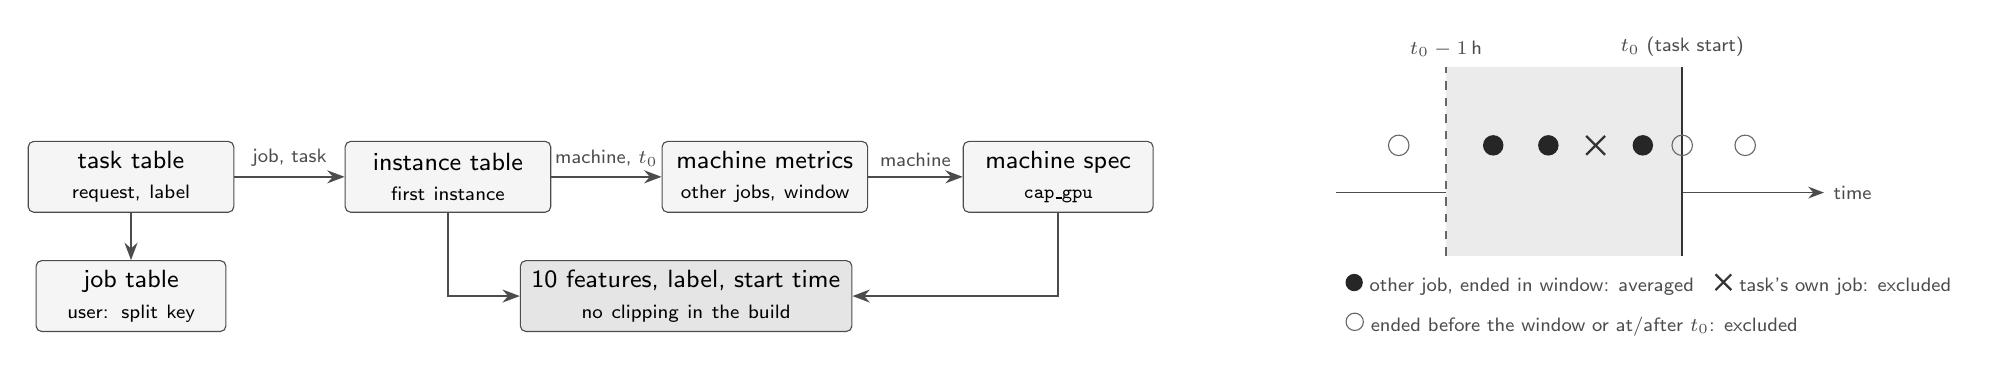
\begin{tikzpicture}[
  font=\sffamily\small,
  box/.style={draw=black!70, rounded corners=2pt, fill=black!4, align=center, minimum height=9mm, inner sep=3pt},
  arr/.style={-{Stealth[length=2.2mm]}, black!70, thick},
  lbl/.style={font=\sffamily\scriptsize, black!70, align=center}]
% ---------------------------------------------------------------- join path
\node[box, text width=24mm] (task) {task table\\{\scriptsize request, label}};
\node[box, text width=24mm, right=14mm of task] (inst) {instance table\\{\scriptsize first instance}};
\node[box, text width=24mm, right=14mm of inst] (mm) {machine metrics\\{\scriptsize other jobs, window}};
\node[box, text width=22mm, right=12mm of mm] (spec) {machine spec\\{\scriptsize \texttt{cap\_gpu}}};
\node[box, text width=22mm, below=6mm of task] (job) {job table\\{\scriptsize user: split key}};
\node[box, text width=40mm, below=6mm of mm, xshift=-10mm, fill=black!10] (feat) {10 features, label, start time\\{\scriptsize no clipping in the build}};
\draw[arr] (task) -- node[lbl, above] {job, task} (inst);
\draw[arr] (inst) -- node[lbl, above] {machine, $t_0$} (mm);
\draw[arr] (mm) -- node[lbl, above] {machine} (spec);
\draw[arr] (task) -- (job);
\draw[arr] (inst.south) |- (feat.west);
\draw[arr] (spec.south) |- (feat.east);
% ---------------------------------------------------------------- the window on a time axis
\begin{scope}[xshift=153mm, yshift=4mm]
  \draw[-{Stealth[length=2mm]}, black!70] (0,-6mm) -- (62mm,-6mm) node[right, lbl] {time};
  \fill[black!8] (14mm,-14mm) rectangle (44mm,10mm);
  \draw[black!60, dashed] (14mm,-14mm) -- (14mm,10mm) node[above, lbl] {$t_0-1\,$h};
  \draw[black!80, thick] (44mm,-14mm) -- (44mm,10mm) node[above, lbl] {$t_0$ (task start)};
  % metric rows plotted at their end time
  \foreach \x/\kind in {8/out, 20/in, 27/in, 33/own, 39/in, 44/edge, 52/out} {
    \ifthenelse{\equal{\kind}{in}}{\fill[black!85] (\x mm,0) circle (1.3mm);}{}
    \ifthenelse{\equal{\kind}{out}}{\draw[black!60] (\x mm,0) circle (1.3mm);}{}
    \ifthenelse{\equal{\kind}{edge}}{\draw[black!60] (\x mm,0) circle (1.3mm);}{}
    \ifthenelse{\equal{\kind}{own}}{\draw[black!80, thick] (\x mm-1.2mm,-1.2mm) -- (\x mm+1.2mm,1.2mm) (\x mm-1.2mm,1.2mm) -- (\x mm+1.2mm,-1.2mm);}{}
  }
  \node[lbl, anchor=north west] at (0mm,-15mm) {\tikz\fill[black!85] (0,0) circle (1.1mm); other job, ended in window: averaged\quad
     \tikz\draw[black!80, thick] (-1mm,-1mm) -- (1mm,1mm) (-1mm,1mm) -- (1mm,-1mm); task's own job: excluded};
  \node[lbl, anchor=north west] at (0mm,-20mm) {\tikz\draw[black!60] (0,0) circle (1.1mm); ended before the window or at/after $t_0$: excluded};
\end{scope}
\end{tikzpicture}}
\caption{Left: the join path from the raw tables to the feature matrix. The user joins only as a split key. Right: the leak-free window. For a task that starts at $t_0$, the five telemetry features average the machine-metric rows of other jobs' workers on the task's machine that ended in $[t_0-1\,\mathrm{h},\, t_0)$; rows of the task's own job and rows ending at or after $t_0$ are never used.}
\label{fig:pipeline}
\end{\pipelinefig}


\subsection{The full trace and the original sample}
The first version of this study built its matrix from a stratified sample of \V{data.v1.sample} labelled tasks and kept the \V{data.orig.tasks} that survived the rules. Here we apply the same rules to every labelled task. Caching the instance table once and computing the windows with vectorised searches makes the build take \V{data.build.minutes} minutes on a laptop with \V{data.ram} of memory. Table~\ref{tab:attrition} and Figure~\ref{fig:attrition} give the attrition: \V{data.full.tasks} tasks survive (\V{data.full.share} of the labelled tasks), with \V{data.full.fail} failures (\V{data.full.rate}) from \V{users.full.users} users. Two steps remove almost all of the lost tasks. At the telemetry step \V{data.tele.nowindow} tasks are lost because no other job's metric row ended on their machine in the window, \V{data.tele.nomachine} because their machine has no telemetry at all, and \V{data.tele.other} because their first instance never started or has no machine. At the last step \V{data.missing.tasks} tasks are lost because a telemetry value is missing. The failure rate rises from \V{data.lab.rate} to \V{data.full.rate} along the way, so the surviving tasks are a selected population. Taking the original \V{data.orig.tasks} tasks from the full build reproduces the first version's matrix value for value before clipping (largest relative difference \V{data.v1.maxrel}), and the same holds for its four other lookback windows. We keep those tasks as the \emph{original sample}, so every protocol can be compared with the first version.

% Generated by scripts/paper_tables.py. Do not edit.
\begin{table}[t]
\centering
\small
\TabCaption{tab:attrition}{Attrition of the full trace at a 1\,h lookback}{Each row is the number of tasks that pass every step up to and including it. A task can lack several features at once, so the counts of missing features overlap.}
\begin{tabular}{@{}lrr@{}}
\toprule
Step & Tasks & Failure rate \\
\midrule
Task table & 1,261,050 &  \\
Labelled (Failed or Terminated) & 1,141,835 & 22.5\% \\
First instance found & 1,141,835 & 22.5\% \\
Telemetry from other jobs in the window & 791,592 & 26.5\% \\
Machine in the specification table & 791,592 & 26.5\% \\
No missing feature & 539,816 & 27.4\% \\
\midrule
\multicolumn{3}{@{}l}{\emph{Lost at the telemetry step}} \\
\quad no other job's row ended in the window & 306,674 & \\
\quad machine has no telemetry at all & 43,537 & \\
\quad first instance never started & 31 & \\
\quad first instance has no machine & 1 & \\
\multicolumn{3}{@{}l}{\emph{Missing at the last step (overlapping)}} \\
\quad \feat{avg_load_1} missing & 103,766 & \\
\quad \feat{avg_cpu_kernel} missing & 102,101 & \\
\quad \feat{avg_cpu_usr} missing & 90,482 & \\
\quad \feat{avg_gpu_util} missing & 87,393 & \\
\quad \feat{avg_net_receive} missing & 76,872 & \\
\quad \feat{plan_gpu} missing & 37,914 & \\
\bottomrule
\end{tabular}
\TabNotes
\end{table}


\begin{figure}[t]
\centering
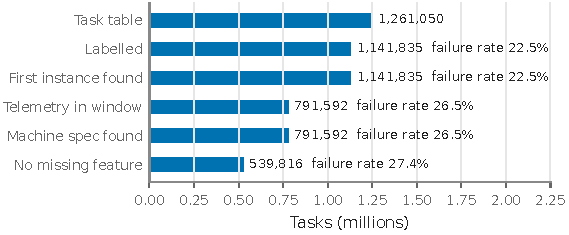
\includegraphics[width=0.62\linewidth]{figures/attrition.pdf}
\caption{Attrition of the full trace at a one-hour lookback: tasks remaining after each step, with the failure rate among them.}
\label{fig:attrition}
\end{figure}

\subsection{Clipping and scaling per split}
The first version clipped every feature at its 1st and 99th percentiles over all rows before splitting, so the clip bounds carried information from the rows that later formed the validation and test sets. In this version the build returns raw values, and each protocol fits the clip bounds and the min-max scaling on its training split alone and applies them unchanged to the validation and test splits. A unit test moves every test row to an extreme value and checks that no fitted constant changes. All models receive identical inputs.

\subsection{Who submits the failures}
Failures are concentrated in a few users (Figure~\ref{fig:concentration}). In the full trace the largest user, User~1, submits \V{users.full.u1.taskshare} of the tasks and \V{users.full.u1.failshare} of the failures, with a failure rate of \V{users.full.u1.rate}. User~4, fourth by task count, submits \V{users.full.u4.taskshare} of the tasks with a failure rate of \V{users.full.u4.rate}. Together the two hold \V{users.full.u14.failshare} of all failures, and the ten users with the most failures hold \V{users.full.top10.failshare}. The original sample has the same structure (User~1: \V{users.orig.u1.taskshare} of the tasks, \V{users.orig.u1.failshare} of the failures). A random task-level split therefore places most of these users' tasks on both sides of the split.

\begin{figure}[t]
\centering
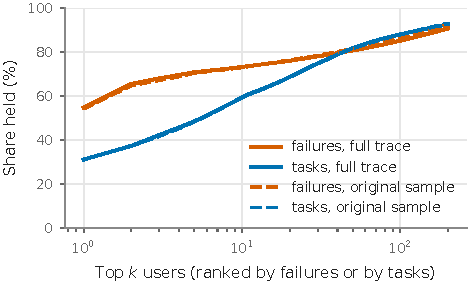
\includegraphics[width=0.62\linewidth]{figures/concentration.pdf}
\caption{Share of all failures (vermillion) and of all tasks (blue) held by the $k$ users with the most failures or the most tasks; full trace solid, original sample dashed. The horizontal axis is logarithmic.}
\label{fig:concentration}
\end{figure}

\section{Model}
\label{sec:model}

\subsection{The Kolmogorov-Arnold additive model}
For a task with scaled features $x_1,\dots,x_d$ ($d=\V{model.d}$), \kaam{} predicts
\begin{equation}
p(\text{fail}\mid x)=\sigma\Big(b+\sum_{i=1}^{d}\phi_i(x_i)\Big),\qquad
\phi_i(x)=w_i\,\mathrm{SiLU}(x)+\sum_{j}c_{ij}B_j(x),
\label{eq:kaam}
\end{equation}
which is the KAN edge form~\cite{liu2025kan} applied once per feature. The $B_j$ are cubic B-splines~\cite{deboor1978splines} on a clamped uniform knot vector with \V{model.knots} interior knots, extended by \V{model.extend} beyond the unit interval on each side; inputs outside the grid are clamped to it. Each feature has \V{model.nbasis} spline coefficients and one SiLU weight, so the model has \V{model.params} parameters. The ten edge functions are stored in a PyTorch \texttt{ModuleDict} keyed by feature name, and the forward pass passes column $i$ to edge $i$ alone, so no edge can read another feature. A unit test perturbs one input and checks that every other contribution is unchanged. The cost of this structure is that \kaam{} cannot represent interactions between features.

\subsection{Training}
The loss is binary cross-entropy plus a smoothness penalty on the spline coefficients,
\begin{equation}
\mathcal{L}=\mathrm{BCE}+\lambda\sum_{i}\sum_{j}\big(c_{i,j+1}-2c_{i,j}+c_{i,j-1}\big)^2,
\end{equation}
which charges curvature and leaves straight segments free, as in P-splines~\cite{eilers1996psplines}. We choose $\lambda$ on the validation split from \V{model.lambdas}. Training uses Adam~\cite{kingma2015adam} with learning rate \V{model.lr} and minibatches of \V{model.batch} tasks. After each epoch the model is scored on the validation split; training stops after \V{model.patience} epochs in which the best validation ROC-AUC has not risen by more than \V{model.mindelta}, and the weights of the best epoch are restored. The cap is \V{model.maxepochs} epochs. The protocol first specified early stopping on validation log loss. We replaced it before any test label was read (Appendix~\ref{app:deviations}): under the time-ordered split the validation failure rate is about three times the training rate, so a barely trained network that predicts about one half everywhere had a lower validation log loss than a trained one, and training stopped after the first epoch. ROC-AUC does not depend on the base rate and is already the selection metric. The first version trained with full batches and a cap of \V{v1.maxepochs} epochs, which every run on its larger sample reached. Here early stopping ended \V{full.train.kaam.allstopped} one of the \V{full.train.kaam.runs} \kaam{} runs on the full trace before the cap, after at most \V{full.train.kaam.maxepochs} epochs.

Because the knots are fixed, each feature's basis values depend only on the input. We evaluate them once per split with the model's own Cox-de~Boor routine, fit the parameters on them and load the result into the standard module, whose forward pass reproduces the training-time output (a unit test checks this).

\subsection{Reading the model}
The contribution $\phi_i(x_i)$ of each feature is available for every prediction. Only the sum of the offsets of the $\phi_i$ and $b$ is identified, so we centre each contribution on its mean over the training tasks. The centred value reads as the amount, in log-odds, by which this feature makes the task riskier than the average training task. For an additive model these centred values are the interventional SHAP values with the training tasks as background~\cite{lundberg2017shap}, which \SecRef{sec:res-interp} confirms numerically.

\subsection{Baselines}
All baselines receive the same per-split clipped and scaled inputs. Logistic regression with an L2 penalty is the linear additive floor, with $C$ chosen from \V{model.lr.ngrid} values between \V{model.lr.cmin} and \V{model.lr.cmax}. The multilayer perceptron (MLP) is the parameter-matched black box: ReLU hidden layers of sizes \V{model.mlp.shapes} with \V{model.mlp.params} parameters, trained with the same loop and early stopping as \kaam{} at a learning rate of \V{model.mlp.lrs}. LightGBM~\cite{ke2017lightgbm} is the strong tabular baseline: learning rate \V{model.lgbm.lr}, at most \V{model.lgbm.rounds} rounds with early stopping on validation ROC-AUC after \V{model.lgbm.es} rounds without improvement, and a grid over the number of leaves (\V{model.lgbm.leaves}) and the minimum leaf size (\V{model.lgbm.minleaf}). The Explainable Boosting Machine (EBM) of InterpretML~\cite{nori2019interpretml} enters twice: as the additive peer of \kaam{}, with \texttt{interactions=0}, and with its default pairwise interaction terms~\cite{lou2013ga2m}. Both EBMs keep the package defaults otherwise and are not tuned; their own early stopping uses an internal holdout of the training split.

Every stochastic model is trained with \V{prot.seeds} initialisation seeds per split, except where compute forced fewer. The EBMs are fitted on every split of the original sample, the EBM with interactions with five seeds on the random splits and one seed under the other protocols. On the full trace an EBM fit with the package defaults takes hours of CPU time, so there only the additive EBM of the canonical split is fitted, for the comparison of shape functions (Appendix~\ref{app:deviations}). Logistic regression is deterministic and is fitted once per split.

\section{Evaluation protocols}
\label{sec:protocols}

The protocols, models, grids, metrics and statistical tests were written into a protocol file before any model was trained on the new datasets and before any test label was read. The file is self-registered, not deposited with a registry: its SHA-256 is stored with every read of test labels. The original sample was analysed in the first version with the same random split seeds, so the results on it are not confirmatory. Four deviations, all made before the first test access and all driven by validation behaviour or compute, are listed with their reasons in Appendix~\ref{app:deviations}. Test labels are returned by a single function that logs every call with the hash of the protocol file; no test label was read until every model of every protocol had been fitted (Appendix~\ref{app:access}). Each protocol is run on the full trace and on the original sample.

\begin{description}
\item[Random.] Stratified \V{prot.frac} splits into training, validation and test sets, with \V{prot.random.nsplits} split seeds. This is the protocol of the first version.
\item[Time-ordered.] Tasks are sorted by the start time of their first instance. The earliest \V{prot.time.train} train, the next \V{prot.time.val} validate and the last \V{prot.time.test} test, which on the full trace covers the last \V{full.split.time.t.testdays} days of the telemetry span. A test task is \emph{known-user} if its user has at least one training task and \emph{new-user} otherwise; we report all test tasks and each subset.
\item[User-grouped.] Five-fold \texttt{StratifiedGroupKFold}~\cite{pedregosa2011sklearn} with the user as the group (seed~0). Within the remaining users of each fold, a second grouped split selects the validation users, so no user appears in two of the three sets. We report the mean and standard deviation over the \V{prot.folds} folds and every fold.
\item[Leave-dominant-user-out.] Users are numbered by task count: User~1 has the most tasks, and User~4, fourth by tasks, is second by failures in the original sample. We remove every task of User~1, and separately of Users~1 and~4, and apply the random split with the canonical seed. This asks how much of the random-split result depends on the two users who hold most failures.
\end{description}

\paragraph{Selection.} For each split, each model's hyperparameters are chosen on the validation split, using the first initialisation seed, by validation ROC-AUC; ties within \V{stat.tie} go to the more regularised setting. The chosen setting is then used for every seed. No choice uses a test split.

\paragraph{Metrics.} ROC-AUC is the primary metric. We also report the area under the precision-recall curve (PR-AUC, computed as average precision), the Brier score~\cite{brier1950verification} and the expected calibration error (ECE) over \V{stat.bins} equal-width bins~\cite{guo2017calibration}, with reliability diagrams on the same bins. No decision threshold is tuned. A model's score on a protocol is the mean over its test sets of the mean over seeds.

\paragraph{Statistics.} Differences between \kaam{} and each other model use a paired bootstrap~\cite{efron1993bootstrap} with \V{stat.nboot} resamples. Tasks are resampled within each test set; for the user-grouped protocol whole users are resampled, since the user is the unit of generalisation there. Every model is scored on the same resamples. We report 95\% percentile intervals and two-sided bootstrap $p$-values, adjusted with Holm's method~\cite{holm1979simple} within each protocol's family of comparisons with \kaam{} (three on the full trace, where the EBMs are absent, and five on the original sample). The intervals resample test tasks with the fitted models held fixed, so they describe uncertainty about the test population and not training or fold variation; for the protocols with several test sets we also report the spread over splits or folds. A difference is \emph{not significant} when the adjusted $p$-value is at least \V{stat.alpha}. \kaam{} \emph{matches} a model when the interval of the difference lies within $\pm$\V{stat.margin} AUC. For the user-grouped protocol we also test each model's fold-mean AUC against chance with the user-level bootstrap, with Holm adjustment over the six models.

\section{Results}
\label{sec:results}

Table~\ref{tab:bench_main} gives the test ROC-AUC of every model under every protocol on both datasets, and Figure~\ref{fig:bench} shows the same numbers with their intervals. Every paired comparison with \kaam{} is listed in Appendix~\ref{app:more}.

% Generated by scripts/paper_tables.py. Do not edit.
\begin{table*}[t]
\centering
\footnotesize
\setlength{\tabcolsep}{3.5pt}
\TabCaption{tab:bench_main}{Test ROC-AUC of every model under every protocol}{Mean over test sets (five splits or folds where applicable) of the mean over seeds, with the 95\% bootstrap interval below (tasks resampled; users for the user-grouped protocol). Bold: best model in the column of each panel. $^{\circ}$: the difference from \kaam{} is not significant after Holm correction. Intervals resample test tasks with the fitted models held fixed, so they do not include training or fold variation. Under the protocols the EBMs were fitted on the original sample only (compute; Appendix~\ref{app:deviations}).}
\begin{tabular}{@{}lccccccc@{}}
\toprule
Model & \begin{tabular}[b]{@{}c@{}}Random\end{tabular} & \begin{tabular}[b]{@{}c@{}}Time,\\all users\end{tabular} & \begin{tabular}[b]{@{}c@{}}Time,\\known users\end{tabular} & \begin{tabular}[b]{@{}c@{}}Time,\\new users\end{tabular} & \begin{tabular}[b]{@{}c@{}}User-\\grouped\end{tabular} & \begin{tabular}[b]{@{}c@{}}Without\\User~1\end{tabular} & \begin{tabular}[b]{@{}c@{}}Without\\Users~1,~4\end{tabular} \\
\midrule
\multicolumn{8}{@{}l}{\emph{Full trace (\V{data.full.tasks} tasks)}} \\
KAAM & 0.766 & 0.594 & 0.596 & 0.466 & \textbf{0.641} & 0.703 & 0.672 \\
 & {\tiny [0.764, 0.767]} & {\tiny [0.589, 0.599]} & {\tiny [0.591, 0.601]} & {\tiny [0.424, 0.508]} & {\tiny [0.527, 0.670]} & {\tiny [0.698, 0.709]} & {\tiny [0.665, 0.678]} \\[1pt]
Logistic regression & 0.732 & 0.576 & 0.580 & 0.462$^{\circ}$ & 0.600 & 0.656 & 0.630 \\
 & {\tiny [0.730, 0.734]} & {\tiny [0.571, 0.581]} & {\tiny [0.574, 0.585]} & {\tiny [0.420, 0.504]} & {\tiny [0.491, 0.633]} & {\tiny [0.650, 0.662]} & {\tiny [0.623, 0.637]} \\[1pt]
MLP & 0.804 & 0.596$^{\circ}$ & \textbf{0.599}$^{\circ}$ & 0.482$^{\circ}$ & 0.637$^{\circ}$ & 0.721 & 0.698 \\
 & {\tiny [0.802, 0.805]} & {\tiny [0.592, 0.601]} & {\tiny [0.594, 0.604]} & {\tiny [0.445, 0.521]} & {\tiny [0.539, 0.664]} & {\tiny [0.716, 0.726]} & {\tiny [0.692, 0.704]} \\[1pt]
LightGBM & \textbf{0.900} & \textbf{0.599}$^{\circ}$ & \textbf{0.599}$^{\circ}$ & \textbf{0.534} & 0.566$^{\circ}$ & \textbf{0.845} & \textbf{0.805} \\
 & {\tiny [0.899, 0.901]} & {\tiny [0.594, 0.604]} & {\tiny [0.594, 0.604]} & {\tiny [0.496, 0.573]} & {\tiny [0.520, 0.599]} & {\tiny [0.841, 0.849]} & {\tiny [0.799, 0.810]} \\[1pt]
\midrule
\multicolumn{8}{@{}l}{\emph{Original sample (\V{data.orig.tasks} tasks)}} \\
KAAM & 0.744 & 0.595 & 0.603 & 0.515 & \textbf{0.620} & 0.698 & 0.627 \\
 & {\tiny [0.735, 0.754]} & {\tiny [0.572, 0.618]} & {\tiny [0.579, 0.629]} & {\tiny [0.423, 0.605]} & {\tiny [0.551, 0.641]} & {\tiny [0.667, 0.728]} & {\tiny [0.591, 0.665]} \\[1pt]
Logistic regression & 0.723 & 0.588$^{\circ}$ & 0.589$^{\circ}$ & \textbf{0.565}$^{\circ}$ & 0.561$^{\circ}$ & 0.662 & 0.602 \\
 & {\tiny [0.713, 0.732]} & {\tiny [0.561, 0.614]} & {\tiny [0.561, 0.618]} & {\tiny [0.458, 0.666]} & {\tiny [0.487, 0.601]} & {\tiny [0.632, 0.693]} & {\tiny [0.563, 0.640]} \\[1pt]
MLP & 0.722 & 0.523 & 0.533 & 0.548$^{\circ}$ & 0.540 & 0.681$^{\circ}$ & 0.531 \\
 & {\tiny [0.714, 0.729]} & {\tiny [0.499, 0.547]} & {\tiny [0.507, 0.558]} & {\tiny [0.462, 0.628]} & {\tiny [0.486, 0.564]} & {\tiny [0.652, 0.709]} & {\tiny [0.516, 0.544]} \\[1pt]
LightGBM & \textbf{0.810} & \textbf{0.619}$^{\circ}$ & \textbf{0.620}$^{\circ}$ & 0.552$^{\circ}$ & 0.502$^{\circ}$ & \textbf{0.756} & 0.673 \\
 & {\tiny [0.801, 0.818]} & {\tiny [0.595, 0.642]} & {\tiny [0.595, 0.647]} & {\tiny [0.461, 0.640]} & {\tiny [0.469, 0.577]} & {\tiny [0.728, 0.784]} & {\tiny [0.642, 0.706]} \\[1pt]
EBM, additive & 0.756 & 0.595$^{\circ}$ & 0.596$^{\circ}$ & 0.533$^{\circ}$ & 0.489$^{\circ}$ & 0.722 & 0.646 \\
 & {\tiny [0.746, 0.765]} & {\tiny [0.571, 0.620]} & {\tiny [0.572, 0.621]} & {\tiny [0.423, 0.636]} & {\tiny [0.454, 0.588]} & {\tiny [0.693, 0.752]} & {\tiny [0.611, 0.682]} \\[1pt]
EBM, pairwise & 0.803 & 0.573$^{\circ}$ & 0.565$^{\circ}$ & 0.539$^{\circ}$ & 0.504$^{\circ}$ & 0.752 & \textbf{0.685} \\
 & {\tiny [0.794, 0.811]} & {\tiny [0.545, 0.601]} & {\tiny [0.535, 0.596]} & {\tiny [0.430, 0.641]} & {\tiny [0.466, 0.599]} & {\tiny [0.724, 0.781]} & {\tiny [0.650, 0.720]} \\[1pt]
\bottomrule
\end{tabular}
\TabNotes
\end{table*}


\begin{figure*}[t]
\centering
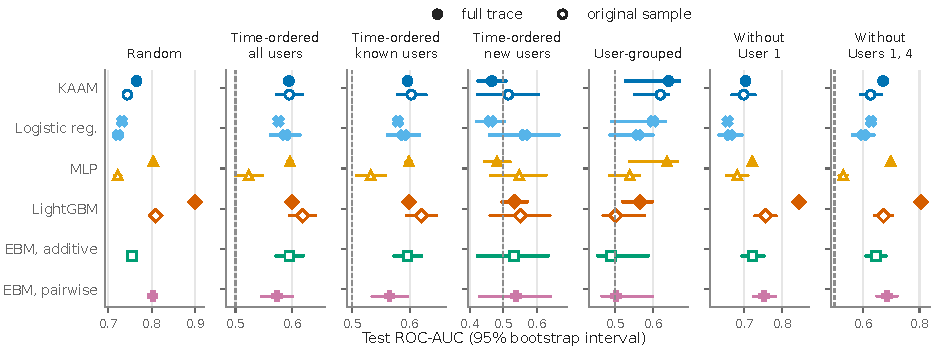
\includegraphics[width=\textwidth]{figures/benchmark.pdf}
\caption{Test ROC-AUC with 95\% bootstrap intervals for every model and protocol; filled markers: full trace, open markers: original sample. The EBMs were fitted on the original sample only. Dashed line: chance. Each panel has its own horizontal scale.}
\label{fig:bench}
\end{figure*}

\subsection{Random splits}
\label{sec:res-random}

On the full trace \kaam{} reaches \V{full.random.kaam.auc} \V{full.random.kaam.ci}. It is above logistic regression by \V{full.random.lr.diff} (\V{full.random.lr.dci}, \V{full.random.lr.sig}) and below the parameter-matched MLP by \V{full.random.mlp.absdiff} (\V{full.random.mlp.dci}) and LightGBM by \V{full.random.lgbm.absdiff} (\V{full.random.lgbm.dci}); both differences are \V{full.random.lgbm.sig}. On the original sample, where all six models were fitted, \kaam{} reaches \V{orig.random.kaam.auc}: above logistic regression (\V{orig.random.lr.diff}) and the MLP (\V{orig.random.mlp.diff}), slightly below the additive EBM (\V{orig.random.ebm.diff}, \V{orig.random.ebm.dci}), and well below the two models with interactions, LightGBM (\V{orig.random.lgbm.diff}) and the EBM with pairwise terms (\V{orig.random.ebmi.diff}). All five differences are \V{orig.random.lgbm.sig} after Holm correction, and none lies within the $\pm$\V{stat.margin} margin, so \kaam{} matches none of the baselines. The two additive models are close to each other and the two models with interactions are close to each other, with a gap of about \V{orig.random.ebmi.absdiff} between the pairs. The MLP is weaker on the original sample than in the first version (\V{orig.random.mlp.auc} over five splits, against \V{v1.mlp.auc} on one split there); the first version's best learning rate is not in the present grid, and the networks now stop on validation AUC. The spread between splits is small next to these gaps (\kaam{}: standard deviation \V{orig.random.kaam.setstd} over the five splits of the original sample and \V{full.random.kaam.setstd} on the full trace).

\paragraph{Exact duplicates.} In each random split of the full trace, \V{rf.full.dup.random.min} to \V{rf.full.dup.random.max} of the test tasks have an exact copy of all ten raw features among the training tasks: concurrent submissions of the same request that land on the same machine within the same window. Under the time-ordered split the share is \V{rf.full.dup.time.max}, in the user-grouped folds \V{rf.full.dup.grouped.min} to \V{rf.full.dup.grouped.max}, and in the original sample, which samples the trace sparsely, \V{rf.orig.dup.random.min} to \V{rf.orig.dup.random.max}. A random split of the full trace therefore rewards recognising duplicated requests as well as known users. The larger random-split score of LightGBM on the full trace than on the original sample (\V{full.random.lgbm.auc} against \V{orig.random.lgbm.auc}) is consistent with this, although we did not separate the two effects. This check was added after an independent review.

\paragraph{Calibration.} PR-AUC and the Brier score order the models as ROC-AUC does (Table~\ref{tab:calib_full}). Under the random protocol LightGBM, the MLP and \kaam{} are close to calibrated on the full trace (ECE \V{full.random.lgbm.ece}, \V{full.random.mlp.ece} and \V{full.random.kaam.ece}), and logistic regression is less so (\V{full.random.lr.ece}; Figure~\ref{fig:reliability}). Under the time-ordered and user-grouped protocols the base rate of the test tasks differs from that of the training tasks, and calibration degrades (ECE \V{full.time.minece} to \V{full.time.maxece} and \V{full.grouped.minece} to \V{full.grouped.maxece}).

% Generated by scripts/paper_tables.py. Do not edit.
\begin{table}[t]
\centering
\small
\setlength{\tabcolsep}{3pt}
\TabCaption{tab:calib_full}{Precision-recall and calibration, full trace}{PR-AUC is average precision; Brier score and expected calibration error (ECE, 15 equal-width bins) are lower-is-better. Means over test sets and seeds.}
\begin{tabular}{@{}lccccccccc@{}}
\toprule
 & \multicolumn{3}{c}{Random} & \multicolumn{3}{c}{Time, all} & \multicolumn{3}{c}{User-grouped} \\
\cmidrule(lr){2-4}\cmidrule(lr){5-7}\cmidrule(lr){8-10}
Model & PR-AUC & Brier & ECE & PR-AUC & Brier & ECE & PR-AUC & Brier & ECE \\
\midrule
KAAM & 0.641 & 0.149 & 0.034 & 0.211 & 0.142 & 0.069 & 0.355 & 0.172 & 0.112 \\
Logistic regression & 0.546 & 0.165 & 0.084 & 0.191 & 0.141 & 0.066 & 0.336 & 0.182 & 0.133 \\
MLP & 0.685 & 0.136 & 0.018 & 0.211 & 0.139 & 0.056 & 0.370 & 0.173 & 0.105 \\
LightGBM & 0.849 & 0.093 & 0.017 & 0.196 & 0.139 & 0.051 & 0.304 & 0.183 & 0.105 \\
\bottomrule
\end{tabular}
\TabNotes
\end{table}


\begin{figure*}[t]
\centering
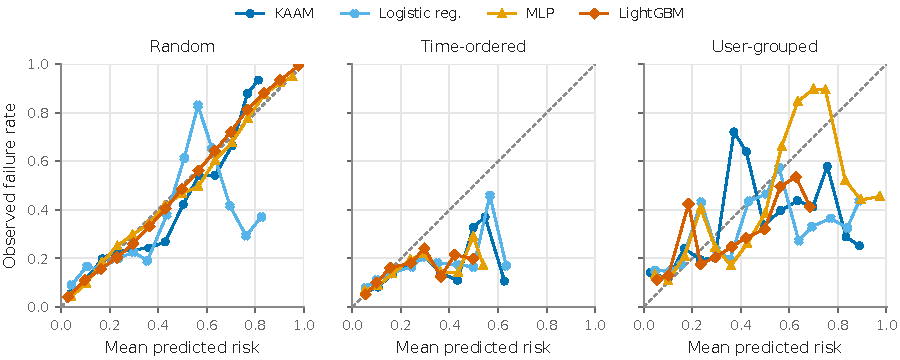
\includegraphics[width=\textwidth]{figures/reliability.pdf}
\caption{Reliability diagrams on the full trace (first seed, test sets of a protocol pooled, bins with at least \V{fig.minbin} tasks). Dashed: perfect calibration.}
\label{fig:reliability}
\end{figure*}

\subsection{Time-ordered split}
\label{sec:res-time}

Training on the first \V{prot.time.train} of the full trace by start time and testing on the last \V{prot.time.test}, which spans \V{full.split.time.t.testdays} days, every model drops to between \V{full.time.minauc} and \V{full.time.maxauc}. \kaam{} reaches \V{full.time.kaam.auc} \V{full.time.kaam.ci} and LightGBM \V{full.time.lgbm.auc} \V{full.time.lgbm.ci}; their difference is \V{full.time.lgbm.sig}. The drop is not an effect of new users: \V{full.split.time.t.knownshare} of the test tasks come from users with training tasks, and on those tasks the models score between \V{full.timeknown.minauc} and \V{full.timeknown.maxauc}. The \V{full.split.time.t.newn} test tasks of new users are scored between \V{full.timenew.minauc} and \V{full.timenew.maxauc} (\kaam{}: \V{full.timenew.kaam.auc} \V{full.timenew.kaam.ci}). The period matters more than the user here. The validation period, the \V{prot.time.val} of tasks just before the test period, is a burst dominated by User~1, who submits \V{rf.full.time.val.u1} of its tasks against \V{rf.full.time.train.u1} of the training tasks and \V{rf.full.time.test.u1} of the test tasks. Its failure rate is \V{full.split.time.t.rateval} (\V{rf.full.time.val.rateno1} without User~1), against \V{full.split.time.t.ratetrain} in training and \V{full.split.time.t.ratetest} in test, and on it the same models reached validation AUCs between \V{full.time.minvalauc} and \V{full.time.maxvalauc}; the networks stopped after about \V{full.time.mlp.bestepoch} epochs (MLP) and \V{full.time.kaam.bestepoch} (\kaam{}). Model selection on this period overstated the accuracy in the test week, which starts \V{rf.full.time.gap} days after the last training task. The \V{full.split.time.t.newn} new-user test tasks come from \V{rf.full.time.newusers} users; on them LightGBM is the best model, above \kaam{} by \V{full.timenew.lgbm.absdiff} (\V{full.timenew.lgbm.sig} under the task-level bootstrap, which treats these tasks as independent although they come from few users). The original sample shows the same pattern (Table~\ref{tab:bench_main}).

\subsection{User-grouped folds}
\label{sec:res-grouped}

With users held out, the full-trace AUCs fall to between \V{full.grouped.minauc} and \V{full.grouped.maxauc} (Table~\ref{tab:grouped_full}, Figure~\ref{fig:folds}). The five folds are unequal. StratifiedGroupKFold places User~1 with two small users in fold~\V{full.mech.u1fold}, whose \V{full.mech.u1.ntest} test tasks come from \V{full.mech.u1.testusers} users, so that fold is in effect a test on User~1 alone and its user-level interval rests on three clusters; the other folds hold \V{full.mech.nou.min.users} to \V{full.mech.nou.max.users} test users each. On those \V{full.gnou.nfolds} folds the mean AUCs are \V{full.gnou.mlp.auc} for the MLP, \V{full.gnou.kaam.auc} for \kaam{}, \V{full.gnou.lr.auc} for logistic regression and \V{full.gnou.lgbm.auc} for LightGBM; on the fold with User~1 they are \V{full.gu1.kaam.auc}, \V{full.gu1.mlp.auc}, \V{full.gu1.lr.auc} and \V{full.gu1.lgbm.auc} for \kaam{}, the MLP, logistic regression and LightGBM. Over all five folds \kaam{} has the highest mean, \V{full.grouped.kaam.auc} \V{full.grouped.kaam.ci}, but its differences from the MLP (\V{full.grouped.mlp.diff}, \V{full.grouped.mlp.dci}) and from LightGBM (\V{full.grouped.lgbm.diff}, \V{full.grouped.lgbm.dci}) are not significant, the interval of the difference with the MLP extends past the $\pm$\V{stat.margin} margin on both sides, and the ranking depends on how the folds are combined. No model is clearly best on new users. LightGBM's grouped fits stopped early: their mean best iteration ranges from \V{full.lgbm.grouped.minrounds} to \V{full.lgbm.grouped.maxrounds} boosting rounds over the folds, against \V{full.lgbm.random.minrounds} to \V{full.lgbm.random.maxrounds} on the random splits, and its seed-to-seed spread is \V{full.grouped.lgbm.seedstd} against \V{full.grouped.kaam.seedstd} for \kaam{}. Its low grouped score reflects ensembles that early stopping on validation users cut almost at once; a more strongly regularised or interaction-constrained boosting model was not tested. On the original sample \kaam{} leads on the \V{orig.gnou.nfolds} folds without User~1 (\V{orig.gnou.kaam.auc} against \V{orig.gnou.min} to \V{orig.gnou.lr.auc} for the other models), on about three thousand test tasks per fold. Against chance, \V{full.chance.nsig} of the \V{full.chance.nmodels} full-trace models and \V{orig.chance.nsig} of the \V{orig.chance.nmodels} original-sample models are significantly above 0.5 after Holm correction, and none is significantly below it. Fold AUCs on the full trace range from \V{full.fold.minauc} to \V{full.fold.maxauc}, and \V{full.fold.nbelow} of the \V{full.fold.npairs} fold-model pairs fall below 0.5.

% Generated by scripts/paper_tables.py. Do not edit.
\begin{table*}[t]
\centering
\footnotesize
\setlength{\tabcolsep}{3pt}
\TabCaption{tab:grouped_full}{User-grouped folds on the full trace}{AUC per fold (mean over seeds), the fold mean with a user-level bootstrap interval and its Holm-adjusted $p$-value against 0.5, and the one-core mechanism per fold.}
\begin{tabular}{@{}lcccccccc@{}}
\toprule
Model & Fold 0 & Fold 1 & Fold 2 & Fold 3 & Fold 4 & Mean & 95\% CI & $p_{\mathrm{Holm}}$ vs.\ 0.5 \\
\midrule
KAAM & 0.581 & 0.551 & 0.559 & 0.760 & 0.754 & 0.641 & [0.527, 0.670] & 0.014 \\
Logistic regression & 0.586 & 0.496 & 0.486 & 0.782 & 0.651 & 0.600 & [0.491, 0.633] & 0.095 \\
MLP & 0.563 & 0.540 & 0.595 & 0.799 & 0.686 & 0.637 & [0.539, 0.664] & 0.004 \\
LightGBM & 0.522 & 0.574 & 0.626 & 0.490 & 0.616 & 0.566 & [0.520, 0.599] & 0.006 \\
\midrule
Test users & 288 & 278 & 277 & 313 & 3 &  &  &  \\
Test tasks & 86,778 & 86,746 & 86,800 & 86,745 & 192,747 &  &  &  \\
One-core failure rate, train & 82.5\% & 77.1\% & 82.6\% & 78.2\% & 19.5\% &  &  &  \\
Other failure rate, train & 20.4\% & 20.5\% & 20.6\% & 19.0\% & 19.5\% &  &  &  \\
One-core failure rate, test & 27.8\% & 36.5\% & 15.0\% & 16.3\% & 87.2\% &  &  &  \\
Other failure rate, test & 17.4\% & 17.3\% & 18.1\% & 23.1\% & 20.6\% &  &  &  \\
AUC of $-$\feat{plan_cpu}, train & 0.734 & 0.728 & 0.727 & 0.694 & 0.559 &  &  &  \\
AUC of $-$\feat{plan_cpu}, test & 0.455 & 0.474 & 0.431 & 0.717 & 0.765 &  &  &  \\
\bottomrule
\end{tabular}
\TabNotes
\end{table*}


\begin{figure}[t]
\centering
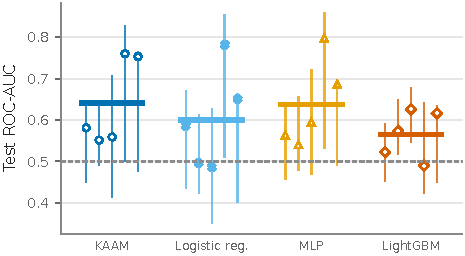
\includegraphics[width=0.62\linewidth]{figures/grouped_folds.pdf}
\caption{User-grouped folds on the full trace. Open markers: AUC of each fold (mean over seeds) with its user-level 95\% interval; bar: mean over folds. Dashed line: chance.}
\label{fig:folds}
\end{figure}

\paragraph{Why some folds fall below chance.} In every training split that contains User~1, one-core tasks fail at \V{rf.oc.with.minone} to \V{rf.oc.with.maxone} against \V{rf.oc.with.minother} to \V{rf.oc.with.maxother} for other tasks, and User~1 holds \V{rf.oc.with.minu1} to \V{rf.oc.with.maxu1} of the one-core training tasks. Without User~1 the difference almost disappears: one-core tasks fail at \V{rf.oc.groupedf4.one} against \V{rf.oc.groupedf4.other} among the training users of fold~\V{full.mech.u1fold}, and at \V{rf.oc.louod1.one} against \V{rf.oc.louod1.other} in the split without User~1. Among the held-out users of the other folds the picture is mixed (Table~\ref{tab:grouped_full}, lower rows): one-core tasks fail more often than other tasks in folds~0 and~1 (\V{full.mech.f0.teonerate} and \V{full.mech.f1.teonerate} against \V{full.mech.f0.teotherrate} and \V{full.mech.f1.teotherrate}) and less often in folds~2 and~3 (\V{full.mech.f2.teonerate} and \V{full.mech.f3.teonerate} against \V{full.mech.f2.teotherrate} and \V{full.mech.f3.teotherrate}). Ranking all test tasks by $-$\feat{plan_cpu}, the direction the models learn, gives AUCs of \V{full.mech.nou.min.teauc} to \V{full.mech.nou.max.teauc} on the held-out users, below chance in \V{full.mech.nou.nrev} of these folds: a rule learned largely from User~1 overstates the one-core risk of most other users and orders their larger requests poorly.

\subsection{Leaving out the dominant users}
\label{sec:res-louo}

Removing every task of User~1 changes the test population as well as the training data: User~1's tasks fail at \V{users.full.u1.rate} against \V{users.full.nonu1.rate} for the other users, and their presence makes ranking easier. The AUCs of this protocol are therefore not directly comparable with those of the random protocol, and the protocol does not separate the effect of User~1 on training from its effect on the test set. Without User~1, and without Users~1 and~4, LightGBM still leads \kaam{} by \V{full.louoa.lgbm.absdiff} and \V{full.louob.lgbm.absdiff} (both \V{full.louob.lgbm.sig}). Its random-split lead is therefore not explained by the two dominant users; the exact duplicates described above, \V{rf.full.dup.louo.min} to \V{rf.full.dup.louo.max} of the test tasks of these splits, are one candidate.

\subsection{Interpretability}
\label{sec:res-interp}

\paragraph{The contributions are exact SHAP values.} Kernel SHAP with every one of the \V{shap.coalitions} feature coalitions, a background of \V{shap.background} training tasks and \V{shap.tasks} test tasks returns the centred \kaam{} contributions of the canonical model to within \V{shap.maxdiff} log-odds, and the ten contributions plus the bias reproduce the model's logit to within \V{shap.sumgap}. No sampling enters a \kaam{} explanation; the same holds for any additive model, the additive EBM included, so this property does not favour the KAN parameterisation over other additive models.

\paragraph{The curves.} Figure~\ref{fig:curves} shows the ten curves of the canonical model for its five seeds, with the corresponding curve of the original sample. The five seeds give nearly identical curves. Validation chose no smoothness penalty on all five random splits of the full trace, and the strongest value, \V{model.lambdamax}, on the time-ordered split and on \V{full.lambda.grouped.em2} of the five user-grouped folds, where the validation tasks come from a later period or from other users. On the random splits the four request features therefore get curves that oscillate between the few values that occur (the ticks in Figure~\ref{fig:curves}); such a curve is informative only at observed values. The telemetry curves are smooth: risk rises with the recent kernel CPU of the machine and falls steeply as its recent load rises from low values, the pattern the first version reported and attributed, tentatively, to the trace recording telemetry mostly for workers that finished.

\begin{figure*}[t]
\centering
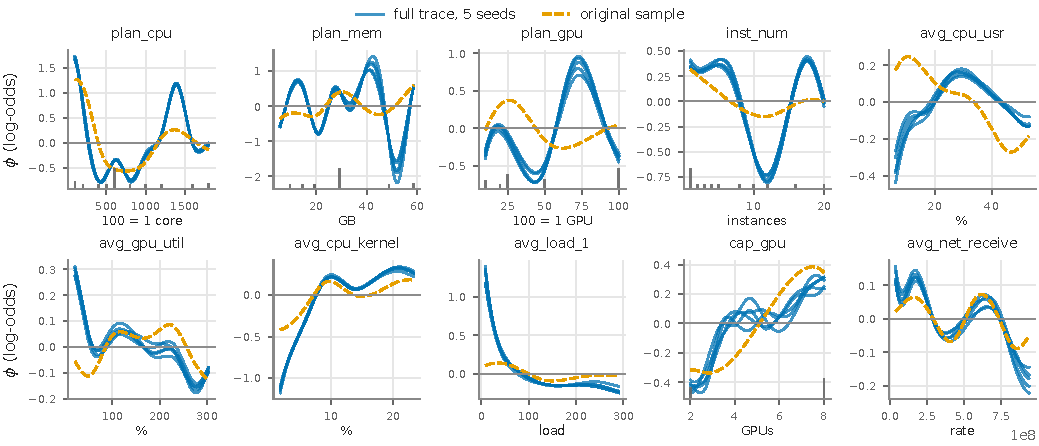
\includegraphics[width=\textwidth]{figures/curves_all.pdf}
\caption{The ten curves of the canonical \kaam{} (full trace, random split \V{prot.canon}) for five seeds, and the curve learned on the original sample (dashed), each centred on its mean over the training 5th to 95th percentile. Ticks: values of the discrete features held by at least \V{fig.tickshare} of training tasks, with height proportional to their share.}
\label{fig:curves}
\end{figure*}

\paragraph{\kaam{} against the additive EBM.} The two additive models fit their shape functions in different ways, B-splines by gradient descent and piecewise-constant terms by cyclic boosting, so their agreement is a check on both (Table~\ref{tab:shapecorr}, Figure~\ref{fig:shapes}). On the grid fixed in the protocol the median correlation over the ten features is \V{ebm.r.median}; the telemetry curves agree closely, while two request features show almost no agreement (lowest: \V{ebm.r.worstfeat}, $r=\V{ebm.r.min}$). Evaluated at the training tasks' own values, an exploratory measure not fixed in the protocol, the median correlation is \V{ebm.rd.median} and the lowest \V{ebm.rd.min} (\V{ebm.rd.worstfeat}). The disagreement is therefore concentrated between observed values of the discrete requests, where neither model has data. On the canonical split the additive EBM, fitted once on the full trace, reaches a test AUC of \V{full.s42.ebm.auc} against \V{full.s42.kaam.auc} for \kaam{}.

% Generated by scripts/paper_tables.py. Do not edit.
\begin{table}[t]
\centering
\small
\TabCaption{tab:shapecorr}{\kaam{} and additive EBM shape functions}{$r_{\mathrm{grid}}$: Pearson correlation of the two centred curves on 200 evenly spaced points between the training 5th and 95th percentiles, as fixed in the protocol. $r_{\mathrm{data}}$ (exploratory): the same correlation at the values of up to \V{ebm.rd.ntasks} training tasks inside that window, so that each value counts as often as it occurs; for the request features, which take few distinct values, the grid version mostly compares how the two models fill the gaps between observed values. Swing: maximum minus minimum of each curve over the window, in log-odds. Canonical random split of the \V{ebm.shapeds}, seed~0.}
\begin{tabular}{@{}lcccc@{}}
\toprule
Feature & $r_{\mathrm{grid}}$ & $r_{\mathrm{data}}$ & \kaam{} swing & EBM swing \\
\midrule
\feat{plan_mem} & 0.04 & 0.75 & 3.16 & 2.97 \\
\feat{plan_cpu} & 0.62 & 0.99 & 2.50 & 2.62 \\
\feat{plan_gpu} & 0.04 & 0.57 & 1.66 & 0.97 \\
\feat{avg_load_1} & 0.97 & 0.97 & 1.61 & 1.79 \\
\feat{avg_cpu_kernel} & 0.98 & 0.99 & 1.47 & 1.71 \\
\feat{inst_num} & 0.46 & 0.81 & 1.22 & 1.17 \\
\feat{cap_gpu} & 0.70 & 1.00 & 0.76 & 0.68 \\
\feat{avg_cpu_usr} & 0.90 & 0.88 & 0.54 & 0.64 \\
\feat{avg_gpu_util} & 0.85 & 0.82 & 0.43 & 0.45 \\
\feat{avg_net_receive} & 0.80 & 0.76 & 0.29 & 0.47 \\
\bottomrule
\end{tabular}
\TabNotes
\end{table}


\begin{figure*}[t]
\centering
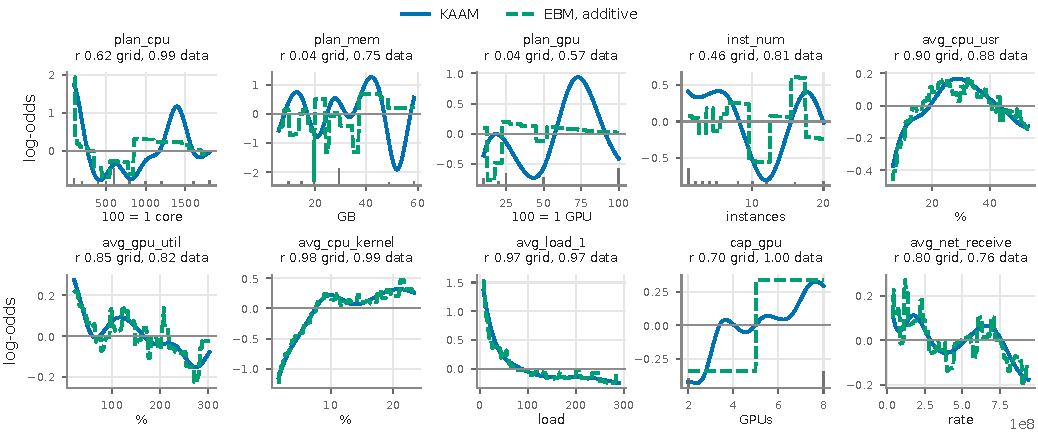
\includegraphics[width=\textwidth]{figures/shapes_kaam_ebm.pdf}
\caption{Shape functions of \kaam{} and of the additive EBM on the canonical split, centred on their means over the training 5th to 95th percentile. Panel titles give the correlation on the protocol's evenly spaced grid and at the training tasks' values. Ticks as in Figure~\ref{fig:curves}.}
\label{fig:shapes}
\end{figure*}

\paragraph{The one-core curve under each protocol.} Figure~\ref{fig:plancpu} overlays the \feat{plan_cpu} curve of the first seed under every protocol of the full trace. On the canonical split the centred curve stands at \V{pc.randoms42.onecore} log-odds at one core. With User~1 removed it stands at \V{pc.louod1.onecore}, and with Users~1 and~4 removed at \V{pc.louod14.onecore}. In the user-grouped folds the value at one core ranges from \V{pc.grouped.minone} to \V{pc.grouped.maxone}; the lowest is fold~\V{full.mech.u1fold}, whose training set also lacks User~1. A centred value reflects the whole shape of a curve as well as the one-core effect, and the shape changes from fit to fit (correlation with the canonical curve between \V{pc.groupedf1.corr} and \V{pc.groupedf0.corr} over the grouped folds, \V{pc.timet.corr} for the time-ordered split), so the training data give the clearer evidence: with User~1 in training, one-core tasks fail at \V{rf.oc.with.minone} to \V{rf.oc.with.maxone} against \V{rf.oc.with.minother} to \V{rf.oc.with.maxother} for other tasks, and without User~1 at \V{rf.oc.groupedf4.one} against \V{rf.oc.groupedf4.other} (fold~\V{full.mech.u1fold}) and \V{rf.oc.louod1.one} against \V{rf.oc.louod1.other} (split without User~1). Centring on the mean training task instead of the grid, a post hoc check, a one-core request adds \V{ph.oc.randoms42} log-odds on the canonical split and \V{ph.oc.gwith.min} to \V{ph.oc.gwith.max} in the grouped folds whose training users include User~1, against \V{ph.oc.louod1} without User~1 and \V{ph.oc.louod14} without Users~1 and~4. Fold~\V{full.mech.u1fold}, trained without User~1, still gives \V{ph.oc.gwithout}, although its one-core and other training tasks fail at \V{ph.oc.gwithout.trone} and \V{ph.oc.gwithout.trother}. The curves are a complete account of each fitted model; they are not a stable account of the data. A second rise near thirteen cores appears with and without User~1 but not in the time-ordered curve.

\begin{figure}[t]
\centering
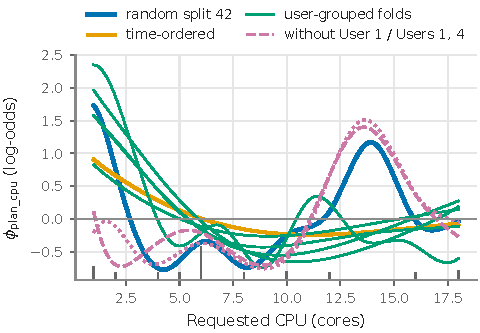
\includegraphics[width=0.62\linewidth]{figures/plan_cpu_protocols.pdf}
\caption{The \feat{plan_cpu} curve of \kaam{} (first seed) under each protocol of the full trace, centred on the same window. Ticks: request values held by at least \V{fig.tickshare} of the canonical training tasks.}
\label{fig:plancpu}
\end{figure}

\subsection{Case audits}
\label{sec:res-cases}

The four cases were selected on the canonical model's test set by the rule fixed in the first version: the most confident true positive and true negative, and the false negative and false positive with the highest risk at a threshold of 0.5 (Table~\ref{tab:cases}, Figure~\ref{fig:waterfall}). Each bar is the contribution of one feature relative to the mean training task, whose logit is \V{case.baselogit}; in every case the ten contributions and the bias reproduce the logit to within \V{case.maxsumgap}.

The true positive (risk \V{case.tp.risk}) is a one-core request, and \feat{plan_cpu} contributes \V{case.tp.c.plancpu}, \V{case.tp.topshare} of the total absolute push. The identical four-field request occurs in \V{case.tp.samereq} training tasks, \V{case.tp.samerate} of which failed and \V{case.tp.sameu1} of which came from User~1. The false positive (risk \V{case.fp.risk}) is also a one-core request and receives the same \V{case.fp.c.plancpu} from \feat{plan_cpu}, plus \V{case.fp.c.planmem} from a large memory request. Its own request occurs in only \V{case.fp.samereq} training tasks, \V{case.fp.samerate} of which failed and none from User~1: the one-core term learned largely from one user's recurring job is applied to another user's task. The false negative (risk \V{case.fn.risk}, just below the threshold) requests half a core (\V{case.fn.c.plancpu}) and \V{case.fn.raw.instnum} instances (\V{case.fn.c.instnum}); its request occurs in \V{case.fn.samereq} training tasks with a failure rate of \V{case.fn.samerate}. The true negative (risk \V{case.tn.risk}) owes most of its score to \feat{plan_gpu} at the \V{case.tn.pct.plangpu} percentile (\V{case.tn.c.plangpu}); its exact request occurs in \V{case.tn.samereq} training tasks, none of which failed. A confident score that rests on a sparse region of one feature is visible at a glance in this form.

% Generated by scripts/paper_tables.py. Do not edit.
\begin{table*}[t]
\centering
\small
\TabCaption{tab:cases}{Four case audits of the canonical \kaam{}}{Selected by the rule fixed in advance (most confident true positive and true negative; highest-risk false negative and false positive at threshold 0.5). Contributions are log-odds relative to the mean training task. Same request: training tasks with the identical four resource requests / their failure rate / the share submitted by User~1.}
\begin{tabular}{@{}lcp{7.2cm}l@{}}
\toprule
Case & Risk & Largest three contributions & Same request \\
\midrule
True positive & 0.861 & \feat{plan_cpu} +1.68; \feat{avg_load_1} +0.41; \feat{avg_cpu_kernel} +0.36 & 44,191 / 87\% / 100\% \\
True negative & 0.002 & \feat{plan_gpu} $-$4.32; \feat{plan_cpu} $-$0.80; \feat{cap_gpu} $-$0.50 & 18 / 0\% / 0\% \\
False negative & 0.500 & \feat{plan_cpu} +1.60; \feat{inst_num} $-$0.86; \feat{cap_gpu} +0.22 & 1,995 / 5\% / 0\% \\
False positive & 0.878 & \feat{plan_cpu} +1.68; \feat{plan_mem} +0.79; \feat{avg_cpu_kernel} +0.26 & 44 / 5\% / 0\% \\
\bottomrule
\end{tabular}
\TabNotes
\end{table*}


\begin{figure*}[t]
\centering
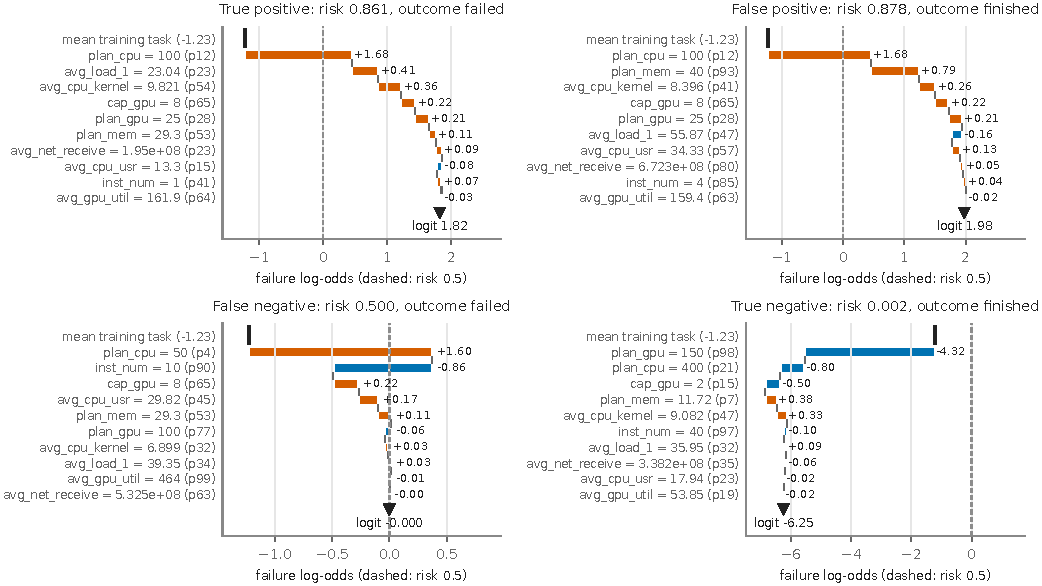
\includegraphics[width=\textwidth]{figures/case_waterfall.pdf}
\caption{Case audits of the canonical \kaam{}. Each panel runs from the logit of the mean training task (top) through the ten contributions, largest first, to the model's logit (bottom). The mean training task's logit is the bias plus each contribution's mean over training tasks. Labels give the raw value and its percentile among training tasks (pNN); the dashed line is risk 0.5.}
\label{fig:waterfall}
\end{figure*}

\subsection{Lookback window}
\label{sec:res-lookback}

On the original sample each window keeps the split roles of the one-hour build, and \kaam{} is refitted for each window (Table~\ref{tab:lookback}, Figure~\ref{fig:lookback}). On the test tasks scored at both widths, the windows of \V{lb.wide} score between \V{lb.2.diff} and \V{lb.6.diff} AUC above the one-hour model, and the half-hour window differs from it by \V{lb.0p5.diff}; after Holm correction \V{lb.nsig} of the four differences is significant, and none exceeds \V{lb.maxabsdiff}. The one-hour window is a reasonable default, and the conclusions do not depend on it.

% Generated by scripts/paper_tables.py. Do not edit.
\begin{table}[t]
\centering
\small
\setlength{\tabcolsep}{3pt}
\TabCaption{tab:lookback}{Lookback window ablation on the original sample}{Each window keeps the canonical 1\,h split roles of its tasks. Own AUC: on the window's own test set. $\Delta$: AUC minus the 1\,h model on the test tasks both score, with the paired 95\% interval; $p$ is Holm-adjusted over the four windows. \kaam{}, seed~0.}
\begin{tabular}{@{}lrrcrcc@{}}
\toprule
Window & Tasks & Test & Own AUC & Shared & $\Delta$ [95\% CI] & $p_{\mathrm{Holm}}$ \\
\midrule
0.5\,h & 17,751 & 2,671 & 0.760 & 2,671 & 0.000 [$-$0.002, 0.002] & 0.707 \\
1\,h & 18,890 & 2,834 & 0.753 & -- & reference & -- \\
2\,h & 19,524 & 2,930 & 0.753 & 2,834 & +0.003 [0.001, 0.005] & 0.032 \\
4\,h & 19,911 & 2,988 & 0.752 & 2,834 & +0.004 [0.001, 0.007] & 0.069 \\
6\,h & 20,067 & 3,011 & 0.750 & 2,834 & +0.004 [0.000, 0.008] & 0.069 \\
\bottomrule
\end{tabular}
\TabNotes
\end{table}


\begin{figure}[t]
\centering
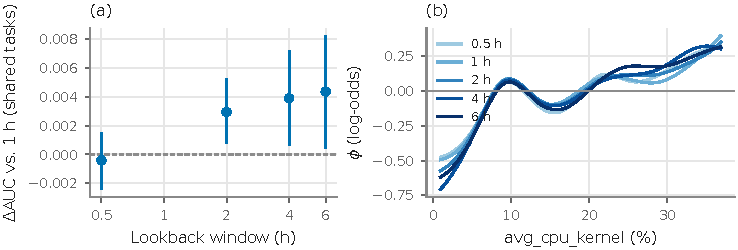
\includegraphics[width=0.85\linewidth]{figures/lookback.pdf}
\caption{Lookback ablation on the original sample. (a) AUC of each window minus the one-hour model on the test tasks both score, with paired 95\% intervals. (b) The \feat{avg_cpu_kernel} curve at each window.}
\label{fig:lookback}
\end{figure}


\section{Discussion}
\label{sec:discussion}

\paragraph{A random split rewards memorisation.} Under the random protocol at most \V{full.random.maxnew} of the \V{full.split.random.s42.ntest} test tasks of a split come from users without training tasks, and \V{rf.full.dup.random.min} to \V{rf.full.dup.random.max} have an exact feature duplicate in training. The models with interactions lead there: LightGBM is \V{full.random.lgbm.absdiff} AUC above \kaam{} on the full trace, and LightGBM and the EBM with pairwise terms are \V{orig.random.lgbm.absdiff} and \V{orig.random.ebmi.absdiff} above it on the original sample. Under the user-grouped protocol that lead is gone: on the four folds without User~1, LightGBM scores \V{full.gnou.lgbm.auc} and the MLP and \kaam{} \V{full.gnou.mlp.auc} and \V{full.gnou.kaam.auc}, and no model is clearly best. This pattern is consistent with the flexible models' random-split gain being knowledge of particular users and of duplicated requests. It does not show that interactions themselves fail to transfer: LightGBM's grouped fits were cut after a few boosting rounds by early stopping on validation users, and a regularised or interaction-constrained boosting model would be needed to test that.

\paragraph{What transfers and what does not.} Two settings matter for a failure predictor in production. For users already in the training data, the features carry over to a later period only weakly: on the last \V{prot.time.test} of the trace every model scores between \V{full.timeknown.minauc} and \V{full.timeknown.maxauc} on known users, although on the validation period just before it, a burst in which User~1 submits \V{rf.full.time.val.u1} of the tasks, the same models scored between \V{full.time.minvalauc} and \V{full.time.maxvalauc}. The trace changes near its end; the failure rate is \V{full.split.time.t.ratetrain} in the training period, \V{full.split.time.t.rateval} in the validation period and \V{full.split.time.t.ratetest} in the test period. For new users the features carry a weak signal at best: the user-grouped AUCs lie between \V{full.grouped.minauc} and \V{full.grouped.maxauc} on the full trace with wide intervals, and the new users of the time-ordered test period, few in number, are scored between \V{full.timenew.minauc} and \V{full.timenew.maxauc}. A deployment could at most support an operator who reviews the recurring pipelines of known users; it should not be used to judge the first jobs of a new user, and its accuracy on a random split describes neither case. Whether frequent retraining would close the gap to a later period is not tested here.

\paragraph{What the audit contributed.} The finding that drives this paper came from reading the model. The \feat{plan_cpu} curve assigns a large rise to one-core requests; the case audit of the most confident catch puts most of its score on that single term; counting the training tasks behind it shows a request submitted almost entirely by User~1; and once User~1 is removed from the training data, one-core tasks fail about as often as other tasks. The same chain explains the most confident false alarm, a one-core task of another user that inherits User~1's term. Each step uses an exact property of the additive model: the curve is the model's whole treatment of the feature, and the contributions are exact SHAP values. Any additive model, the additive EBM included, supports the same chain; the KAN form adds smooth curves with an explicit smoothness penalty, not a different kind of explanation. A global importance score would show that \feat{plan_cpu} matters; it would not show by itself that its effect comes from one user's recurring job.

\paragraph{The smoothness penalty is chosen by the protocol.} On random splits validation preferred no penalty, and the request curves oscillate between observed values; when the validation tasks came from other users or a later period, validation preferred the strongest penalty. A smooth curve is easier to read, and validation prefers it when the validation population differs from the training population.

\paragraph{What changed from the first version.} The first version reported that \kaam{} matched a parameter-matched MLP on one random split of the original sample (\V{v1.kaam.auc} against \V{v1.mlp.auc}) and that every model fell below chance on one user-grouped partition (\kaam{} \V{v1.grouped.kaam}). With five splits, a stronger baseline set and the leak removed, \kaam{} still beats the parameter-matched MLP on the original sample (\V{orig.random.mlp.diff} AUC) but not on the full trace (\V{full.random.mlp.diff}), and it trails LightGBM on both datasets and the EBM with interactions on the original sample. With five user-grouped folds the picture on new users is no longer uniform, and no model is clearly best: the fold AUCs range from \V{full.fold.minauc} to \V{full.fold.maxauc}, and \V{full.fold.nbelow} of the \V{full.fold.npairs} fold-model pairs fall below chance. The first version's single partition was one draw from this spread. The conclusion that the features transfer poorly to new users stands, and it now rests on five folds, two datasets and six models.

\section{Limitations}
\label{sec:limitations}

\paragraph{One trace.} Every result comes from one platform over \V{data.span.days} days, without calendar dates, and the telemetry covers only part of that span. The time-ordered protocol has a single split, so its intervals reflect the resampling of one test period and not the variation between periods.

\paragraph{Neighbour telemetry.} The five machine features describe other jobs on the same machine in the hour before the task started, because the task's own telemetry is recorded almost only when it succeeds. This keeps the features leak-free, but they are a proxy for the conditions the task met.

\paragraph{A selected population.} Requiring recent neighbour telemetry and no missing values keeps \V{data.full.share} of the labelled tasks and raises the failure rate from \V{data.lab.rate} to \V{data.full.rate}. CPU-only tasks and machines with sparse telemetry are under-represented. The results apply to tasks that pass these filters.

\paragraph{The label.} The label follows the trace's status field. The trace does not say whether a \texttt{Terminated} task finished normally or was stopped by its user or the scheduler, and we treat every such task as a non-failure.

\paragraph{First instance only.} For tasks with several instances, only the machine of the first one is described.

\paragraph{Ten features.} The features describe the shape of a request and the recent state of a machine. They contain nothing about the user's code, data or configuration, which earlier studies identify as common causes of failure~\cite{jeon2019philly,zhang2020dlfailures}.

\paragraph{No interactions in \kaam{}.} \kaam{} cannot represent an effect that depends on two features at once. This is the price of reading every feature alone; the gap to LightGBM and to the EBM with pairwise terms measures it on this data.

\paragraph{Correlated features.} The GPU count of a machine and its telemetry move together, so the credit an additive model gives to each of them is not unique; different models can split it differently and all be consistent with the data.

\paragraph{Compute.} All experiments ran on one laptop with \V{data.cpus} logical CPUs. The validation grids are small, the EBMs use package defaults, and on the full trace the EBMs were fitted only on the canonical split; the EBM comparisons under every protocol therefore come from the original sample. The EBM with interactions has one seed outside the random splits of the original sample.

\paragraph{Lookback ablation.} The window comparison uses the original sample, one model and one seed.

\section{Conclusion}
\label{sec:conclusion}

On the full Alibaba PAI 2020 trace, the models with interactions lead on random task-level splits, where many test tasks duplicate a training task. With users held out no model is clearly best, and every model loses much of its random-split accuracy on new users and in the final week of the trace. The readable model located one shortcut behind the random-split scores, a one-core rule learned from one user's recurring job, through its curves, its exact contributions and the training data behind them. Failure predictors for shared clusters should be evaluated with grouped and time-ordered protocols that report known and new users separately and check for duplicated tasks, and a readable model is a practical tool for finding the shortcuts that a random split rewards.

\section*{Acknowledgment}

This paper and its software were prepared with help from Anthropic's Claude and Claude Code, which I used to write much of the implementation code and to draft and revise the text and tables. Every line of generated code and every figure was inspected and verified by me, and responsibility for the accuracy of the findings rests with me alone.


\bibliographystyle{plainnat}
\bibliography{references}

\appendix
\section{Deviations from the protocol}
\label{app:deviations}

The protocol file was written after the datasets were built and before any model was trained on them. Four changes were made afterwards. All four were made before the first read of a test label, and each was recorded in the protocol file with its time and reason; the protocol hash stored with every test access is the hash of the file with all four entries.

\begin{enumerate}
\item \textbf{Early stopping on validation ROC-AUC.} The protocol specified early stopping on validation log loss. Under the time-ordered split the validation failure rate is \V{full.split.time.t.rateval} against \V{full.split.time.t.ratetrain} in training, so an almost untrained network, which predicts about one half for every task, had a lower validation log loss than a trained one. On the original sample all five MLP seeds of the time-ordered split stopped after the first epoch, and one \kaam{} seed did the same; on the full random split two of five MLP seeds reached the former cap of \V{model.oldmaxepochs} epochs. Early stopping for \kaam{}, the MLP and LightGBM now monitors validation ROC-AUC, the selection metric, and the epoch cap of the networks is \V{model.maxepochs}. Every fit made under the old rule was set aside and refitted.
\item \textbf{One seed for both EBMs on the full trace.} With four runner processes sharing two physical cores, one additive EBM fit on a full training split took more than twenty minutes, and five seeds on the thirteen full-trace splits would have added about twenty hours. Both EBMs use seed~0 on the full trace; the original sample measures their seed variation.
\item \textbf{One seed for the EBM with interactions outside the random splits of the original sample.} For the same reason, the EBM with interactions uses five seeds on the five random splits of the original sample and seed~0 under its other protocols. The time-ordered split of the original sample had already started its five seeds and keeps them.
\item \textbf{No EBMs under the protocols on the full trace.} Even with one seed, an additive EBM fit with the package defaults on a full training split (about \V{full.split.random.s42.ntrain} tasks) used more than two hours of CPU time without finishing, so the planned full-trace EBM fits would have taken about sixty hours. On the full trace only the additive EBM of the canonical split is fitted, for the comparison of shape functions; the EBM comparisons under every protocol use the original sample, where both EBMs were fitted on every split.
\end{enumerate}

\section{Phase log}
\label{app:phases}

Table~\ref{tab:phases} lists the phases of the project. Phases one to seven are those of the first version; each was frozen before the next began. The present study adds phases eight to twelve.

\begin{table}[ht]
\centering
\small
\caption{Phases of the project. The first seven phases produced the first version; the last five produced this one.}
\label{tab:phases}
\begin{tabular}{@{}rp{3.6cm}p{8.6cm}@{}}
\toprule
Phase & Data & Content \\
\midrule
1 & synthetic, three features & the architecture recovers known curve shapes \\
2 & \V{v1.dev.tasks} tasks & first training on the trace; the worker-keyed join is found to leak \\
3 & \V{v1.dev.tasks} tasks & smoothness penalty, early stopping and decision threshold \\
4 & \V{v1.dev.tasks} tasks & logistic regression and MLP baselines, SHAP agreement \\
5 & \V{data.orig.tasks} tasks & scale-up, seed and split variance, benchmark, published datasets \\
6 & \V{data.lb.0p5.v1rows} to \V{data.lb.6.v1rows} tasks & lookback ablation and four case audits \\
7 & \V{data.orig.tasks} tasks & one user-grouped partition \\
\midrule
8 & every labelled task & leak fix (clipping and scaling fitted per training split); full-trace build of \V{data.full.tasks} tasks in \V{data.build.minutes} minutes; checks against the first version \\
9 & both datasets & protocol file written before any model was trained \\
10 & both datasets & every model fitted on every split; the three deviations \\
11 & both datasets & test labels read through the logged function (\V{access.n} reads); statistics, interpretability, lookback ablation \\
12 & both datasets & tables, figures and every number generated from the result files; claims audit; independent review \\
\bottomrule
\end{tabular}
\end{table}

\section{Hyperparameters}
\label{app:hyper}

Fixed settings: \kaam{} with \V{model.knots} interior knots, cubic splines, SiLU base term, Adam at learning rate \V{model.lr}, minibatches of \V{model.batch}, patience \V{model.patience} epochs, at most \V{model.maxepochs} epochs, minimum AUC improvement \V{model.mindelta}. MLP with ReLU units and the same loop. Logistic regression with an L2 penalty and the L-BFGS solver. LightGBM with learning rate \V{model.lgbm.lr}, bagging and feature fractions of \V{model.lgbm.bag} (bagging every round), at most \V{model.lgbm.rounds} rounds and patience \V{model.lgbm.es} rounds on validation ROC-AUC. EBMs at the defaults of InterpretML \V{ebm.version}. Validation grids: $\lambda\in$\V{model.lambdas}; $C$ over \V{model.lr.ngrid} values from \V{model.lr.cmin} to \V{model.lr.cmax}; MLP hidden layers \V{model.mlp.shapes} crossed with learning rates \V{model.mlp.lrs}; LightGBM leaves \V{model.lgbm.leaves} crossed with minimum leaf sizes \V{model.lgbm.minleaf}. Table~\ref{tab:hyper} gives the settings chosen on each split.

% Generated by scripts/paper_tables.py. Do not edit.
\begin{table}[t]
\centering
\scriptsize
\setlength{\tabcolsep}{3pt}
\TabCaption{tab:hyper}{Settings chosen on the validation split}{One row per split. $\lambda$: \kaam{} smoothness weight; $C$: inverse L2 strength of logistic regression; MLP: hidden layers and learning rate; LightGBM: leaves and minimum leaf size. Mean best epoch over the five seeds in parentheses for \kaam{} and the MLP.}
\begin{tabular}{@{}llllll@{}}
\toprule
Data & Split & $\lambda$ (epoch) & $C$ & MLP (epoch) & LightGBM \\
\midrule
Full & random s42 & 0 (26) & 0.01 & (12), 0.003 (125) & 127, 20 \\
Full & random s43 & 0 (25) & 0.1 & (8,6), 0.01 (48) & 127, 20 \\
Full & random s44 & 0 (20) & 0.03 & (12), 0.003 (117) & 127, 20 \\
Full & random s45 & 0 (25) & 0.1 & (8,6), 0.01 (67) & 127, 20 \\
Full & random s46 & 0 (23) & 0.003 & (8,6), 0.01 (53) & 127, 20 \\
Full & time t & $10^{-2}$ (6) & 0.1 & (8,6), 0.003 (5) & 31, 200 \\
Full & grouped f0 & 0 (11) & 0.001 & (8,6), 0.003 (12) & 127, 200 \\
Full & grouped f1 & $10^{-2}$ (6) & 0.3 & (12), 0.01 (19) & 127, 200 \\
Full & grouped f2 & $10^{-2}$ (2) & 0.001 & (8,6), 0.01 (5) & 127, 200 \\
Full & grouped f3 & $10^{-2}$ (11) & 0.003 & (12), 0.01 (2) & 31, 200 \\
Full & grouped f4 & $10^{-2}$ (15) & 0.003 & (8,6), 0.003 (3) & 31, 200 \\
Full & louo d1 & 0 (21) & 0.003 & (8,6), 0.01 (41) & 127, 20 \\
Full & louo d14 & 0 (41) & 0.001 & (8,6), 0.01 (66) & 127, 20 \\
\midrule
Original & random s42 & $10^{-4}$ (42) & 0.3 & (8,6), 0.003 (108) & 31, 20 \\
Original & random s43 & $10^{-4}$ (41) & 0.03 & (8,6), 0.003 (98) & 31, 20 \\
Original & random s44 & 0 (49) & 0.01 & (8,6), 0.003 (110) & 127, 20 \\
Original & random s45 & $10^{-3}$ (33) & 0.3 & (8,6), 0.003 (103) & 31, 20 \\
Original & random s46 & $10^{-4}$ (39) & 0.03 & (8,6), 0.003 (119) & 31, 20 \\
Original & time t & $10^{-2}$ (4) & 10 & (8,6), 0.003 (20) & 31, 200 \\
Original & grouped f0 & $10^{-2}$ (1) & 30 & (12), 0.003 (1) & 127, 20 \\
Original & grouped f1 & $10^{-4}$ (13) & 0.001 & (12), 0.003 (16) & 127, 20 \\
Original & grouped f2 & $10^{-2}$ (107) & 0.1 & (8,6), 0.01 (14) & 127, 20 \\
Original & grouped f3 & $10^{-2}$ (46) & 30 & (12), 0.003 (88) & 127, 200 \\
Original & grouped f4 & $10^{-2}$ (18) & 0.03 & (12), 0.003 (29) & 127, 20 \\
Original & louo d1 & $10^{-4}$ (51) & 0.01 & (12), 0.01 (59) & 31, 20 \\
Original & louo d14 & $10^{-3}$ (62) & 0.03 & (12), 0.01 (31) & 127, 20 \\
\bottomrule
\end{tabular}
\TabNotes
\end{table}


\section{Test-access log}
\label{app:access}

Test labels can be obtained only through one function, which appends a line to \path{results/test_access_log.jsonl} for every call. The log holds \V{access.n} reads between \V{access.first} and \V{access.last}, all after the last model was fitted, and all with the protocol hash \V{access.sha}. Table~\ref{tab:access} groups them.

% Generated by scripts/paper_tables.py. Do not edit.
\begin{table*}[t]
\centering
\scriptsize
\setlength{\tabcolsep}{3pt}
\TabCaption{tab:access}{Test-access log}{Every read of test labels, grouped by dataset, protocol and purpose (time of the first read in each group, UTC). Each entry of \texttt{results/test\_access\_log.jsonl} records the SHA-256 of the protocol file at that moment; all entries carry the same hash.}
\begin{tabular}{@{}llllrp{5.4cm}@{}}
\toprule
First read (UTC) & Data & Protocol & Splits & Test tasks & Purpose \\
\midrule
2026-11-23 16:20:23 & original & random & s42, s43, s44, s45, s46 & 14,170 & score saved test predictions \texttt{analyze.py} \\
2026-11-23 16:20:23 & original & time & t & 2,834 & score saved test predictions \texttt{analyze.py} \\
2026-11-23 16:20:23 & original & grouped & f0, f1, f2, f3, f4 & 18,890 & score saved test predictions \texttt{analyze.py} \\
2026-11-23 16:20:23 & original & louo & d1, d14 & 3,809 & score saved test predictions \texttt{analyze.py} \\
2026-11-23 16:20:24 & full & random & s42, s43, s44, s45, s46 & 404,865 & score saved test predictions \texttt{analyze.py} \\
2026-11-23 16:20:24 & full & time & t & 80,973 & score saved test predictions \texttt{analyze.py} \\
2026-11-23 16:20:24 & full & grouped & f0, f1, f2, f3, f4 & 539,816 & score saved test predictions \texttt{analyze.py} \\
2026-11-23 16:20:24 & full & louo & d1, d14 & 108,874 & score saved test predictions \texttt{analyze.py} \\
2026-11-23 16:20:55 & lookback-1h & lookback & 1h & 2,834 & lookback ablation \texttt{lookback\_v2.py} \\
2026-11-23 16:20:55 & lookback-0.5h & lookback & 0.5h & 2,671 & lookback ablation \texttt{lookback\_v2.py} \\
2026-11-23 16:20:56 & lookback-2h & lookback & 2h & 2,930 & lookback ablation \texttt{lookback\_v2.py} \\
2026-11-23 16:20:58 & lookback-4h & lookback & 4h & 2,988 & lookback ablation \texttt{lookback\_v2.py} \\
2026-11-23 16:21:00 & lookback-6h & lookback & 6h & 3,011 & lookback ablation \texttt{lookback\_v2.py} \\
2026-11-23 16:21:49 & full & random & s42 & 80,973 & case audits on the canonical KAAM \texttt{interpret\_v2.py} \\
2026-11-23 20:37:37 & full & review & all & 0 & independent review: the reviewer read labels directly from data/processed/v2/full\_1h.parquet for spot checks, outside kanvas/testaccess.py; no model, setting or protocol was changed as a result  \\
2026-11-23 20:39:02 & full & grouped & f0, f1, f2, f3, f4 & 539,816 & post hoc review analysis \texttt{posthoc\_review.py} \\
2026-11-23 21:02:50 & full & random & s42, s43, s44, s45, s46 & 404,865 & post hoc review analysis \texttt{posthoc\_review.py} \\
2026-11-23 21:05:05 & full & louo & d1, d14 & 108,874 & post hoc review analysis \texttt{posthoc\_review.py} \\
\bottomrule
\end{tabular}
\TabNotes
\end{table*}


\section{Further results}
\label{app:more}

Table~\ref{tab:comp_full} lists every paired comparison on the full trace, and Tables~\ref{tab:comp_orig}, \ref{tab:calib_orig} and~\ref{tab:grouped_orig} repeat the comparisons, the calibration metrics and the per-fold results on the original sample.

% Generated by scripts/paper_tables.py. Do not edit.
\begin{table}[t]
\centering
\small
\setlength{\tabcolsep}{4pt}
\TabCaption{tab:comp_full}{Paired comparisons of \kaam{} with every other model, full trace}{$\Delta$AUC is \kaam{} minus the other model; positive values favour \kaam{}. Paired bootstrap over the test sets of the protocol; $p$-values Holm-adjusted within each protocol (three comparisons on the full trace, five on the original sample). n.s.: not significant.}
\begin{tabular}{@{}llrcr@{}}
\toprule
Protocol & \kaam{} minus & $\Delta$AUC & 95\% CI & $p_{\mathrm{Holm}}$ \\
\midrule
Random & Logistic regression & +0.033 & [0.032, 0.035] & 0.003 \\
 & MLP & $-$0.038 & [$-$0.040, $-$0.037] & 0.003 \\
 & LightGBM & $-$0.134 & [$-$0.136, $-$0.133] & 0.003 \\
\addlinespace
Time, all & Logistic regression & +0.018 & [0.016, 0.021] & 0.003 \\
 & MLP & $-$0.002 & [$-$0.005, 0.001] & 0.162 (n.s.) \\
 & LightGBM & $-$0.005 & [$-$0.012, 0.001] & 0.162 (n.s.) \\
\addlinespace
Time, known users & Logistic regression & +0.017 & [0.014, 0.020] & 0.003 \\
 & MLP & $-$0.002 & [$-$0.005, 0.001] & 0.242 (n.s.) \\
 & LightGBM & $-$0.003 & [$-$0.009, 0.003] & 0.417 (n.s.) \\
\addlinespace
Time, new users & Logistic regression & +0.004 & [$-$0.025, 0.033] & 0.768 (n.s.) \\
 & MLP & $-$0.016 & [$-$0.041, 0.009] & 0.420 (n.s.) \\
 & LightGBM & $-$0.068 & [$-$0.106, $-$0.027] & 0.009 \\
\addlinespace
User-grouped & Logistic regression & +0.041 & [0.011, 0.067] & 0.021 \\
 & MLP & +0.004 & [$-$0.032, 0.023] & 0.933 (n.s.) \\
 & LightGBM & +0.076 & [$-$0.031, 0.107] & 0.562 (n.s.) \\
\addlinespace
Without User~1 & Logistic regression & +0.047 & [0.042, 0.053] & 0.003 \\
 & MLP & $-$0.018 & [$-$0.022, $-$0.014] & 0.003 \\
 & LightGBM & $-$0.141 & [$-$0.147, $-$0.136] & 0.003 \\
\addlinespace
Without Users~1, 4 & Logistic regression & +0.042 & [0.037, 0.047] & 0.003 \\
 & MLP & $-$0.026 & [$-$0.031, $-$0.021] & 0.003 \\
 & LightGBM & $-$0.133 & [$-$0.139, $-$0.127] & 0.003 \\
\bottomrule
\end{tabular}
\TabNotes
\end{table}

% Generated by scripts/paper_tables.py. Do not edit.
\begin{table}[t]
\centering
\small
\setlength{\tabcolsep}{4pt}
\TabCaption{tab:comp_orig}{Paired comparisons of \kaam{} with every other model, original sample}{Same layout as Table~\ref{tab:comp_full}.}
\begin{tabular}{@{}llrcr@{}}
\toprule
Protocol & \kaam{} minus & $\Delta$AUC & 95\% CI & $p_{\mathrm{Holm}}$ \\
\midrule
Random & Logistic regression & +0.022 & [0.015, 0.029] & 0.005 \\
 & MLP & +0.022 & [0.016, 0.028] & 0.005 \\
 & LightGBM & $-$0.066 & [$-$0.073, $-$0.058] & 0.005 \\
 & EBM, additive & $-$0.011 & [$-$0.014, $-$0.008] & 0.005 \\
 & EBM, pairwise & $-$0.058 & [$-$0.066, $-$0.051] & 0.005 \\
\addlinespace
Time, all & Logistic regression & +0.007 & [$-$0.017, 0.031] & 1.000 (n.s.) \\
 & MLP & +0.071 & [0.044, 0.099] & 0.005 \\
 & LightGBM & $-$0.024 & [$-$0.047, $-$0.001] & 0.164 (n.s.) \\
 & EBM, additive & 0.000 & [$-$0.023, 0.023] & 1.000 (n.s.) \\
 & EBM, pairwise & +0.022 & [$-$0.014, 0.057] & 0.639 (n.s.) \\
\addlinespace
Time, known users & Logistic regression & +0.013 & [$-$0.011, 0.039] & 0.576 (n.s.) \\
 & MLP & +0.070 & [0.042, 0.100] & 0.005 \\
 & LightGBM & $-$0.018 & [$-$0.043, 0.007] & 0.513 (n.s.) \\
 & EBM, additive & +0.007 & [$-$0.018, 0.033] & 0.609 (n.s.) \\
 & EBM, pairwise & +0.038 & [0.000, 0.077] & 0.204 (n.s.) \\
\addlinespace
Time, new users & Logistic regression & $-$0.049 & [$-$0.162, 0.057] & 1.000 (n.s.) \\
 & MLP & $-$0.032 & [$-$0.154, 0.090] & 1.000 (n.s.) \\
 & LightGBM & $-$0.036 & [$-$0.147, 0.070] & 1.000 (n.s.) \\
 & EBM, additive & $-$0.017 & [$-$0.112, 0.077] & 1.000 (n.s.) \\
 & EBM, pairwise & $-$0.023 & [$-$0.127, 0.082] & 1.000 (n.s.) \\
\addlinespace
User-grouped & Logistic regression & +0.059 & [0.004, 0.098] & 0.136 (n.s.) \\
 & MLP & +0.080 & [0.042, 0.096] & 0.005 \\
 & LightGBM & +0.118 & [$-$0.004, 0.148] & 0.231 (n.s.) \\
 & EBM, additive & +0.130 & [$-$0.014, 0.160] & 0.312 (n.s.) \\
 & EBM, pairwise & +0.116 & [$-$0.025, 0.150] & 0.312 (n.s.) \\
\addlinespace
Without User~1 & Logistic regression & +0.036 & [0.012, 0.060] & 0.006 \\
 & MLP & +0.017 & [$-$0.003, 0.037] & 0.095 (n.s.) \\
 & LightGBM & $-$0.058 & [$-$0.082, $-$0.034] & 0.005 \\
 & EBM, additive & $-$0.023 & [$-$0.039, $-$0.008] & 0.010 \\
 & EBM, pairwise & $-$0.054 & [$-$0.077, $-$0.030] & 0.005 \\
\addlinespace
Without Users~1, 4 & Logistic regression & +0.026 & [0.004, 0.046] & 0.034 \\
 & MLP & +0.097 & [0.067, 0.126] & 0.005 \\
 & LightGBM & $-$0.046 & [$-$0.078, $-$0.012] & 0.018 \\
 & EBM, additive & $-$0.019 & [$-$0.036, $-$0.003] & 0.034 \\
 & EBM, pairwise & $-$0.058 & [$-$0.088, $-$0.028] & 0.005 \\
\bottomrule
\end{tabular}
\TabNotes
\end{table}

% Generated by scripts/paper_tables.py. Do not edit.
\begin{table}[t]
\centering
\small
\setlength{\tabcolsep}{3pt}
\TabCaption{tab:calib_orig}{Precision-recall and calibration, original sample}{Same layout as Table~\ref{tab:calib_full}.}
\begin{tabular}{@{}lccccccccc@{}}
\toprule
 & \multicolumn{3}{c}{Random} & \multicolumn{3}{c}{Time, all} & \multicolumn{3}{c}{User-grouped} \\
\cmidrule(lr){2-4}\cmidrule(lr){5-7}\cmidrule(lr){8-10}
Model & PR-AUC & Brier & ECE & PR-AUC & Brier & ECE & PR-AUC & Brier & ECE \\
\midrule
KAAM & 0.623 & 0.155 & 0.049 & 0.220 & 0.142 & 0.044 & 0.337 & 0.176 & 0.122 \\
Logistic regression & 0.530 & 0.172 & 0.096 & 0.203 & 0.145 & 0.054 & 0.314 & 0.185 & 0.136 \\
MLP & 0.561 & 0.181 & 0.098 & 0.192 & 0.180 & 0.136 & 0.293 & 0.221 & 0.199 \\
LightGBM & 0.706 & 0.134 & 0.027 & 0.222 & 0.142 & 0.045 & 0.247 & 0.206 & 0.142 \\
EBM, additive & 0.625 & 0.152 & 0.030 & 0.193 & 0.148 & 0.047 & 0.241 & 0.210 & 0.141 \\
EBM, pairwise & 0.695 & 0.137 & 0.024 & 0.200 & 0.153 & 0.068 & 0.257 & 0.208 & 0.151 \\
\bottomrule
\end{tabular}
\TabNotes
\end{table}

% Generated by scripts/paper_tables.py. Do not edit.
\begin{table*}[t]
\centering
\footnotesize
\setlength{\tabcolsep}{3pt}
\TabCaption{tab:grouped_orig}{User-grouped folds on the original sample}{Same layout as Table~\ref{tab:grouped_full}.}
\begin{tabular}{@{}lcccccccc@{}}
\toprule
Model & Fold 0 & Fold 1 & Fold 2 & Fold 3 & Fold 4 & Mean & 95\% CI & $p_{\mathrm{Holm}}$ vs.\ 0.5 \\
\midrule
KAAM & 0.505 & 0.531 & 0.728 & 0.624 & 0.710 & 0.620 & [0.551, 0.641] & 0.006 \\
Logistic regression & 0.593 & 0.455 & 0.551 & 0.459 & 0.745 & 0.561 & [0.487, 0.601] & 0.765 \\
MLP & 0.478 & 0.464 & 0.494 & 0.569 & 0.693 & 0.540 & [0.486, 0.564] & 1.000 \\
LightGBM & 0.572 & 0.509 & 0.432 & 0.613 & 0.383 & 0.502 & [0.469, 0.577] & 1.000 \\
EBM, additive & 0.559 & 0.530 & 0.330 & 0.618 & 0.409 & 0.489 & [0.454, 0.588] & 1.000 \\
EBM, pairwise & 0.550 & 0.528 & 0.428 & 0.643 & 0.369 & 0.504 & [0.466, 0.599] & 1.000 \\
\midrule
Test users & 171 & 196 & 3 & 200 & 168 &  &  &  \\
Test tasks & 3,039 & 3,035 & 6,693 & 3,037 & 3,086 &  &  &  \\
One-core failure rate, train & 77.2\% & 80.3\% & 18.6\% & 76.7\% & 83.7\% &  &  &  \\
Other failure rate, train & 20.5\% & 20.7\% & 19.7\% & 20.8\% & 19.3\% &  &  &  \\
One-core failure rate, test & 46.3\% & 20.5\% & 87.5\% & 47.1\% & 6.7\% &  &  &  \\
Other failure rate, test & 18.1\% & 18.6\% & 20.6\% & 18.2\% & 22.6\% &  &  &  \\
AUC of $-$\feat{plan_cpu}, train & 0.722 & 0.721 & 0.533 & 0.722 & 0.693 &  &  &  \\
AUC of $-$\feat{plan_cpu}, test & 0.471 & 0.417 & 0.777 & 0.426 & 0.721 &  &  &  \\
\bottomrule
\end{tabular}
\TabNotes
\end{table*}



\end{document}
